         \chapter{Electric circuits}
    \setcounter{figure}{1}
    \setcounter{subfigure}{1}
    \label{f13bac5321b85aca0e213ebdf4f72465}
    
    
    
    
       
         \section{ Introduction and key concepts}
    \nopagebreak
            \label{m38771} $ \hspace{-5pt}\begin{array}{cccccccccccc}   
\includegraphics[width=0.75cm]{col11305.imgs/summary_fullmarks.png} &   
\includegraphics[width=0.75cm]{col11305.imgs/summary_simulation.png} &   \end{array} $ \hspace{2 pt}\raisebox{-5 pt}{} {(section shortcode: P10074 )} \par 
    
    
    
    
    
    
  
    \label{m38771*cid2}
            \subsection{ Electric Circuits}
            \nopagebreak
            
      
      \label{m38771*id62184}People all over the world depend on electricity to provide power for most appliances in the home and at work. For example, fluorescent lights, electric heating and cooking (on electric stoves), all depend on electricity to work.
To realise just how big an impact electricity has on our daily lives, just think about what happens when there is a power
failure or load shedding.\par 
\label{m38771*secfhsst!!!underscore!!!id72}
            \subsubsection{  Discussion : Uses of electricity }
            \nopagebreak
            
      \label{m38771*id62198}With a partner, take the following topics and, for each topic, write down at least 5 items/appliances/machines which need
electricity to work. Try not to use the same item more than once.\par 
      \label{m38771*id62544}\begin{itemize}[noitemsep]
            \label{m38771*uid1}\item At home
\label{m38771*uid2}\item At school
\label{m38771*uid3}\item At the hospital
\label{m38771*uid4}\item In the city
\end{itemize}
        
      \label{m38771*id62592}Once you have finished making your lists, compare with the lists of other people in your class. (Save your lists somewhere safe for later because there will be another activity for which you'll need them.)\par 
      \label{m38771*id62597}When you start comparing, you should notice that there are many different items which we use in our daily lives which rely on electricity to work!
 \par 

\label{m38771*notfhsst!!!underscore!!!id89}
\begin{tabular}{cc}
	   \hspace*{-50pt}\raisebox{-8 mm}{ 
\includegraphics[width=0.5in]{col11305.imgs/pstip2.png}  }& 

	\begin{minipage}{0.85\textwidth}
	\begin{note}
      {tip: }\textbf{Safety Warning:}
We believe in experimenting and learning about physics at every opportunity, BUT
playing with electricity and electrical appliances can be \textbf{EXTREMELY DANGEROUS}! Do not try to build
homemade circuits alone. Make sure you have someone with you who knows if what you are doing is safe.
Normal electrical outlets are dangerous. Treat electricity with respect in your everyday life. Do not touch exposed wires and do not approach downed power lines.
	\end{note}
	\end{minipage}
	\end{tabular}
	\par
      
      \label{m38771*uid5}
            \subsubsection{ Closed circuits}
            \nopagebreak
            
        
        \label{m38771*id62637}In the following activity we will investigate what is needed to cause charge to flow in an electric circuit.\par 
\label{m38771*secfhsst!!!underscore!!!id97}
            \subsubsection{ Experiment : Closed circuits }
            \nopagebreak
            \label{m38771*id62648}\noindent{}\textbf{Aim:}
          
To determine what is required to make electrical charges flow.
In this experiment, we will use a lightbulb to check whether electrical charge is flowing in the circuit or not. If charge is flowing, the lightbulb should glow. On the other hand, if no charge is flowing, the lightbulb will not glow.\par 
        \label{m38771*id62665}\noindent{}\textbf{Apparatus:}
          
        You will need a small lightbulb which is attached to a metal conductor (e.g. a bulb from a school electrical kit), some connecting wires and a battery.\par 
        \label{m38771*id62679}\noindent{}\textbf{Method:}
          
        Take the apparatus items and try to connect them in a way that you cause the light bulb to glow (i.e. charge flows in the circuit).\par 
        \label{m38771*id62694}\noindent{}\textbf{Questions:}
          
        \label{m38771*id62702}\begin{enumerate}[noitemsep, label=\textbf{\arabic*}. ] 
            \label{m38771*uid6}\item Once you have arranged your circuit elements to make the lightbulb glow, draw your circuit.
\label{m38771*uid7}\item What can you say about how the battery is connected? (i.e. does it have one or two connecting leads attached? Where are they attached?)
\label{m38771*uid8}\item What can you say about how the light bulb is connected in your circuit? (i.e. does it connect to one or two connecting leads, and where are they attached?)
\label{m38771*uid9}\item Are there any items in your circuit which are not attached to something? In other words, are there any gaps in your circuit?
\end{enumerate}
        \par 
        \label{m38771*id62757}Write down your conclusion about what is needed to make an electric circuit work and charge to flow.
 \par 

        \label{m38771*id62768}In the experiment above, you will have seen that the light bulb only glows when there is a \textsl{closed} circuit i.e. there are no gaps in the circuit and all the circuit elements are connected in a \textsl{closed loop}. Therefore, in order for charges to flow, a closed circuit and an energy source (in this case the battery) are needed. (Note: you do not have to have a lightbulb in the circuit! We used this as a check that charge was flowing.)\par 
\label{m38771*fhsst!!!underscore!!!id128}\begin{definition}
	  \begin{tabular*}{15 cm}{m{15 mm}m{}}
	\hspace*{-50pt}  
\includegraphics[width=0.5in]{col11305.imgs/psflag2.png}   & \Definition{   \label{id2477990}\textbf{ Electric circuit }} { \label{m38771*meaningfhsst!!!underscore!!!id128}
        \label{m38771*id62792}An electric circuit is a closed path (with no breaks or gaps) along which electrical charges (electrons) flow powered by an energy source. \par 
         } 
      \end{tabular*}
      \end{definition}

      
      \label{m38771*uid10}
            \subsubsection{ Representing electric circuits}
            \nopagebreak
            
        
        \label{m38771*uid11}
            \subsubsection{ Components of electrical circuits}
            \nopagebreak
            
          
          \label{m38771*id62821}Some common elements (components) which can be found in electrical circuits include light bulbs, batteries, connecting leads, switches, resistors, voltmeters and ammeters. You will learn more about these items in later sections, but it is important to know what their symbols are and how to represent them in circuit diagrams. Below is a table with the items and their symbols:\par 
          
    % \textbf{m38516*uid12}\par
    
    % how many colspecs?  3
          % name: cnx:colspec
            % colnum: 1
            % colwidth: 10*
            % latex-name: columna
            % colname: 
            % align/tgroup-align/default: //left
            % -------------------------
            % name: cnx:colspec
            % colnum: 2
            % colwidth: 10*
            % latex-name: columnb
            % colname: 
            % align/tgroup-align/default: //left
            % -------------------------
            % name: cnx:colspec
            % colnum: 3
            % colwidth: 10*
            % latex-name: columnc
            % colname: 
            % align/tgroup-align/default: //left
            % -------------------------
      
    
    \setlength\mytablespace{6\tabcolsep}
    \addtolength\mytablespace{4\arrayrulewidth}
    \setlength\mytablewidth{\linewidth}
        
    
    \setlength\mytableroom{\mytablewidth}
    \addtolength\mytableroom{-\mytablespace}
    
    \setlength\myfixedwidth{0pt}
    \setlength\mystarwidth{\mytableroom}
        \addtolength\mystarwidth{-\myfixedwidth}
        \divide\mystarwidth 30
        
    
            % ----- Table with code
            
    % \begin{table}[H]
    % \\ '' '0'
    
        \begin{center}
      
      \label{m38516*uid12}
      
    \noindent
    \tabletail{%
        \hline
        \multicolumn{3}{|p{\mytableroom}|}{\raggedleft \small \sl continued on next page}\\
        \hline
      }
      \tablelasttail{}
      \begin{xtabular*}{\mytablewidth}[t]{|p{10\mystarwidth}|p{10\mystarwidth}|p{10\mystarwidth}|}\hline
    % count in rowspan-info-nodeset: 3
    % align/colidx: left,1
    
    % rowcount: '0' | start: 'false' | colidx: '1'
    
        % Formatting a regular cell and recurring on the next sibling
        
                    \textbf{Component}
                   &
      % align/colidx: left,2
    
    % rowcount: '0' | start: 'false' | colidx: '2'
    
        % Formatting a regular cell and recurring on the next sibling
        
                    \textbf{Symbol}
                   &
      % align/colidx: left,3
    
    % rowcount: '0' | start: 'false' | colidx: '3'
    
        % Formatting a regular cell and recurring on the next sibling
        
                    \textbf{Usage}
                  % make-rowspan-placeholders
    % rowspan info: col1 '0' | 'false' | '' || col2 '0' | 'false' | '' || col3 '0' | 'false' | ''
     \tabularnewline\cline{1-1}\cline{2-2}\cline{3-3}
      %--------------------------------------------------------------------
    % align/colidx: left,1
    
    % rowcount: '0' | start: 'false' | colidx: '1'
    
        % Formatting a regular cell and recurring on the next sibling
        light bulb &
      % align/colidx: left,2
    
    % rowcount: '0' | start: 'false' | colidx: '2'
    
        % Formatting a regular cell and recurring on the next sibling
        
                    
    \setcounter{subfigure}{0}

\label{m38516*id62893}
    \begin{center}
    \label{m38516*id62893!!!underscore!!!media}\label{m38516*id62893!!!underscore!!!printimage}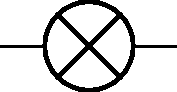
\includegraphics[width=0.2\textwidth]{col11305.imgs/m38516_PG10C9_001.png} % m38516;PG10C9\_001.png;;;6.0;8.5;
        
      \vspace{2pt}
    \vspace{.1in}
    
    \end{center}



    \addtocounter{footnote}{-0}
    
                   &
      % align/colidx: left,3
    
    % rowcount: '0' | start: 'false' | colidx: '3'
    
        % Formatting a regular cell and recurring on the next sibling
        glows when charge moves through it% make-rowspan-placeholders
    % rowspan info: col1 '0' | 'false' | '' || col2 '0' | 'false' | '' || col3 '0' | 'false' | ''
     \tabularnewline\cline{1-1}\cline{2-2}\cline{3-3}
      %--------------------------------------------------------------------
    % align/colidx: left,1
    
    % rowcount: '0' | start: 'false' | colidx: '1'
    
        % Formatting a regular cell and recurring on the next sibling
        battery &
      % align/colidx: left,2
    
    % rowcount: '0' | start: 'false' | colidx: '2'
    
        % Formatting a regular cell and recurring on the next sibling
        
                    
    \setcounter{subfigure}{0}

\label{m38516*id62930}
    \begin{center}
    \label{m38516*id62930!!!underscore!!!media}\label{m38516*id62930!!!underscore!!!printimage}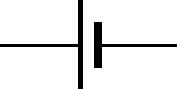
\includegraphics[width=0.2\textwidth]{col11305.imgs/m38516_PG10C9_002.png} % m38516;PG10C9\_002.png;;;6.0;8.5;
        
      \vspace{2pt}
    \vspace{\rubberspace}\par \begin{cnxcaption}
	  \small \textbf{Figure 23.2: }The longer line shows the positive (+) side of the battery, the shorter line shows the (-) side of the battery.
	\end{cnxcaption}
      
    \vspace{.1in}
    
    \end{center}



    \addtocounter{footnote}{-0}
    
                   &
      % align/colidx: left,3
    
    % rowcount: '0' | start: 'false' | colidx: '3'
    
        % Formatting a regular cell and recurring on the next sibling
        provides energy for charge to move - conventional current flow from positive to negative through a circuit% make-rowspan-placeholders
    % rowspan info: col1 '0' | 'false' | '' || col2 '0' | 'false' | '' || col3 '0' | 'false' | ''
     \tabularnewline\cline{1-1}\cline{2-2}\cline{3-3}
      %--------------------------------------------------------------------
    % align/colidx: left,1
    
    % rowcount: '0' | start: 'false' | colidx: '1'
    
        % Formatting a regular cell and recurring on the next sibling
        switch &
      % align/colidx: left,2
    
    % rowcount: '0' | start: 'false' | colidx: '2'
    
        % Formatting a regular cell and recurring on the next sibling
        
                    
    \setcounter{subfigure}{0}

\label{m38516*id62966}
    \begin{center}
    \label{m38516*id62966!!!underscore!!!media}\label{m38516*id62966!!!underscore!!!printimage}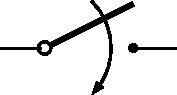
\includegraphics[width=0.2\textwidth]{col11305.imgs/m38516_PG10C9_003.png} % m38516;PG10C9\_003.png;;;6.0;8.5;
        
      \vspace{2pt}
    \vspace{.1in}
    
    \end{center}



    \addtocounter{footnote}{-0}
    
                   &
      % align/colidx: left,3
    
    % rowcount: '0' | start: 'false' | colidx: '3'
    
        % Formatting a regular cell and recurring on the next sibling
        allows a circuit to be open or closed% make-rowspan-placeholders
    % rowspan info: col1 '0' | 'false' | '' || col2 '0' | 'false' | '' || col3 '0' | 'false' | ''
     \tabularnewline\cline{1-1}\cline{2-2}\cline{3-3}
      %--------------------------------------------------------------------
    % align/colidx: left,1
    
    % rowcount: '0' | start: 'false' | colidx: '1'
    
        % Formatting a regular cell and recurring on the next sibling
        resistor &
      % align/colidx: left,2
    
    % rowcount: '0' | start: 'false' | colidx: '2'
    
        % Formatting a regular cell and recurring on the next sibling
        
                    
    \setcounter{subfigure}{0}

\label{m38516*id63001}
    \begin{center}
    \label{m38516*id63001!!!underscore!!!media}\label{m38516*id63001!!!underscore!!!printimage}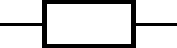
\includegraphics[width=0.2\textwidth]{col11305.imgs/m38516_PG10C9_004.png} % m38516;PG10C9\_004.png;;;6.0;8.5;
        
      \vspace{2pt}
    \vspace{.1in}
    
    \end{center}



    \addtocounter{footnote}{-0}
    
                   &
      % align/colidx: left,3
    
    % rowcount: '0' | start: 'false' | colidx: '3'
    
        % Formatting a regular cell and recurring on the next sibling
        resists the flow of charge% make-rowspan-placeholders
    % rowspan info: col1 '0' | 'false' | '' || col2 '0' | 'false' | '' || col3 '0' | 'false' | ''
     \tabularnewline\cline{1-1}\cline{2-2}\cline{3-3}
      %--------------------------------------------------------------------
    % align/colidx: left,1
    
    % rowcount: '0' | start: 'false' | colidx: '1'
    
        % Formatting a regular cell and recurring on the next sibling
         &
      % align/colidx: left,2
    
    % rowcount: '0' | start: 'false' | colidx: '2'
    
        % Formatting a regular cell and recurring on the next sibling
        OR &
      % align/colidx: left,3
    
    % rowcount: '0' | start: 'false' | colidx: '3'
    
        % Formatting a regular cell and recurring on the next sibling
        % make-rowspan-placeholders
    % rowspan info: col1 '0' | 'false' | '' || col2 '0' | 'false' | '' || col3 '0' | 'false' | ''
     \tabularnewline\cline{1-1}\cline{2-2}\cline{3-3}
      %--------------------------------------------------------------------
    % align/colidx: left,1
    
    % rowcount: '0' | start: 'false' | colidx: '1'
    
        % Formatting a regular cell and recurring on the next sibling
         &
      % align/colidx: left,2
    
    % rowcount: '0' | start: 'false' | colidx: '2'
    
        % Formatting a regular cell and recurring on the next sibling
        
                    
    \setcounter{subfigure}{0}

\label{m38516*id63056}
    \begin{center}
    \label{m38516*id63056!!!underscore!!!media}\label{m38516*id63056!!!underscore!!!printimage}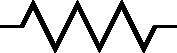
\includegraphics[width=0.2\textwidth]{col11305.imgs/m38516_PG10C9_005.png} % m38516;PG10C9\_005.png;;;6.0;8.5;
        
      \vspace{2pt}
    \vspace{.1in}
    
    \end{center}



    \addtocounter{footnote}{-0}
    
                   &
      % align/colidx: left,3
    
    % rowcount: '0' | start: 'false' | colidx: '3'
    
        % Formatting a regular cell and recurring on the next sibling
        % make-rowspan-placeholders
    % rowspan info: col1 '0' | 'false' | '' || col2 '0' | 'false' | '' || col3 '0' | 'false' | ''
     \tabularnewline\cline{1-1}\cline{2-2}\cline{3-3}
      %--------------------------------------------------------------------
    % align/colidx: left,1
    
    % rowcount: '0' | start: 'false' | colidx: '1'
    
        % Formatting a regular cell and recurring on the next sibling
        voltmeter &
      % align/colidx: left,2
    
    % rowcount: '0' | start: 'false' | colidx: '2'
    
        % Formatting a regular cell and recurring on the next sibling
        
                    
    \setcounter{subfigure}{0}

\label{m38516*id63089}
    \begin{center}
    \label{m38516*id63089!!!underscore!!!media}\label{m38516*id63089!!!underscore!!!printimage}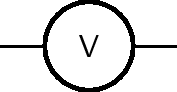
\includegraphics[width=0.2\textwidth]{col11305.imgs/m38516_PG10C9_006.png} % m38516;PG10C9\_006.png;;;6.0;8.5;
        
      \vspace{2pt}
    \vspace{.1in}
    
    \end{center}



    \addtocounter{footnote}{-0}
    
                   &
      % align/colidx: left,3
    
    % rowcount: '0' | start: 'false' | colidx: '3'
    
        % Formatting a regular cell and recurring on the next sibling
        measures potential difference% make-rowspan-placeholders
    % rowspan info: col1 '0' | 'false' | '' || col2 '0' | 'false' | '' || col3 '0' | 'false' | ''
     \tabularnewline\cline{1-1}\cline{2-2}\cline{3-3}
      %--------------------------------------------------------------------
    % align/colidx: left,1
    
    % rowcount: '0' | start: 'false' | colidx: '1'
    
        % Formatting a regular cell and recurring on the next sibling
        ammeter &
      % align/colidx: left,2
    
    % rowcount: '0' | start: 'false' | colidx: '2'
    
        % Formatting a regular cell and recurring on the next sibling
        
                    
    \setcounter{subfigure}{0}

\label{m38516*id63126}
    \begin{center}
    \label{m38516*id63126!!!underscore!!!media}\label{m38516*id63126!!!underscore!!!printimage}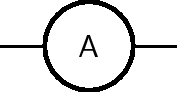
\includegraphics[width=0.2\textwidth]{col11305.imgs/m38516_PG10C9_007.png} % m38516;PG10C9\_007.png;;;6.0;8.5;
        
      \vspace{2pt}
    \vspace{.1in}
    
    \end{center}



    \addtocounter{footnote}{-0}
    
                   &
      % align/colidx: left,3
    
    % rowcount: '0' | start: 'false' | colidx: '3'
    
        % Formatting a regular cell and recurring on the next sibling
        measures current in a circuit% make-rowspan-placeholders
    % rowspan info: col1 '0' | 'false' | '' || col2 '0' | 'false' | '' || col3 '0' | 'false' | ''
     \tabularnewline\cline{1-1}\cline{2-2}\cline{3-3}
      %--------------------------------------------------------------------
    % align/colidx: left,1
    
    % rowcount: '0' | start: 'false' | colidx: '1'
    
        % Formatting a regular cell and recurring on the next sibling
        connecting lead &
      % align/colidx: left,2
    
    % rowcount: '0' | start: 'false' | colidx: '2'
    
        % Formatting a regular cell and recurring on the next sibling
        
                    
    \setcounter{subfigure}{0}

\label{m38516*id63163}
    \begin{center}
    \label{m38516*id63163!!!underscore!!!media}\label{m38516*id63163!!!underscore!!!printimage}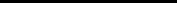
\includegraphics[width=0.2\textwidth]{col11305.imgs/m38516_PG10C9_008.png} % m38516;PG10C9\_008.png;;;6.0;8.5;
        
      \vspace{2pt}
    \vspace{.1in}
    
    \end{center}



    \addtocounter{footnote}{-0}
    
                   &
      % align/colidx: left,3
    
    % rowcount: '0' | start: 'false' | colidx: '3'
    
        % Formatting a regular cell and recurring on the next sibling
        connects circuit elements together% make-rowspan-placeholders
    % rowspan info: col1 '0' | 'false' | '' || col2 '0' | 'false' | '' || col3 '0' | 'false' | ''
     \tabularnewline\cline{1-1}\cline{2-2}\cline{3-3}
      %--------------------------------------------------------------------
    \end{xtabular*}
      \end{center}
    \begin{center}{\small\bfseries Table 23.1}\end{center}
    %\end{table}

    
    \addtocounter{footnote}{-0}
    
    \par
  
        
        \label{m38771*uid13}
            \subsubsection{ Circuit diagrams}
            \nopagebreak
            
          
\par
            \label{m38771*fhsst!!!underscore!!!id258}\begin{definition}
	  \begin{tabular*}{15 cm}{m{15 mm}m{}}
	\hspace*{-50pt}  
\includegraphics[width=0.5in]{col11305.imgs/psflag2.png}   & \Definition{   \label{id2478537}\textbf{ Representing circuits }} { \label{m38771*meaningfhsst!!!underscore!!!id258}
          \label{m38771*id63196}A \textbf{physical circuit} is the electric circuit you create with real components.\par 
          \label{m38771*id63206}A \textbf{circuit diagram} is a drawing which uses symbols to represent the different components in the physical circuit.
 \par 
           } 
      \end{tabular*}
      \end{definition}

          \label{m38771*id63223}We use circuit diagrams to represent circuits because they are much simpler and more general than drawing the physical circuit because they only show the workings of the electrical components. You can see this in the two pictures below. The first picture shows the \textsl{physical circuit} for an electric torch. You can see the light bulb, the batteries, the switch and the outside plastic casing of the torch. The picture is actually a \textsl{cross-section} of the torch so that we can see inside it.\par 
          
    \setcounter{subfigure}{0}


	\begin{figure}[H] % horizontal\label{m38771*uid14}
    \begin{center}
    \rule[.1in]{\figurerulewidth}{.005in} \\
        \label{m38771*uid14!!!underscore!!!media}\label{m38771*uid14!!!underscore!!!printimage}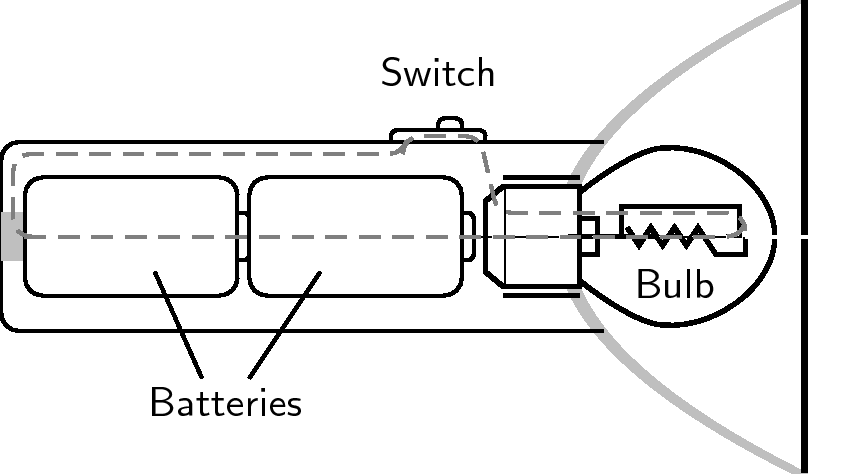
\includegraphics{col11305.imgs/m38516_PG10C9_009.png} % m38771;PG10C9\_009.png;;;6.0;8.5;
        
      \vspace{2pt}
    \vspace{\rubberspace}\par \begin{cnxcaption}
	  \small \textbf{Figure 16.9: }Physical components of an electric torch. The dotted line shows the path of the electrical circuit.
	\end{cnxcaption}
      
    \vspace{.1in}
    \rule[.1in]{\figurerulewidth}{.005in} \\
        
    \end{center}

 \end{figure}   

    \addtocounter{footnote}{-0}
    
          \label{m38771*id63252}Below is the \textsl{circuit diagram} for the electric torch. Now the light bulb is represented by its symbol, as are the batteries, the switch and the connecting wires. It is not necessary to show the plastic casing of the torch since it has nothing to do with the electric workings of the torch. You can see that the circuit diagram is much simpler than the physical circuit drawing!\par 
          
    \setcounter{subfigure}{0}


	\begin{figure}[H] % horizontal\label{m38771*uid15}
    \begin{center}
    \rule[.1in]{\figurerulewidth}{.005in} \\
        \label{m38771*uid15!!!underscore!!!media}\label{m38771*uid15!!!underscore!!!printimage}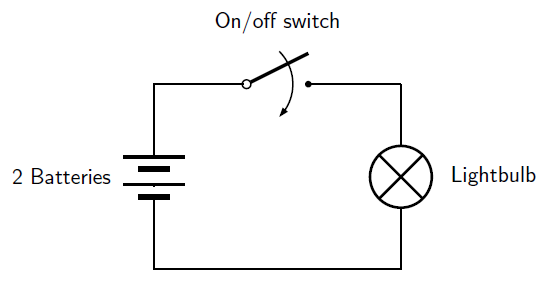
\includegraphics[width=300px]{col11305.imgs/m38516_PG10C9_010.png} % m38771;PG10C9\_010.png;;;6.0;8.5;
        
      \vspace{2pt}
    \vspace{\rubberspace}\par \begin{cnxcaption}
	  \small \textbf{Figure 16.10: }Circuit diagram of an electric torch.
	\end{cnxcaption}
      
    \vspace{.1in}
    \rule[.1in]{\figurerulewidth}{.005in} \\
        
    \end{center}

 \end{figure}   

    \addtocounter{footnote}{-0}
    
        
        \label{m38771*uid16}
            \subsubsection{ Series and parallel circuits}
            \nopagebreak
            
          
          \label{m38771*id63292}There are two ways to connect electrical components in a circuit: \textbf{in series} or \textbf{in parallel}.\par 
\label{m38771*fhsst!!!underscore!!!id283}\begin{definition}
	  \begin{tabular*}{15 cm}{m{15 mm}m{}}
	\hspace*{-50pt}  
\includegraphics[width=0.5in]{col11305.imgs/psflag2.png}   & \Definition{   \label{id2478736}\textbf{ Series circuit }} { \label{m38771*meaningfhsst!!!underscore!!!id283}
          \label{m38771*id63313}In a series circuit, the charge flowing from the battery can only flow along a \textbf{single} path to return to the battery. \par 
           } 
      \end{tabular*}
      \end{definition}

\label{m38771*fhsst!!!underscore!!!id286}\begin{definition}
	  \begin{tabular*}{15 cm}{m{15 mm}m{}}
	\hspace*{-50pt}  
\includegraphics[width=0.5in]{col11305.imgs/psflag2.png}   & \Definition{   \label{id2478767}\textbf{ Parallel circuit }} { \label{m38771*meaningfhsst!!!underscore!!!id286}
          \label{m38771*id63335}In a parallel circuit, the charge flowing from the battery can flow along \textbf{multiple} paths to return to the battery. \par 
           } 
      \end{tabular*}
      \end{definition}

          \label{m38771*id63352}The picture below shows a circuit with two resistors connected \textsl{in series} on the left and a circuit with two resistors connected \textsl{in parallel} on the right. In the series circiut, the charge path from the battery goes through every component before returning to the battery. In the parallel circuit, there is more than one path for the charge to flow from the battery through one of the components and back to the battery.\par 
          \label{m38771*id63369}
            
    \setcounter{subfigure}{0}


	\begin{figure}[H] % horizontal\label{m38771*id63372}
    \begin{center}
    \label{m38771*id63372!!!underscore!!!media}\label{m38771*id63372!!!underscore!!!printimage}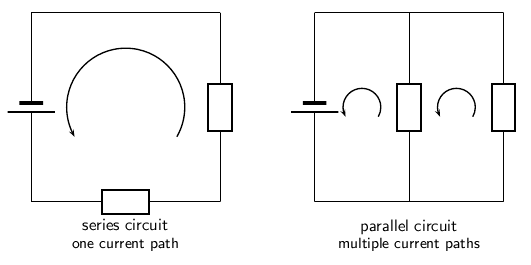
\includegraphics[width=300px]{col11305.imgs/m38771_PG11C9_006.png} % m38771;PG11C9\_006.png;;;6.0;8.5;
        
      \vspace{2pt}
    \vspace{.1in}
    
    \end{center}

 \end{figure}   

    \addtocounter{footnote}{-0}
    
          \par 

\label{m38771*fs-id5490818}This simulation allows you to experiment with building circuits.
 \raisebox{-5 pt}{ 
\includegraphics[width=0.5cm]{col11305.imgs/summary_www.png}} {(Simulation: lbK)}





\par
            \label{m38771*secfhsst!!!underscore!!!id298}\vspace{.5cm} 
      
      \noindent
      \hspace*{-30pt}
\includegraphics[width=0.5in]{col11305.imgs/pspencil2.png}   \raisebox{25mm}{   
      \begin{mdframed}[linewidth=4, leftmargin=40, rightmargin=40]  
      \begin{exercise}
    \noindent\textbf{Exercise 16.1:  Drawing circuits I }
          \label{m38771*probfhsst!!!underscore!!!id299}
          \label{m38771*id63390}Draw the circuit diagram for a circuit which has the following components:\par 
          \label{m38771*id63396}\begin{enumerate}[noitemsep, label=\textbf{\arabic*}. ] 
            \leftskip=20pt\rightskip=\leftskip\label{m38771*uid17}\item 1 battery
\label{m38771*uid18}\item 1 lightbulb connected in series
\label{m38771*uid19}\item 2 resistors connected in parallel
\end{enumerate}
        
          
          \vspace{5pt}
          \label{m38771*solfhsst!!!underscore!!!id311}\noindent\textbf{Solution to Exercise } \label{m38771*listfhsst!!!underscore!!!id311}\begin{enumerate}[noitemsep, label=\textbf{Step} \textbf{\arabic*}. ] 
            \leftskip=20pt\rightskip=\leftskip\item  
          \label{m38771*id63455}
            
    \setcounter{subfigure}{0}


	\begin{figure}[H] % horizontal\label{m38771*id63458}
    \begin{center}
    \label{m38771*id63458!!!underscore!!!media}\label{m38771*id63458!!!underscore!!!printimage}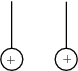
\includegraphics{col11305.imgs/m38771_PG10C9_012.png} % ;PG10C9\_012.png;;;6.0;8.5;
        
      \vspace{2pt}
    \vspace{.1in}
    
    \end{center}

 \end{figure}   

    \addtocounter{footnote}{-0}
    
          \par 
          
          \end{enumerate}
         

    \end{exercise}
    \end{mdframed}
    }
    \noindent
  
\label{m38771*secfhsst!!!underscore!!!id324}\vspace{.5cm} 
      
      \noindent
      \hspace*{-30pt}
\includegraphics[width=0.5in]{col11305.imgs/pspencil2.png}   \raisebox{25mm}{   
      \begin{mdframed}[linewidth=4, leftmargin=40, rightmargin=40]  
      \begin{exercise}
    \noindent\textbf{Exercise 16.2:  Drawing circuits II }
          \label{m38771*probfhsst!!!underscore!!!id325}
          \label{m38771*id63490}Draw the circuit diagram for a circuit which has the following components:\par 
          \label{m38771*id63497}\begin{enumerate}[noitemsep, label=\textbf{\arabic*}. ] 
            \leftskip=20pt\rightskip=\leftskip\label{m38771*uid20}\item 3 batteries in series
\label{m38771*uid21}\item 1 lightbulb connected in parallel with 1 resistor
\label{m38771*uid22}\item a switch in series with the batteries
\end{enumerate}
        
          
          \vspace{5pt}
          \label{m38771*solfhsst!!!underscore!!!id337}\noindent\textbf{Solution to Exercise } \label{m38771*listfhsst!!!underscore!!!id337}\begin{enumerate}[noitemsep, label=\textbf{Step} \textbf{\arabic*}. ] 
            \leftskip=20pt\rightskip=\leftskip\item  
          \label{m38771*id63560}
            
    \setcounter{subfigure}{0}


	\begin{figure}[H] % horizontal\label{m38771*id63563}
    \begin{center}
    \label{m38771*id63563!!!underscore!!!media}\label{m38771*id63563!!!underscore!!!printimage}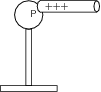
\includegraphics{col11305.imgs/m38771_PG10C9_013.png} % ;PG10C9\_013.png;;;6.0;8.5;
        
      \vspace{2pt}
    \vspace{.1in}
    
    \end{center}

 \end{figure}   

    \addtocounter{footnote}{-0}
    
          \par 
          
          \end{enumerate}
         

    \end{exercise}
    \end{mdframed}
    }
    \noindent
  
\label{m38771*secfhsst!!!underscore!!!id350}
            \subsubsection{  Circuits }
            \nopagebreak
            
          \label{m38771*id63592}\begin{enumerate}[noitemsep, label=\textbf{\arabic*}. ] 
            \label{m38771*uid23}\item Using physical components, set up the physical circuit which is described by the circuit diagram below and then draw the physical circuit:

    \setcounter{subfigure}{0}


	\begin{figure}[H] % horizontal\label{m38771*id63611}
    \begin{center}
    \label{m38771*id63611!!!underscore!!!media}\label{m38771*id63611!!!underscore!!!printimage}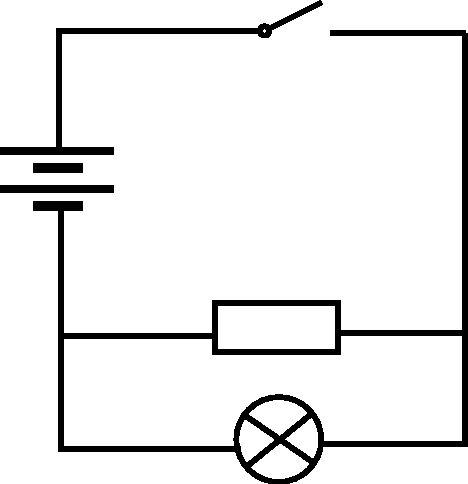
\includegraphics{col11305.imgs/m38771_PG10C9_014.png} % m38771;PG10C9\_014.png;;;6.0;8.5;
        
      \vspace{2pt}
    \vspace{.1in}
    
    \end{center}

 \end{figure}   

    \addtocounter{footnote}{-0}
     
         \label{m38771*uid24}\item Using physical components, set up a closed circuit which has one battery and a light bulb in series with a resistor.
\label{m38771*id63631}\begin{enumerate}[noitemsep, label=\textbf{\alph*}. ] 
            \label{m38771*uid25}\item Draw the physical circuit.
\label{m38771*uid26}\item Draw the resulting circuit diagram.
\label{m38771*uid27}\item How do you know that you have built a closed circuit? (What happens to the light bulb?)
\label{m38771*uid28}\item If you add one more resistor to your circuit (also in series), what do you notice? (What happens to the light from the light bulb?)
\label{m38771*uid29}\item Draw the new circuit diagram which includes the second resistor.
\end{enumerate}
                    \label{m38771*uid30}\item Draw the circuit diagram for the following circuit: 2 batteries and a switch in series, and 1 lightbulb which is in parallel with two resistors.
\label{m38771*id63711}\begin{enumerate}[noitemsep, label=\textbf{\alph*}. ] 
            \label{m38771*uid31}\item Now use physical components to set up the circuit.
\label{m38771*uid32}\item What happens when you close the switch? What does does this mean about the circuit?
\label{m38771*uid33}\item Draw the physical circuit.
\end{enumerate}
                  \end{enumerate}
        
          

\label{m38771*secfhsst!!!underscore!!!id369}
\par \raisebox{-5 pt}{
\includegraphics[width=0.5cm]{col11305.imgs/summary_www.png}} Find the answers with the shortcodes:
 \par \begin{tabular}[h]{cccccc}
 (1.) lqZ  &  (2.) lqB  &  (3.) lbY  & \end{tabular}



            \subsubsection{ Discussion : Alternative Energy }
            \nopagebreak
            \label{m38771*id63771}At the moment, most electric power is produced by burning fossil fuels such as coal and oil. In South Africa, our main
source of electric power is coal-burning power stations. (We also have one nuclear power plant called Koeberg in the Western Cape). However, burning fossil fuels releases large amounts of pollution into the earth's atmosphere and contributes
to global warming. Also, the earth's fossil fuel reserves (especially oil) are starting to run low. For these reasons, people all across the world are working to find \textsl{alternative}/other sources of energy and on ways to \textsl{conserve}/save energy. Other sources of energy include
wind power, solar power (from the sun), and hydro-electric power (from water, e.g. dammed rivers) among others.\par 
          \label{m38771*id63794}With a partner, take out the lists you made earlier of the item/appliances/machines which used electricity in the following environments. For each item, try to think of an \textsl{alternative} AND a way to \textsl{conserve} or save power.\par 
          \label{m38771*id63812}For example, if you had a flourescent light as an item used in the home, then:\par 
          \label{m38771*id63819}\begin{itemize}[noitemsep]
            \label{m38771*uid34}\item Alternative: use candles at suppertime to reduce electricity consumption
\label{m38771*uid35}\item Conservation: turn off lights when not in a room, or during the day.
\end{itemize}
        
          \label{m38771*id63848}
            \textbf{Topics:}
          \par 
          \label{m38771*id63857}\begin{itemize}[noitemsep]
            \label{m38771*uid36}\item At home
\label{m38771*uid37}\item At school
\label{m38771*uid38}\item At the hospital
\label{m38771*uid39}\item In the city
\end{itemize}
        
          \label{m38771*id63910}Once you have finished making your lists, compare with the lists of other people in your class.
 \par 

        
      
    

  \label{m38771**end}
          
         \section{ Potential difference}
    \nopagebreak
            \label{m38772} $ \hspace{-5pt}\begin{array}{cccccccccccc}   
\includegraphics[width=0.75cm]{col11305.imgs/summary_fullmarks.png} &   \end{array} $ \hspace{2 pt}\raisebox{-5 pt}{} {(section shortcode: P10075 )} \par 
    
    
    
    
    
    
  
    \label{m38772*cid3}
            \subsection{ Potential Difference}
            \nopagebreak
            
      
      \label{m38772*uid40}
            \subsubsection{ Potential Difference}
            \nopagebreak
            
        
        \label{m38772*id63941}When a circuit is connected and complete, charge can move through the circuit. Charge will not move unless there is something to make it move. Think of it as though charge is at rest and something has to push it along. This means that work needs to be done to make charge move. A force acts on the charges, doing work, to make them move. The force is provided by the battery in the circuit.\par 
        \label{m38772*id63948}We call the moving charge "current" and we will talk about this later.\par 
        
        \label{m38772*id63957}The amount of work done to move a unit charge from one point to another point in a circuit is called the potential difference between those two points. You can think of it as a difference in the potential energy of the unit charge due to its position in the circuit. The difference in potential energy, called potential difference, is equal to the amount of work done to move the unit charge between the two points. Just like with gravity, when you raise an object above the ground it has gravitational potential energy due to its position, the same goes for a charge in a circuit and electrical potential energy. Potential difference is measured \textsl{between} or \textsl{across} two points. We do not say potential difference \textsl{through} something.\par 
\label{m38772*fhsst!!!underscore!!!id409}\begin{definition}
	  \begin{tabular*}{15 cm}{m{15 mm}m{}}
	\hspace*{-50pt}  
\includegraphics[width=0.5in]{col11305.imgs/psflag2.png}   & \Definition{   \label{id2479718}\textbf{ Potential Difference }} { \label{m38772*meaningfhsst!!!underscore!!!id409}
        \label{m38772*id63970}Electrical potential difference is the difference in electrical potential energy per unit charge between two points. The unit of potential difference is the volt\label{m38772*uid41}\footnote{named after the Italian physicist Alessandro Volta (1745--1827)} (V). 
The potential difference of a battery is the voltage measured across it when current is flowing through it.
\par 
         } 
      \end{tabular*}
      \end{definition}

        \label{m38772*id63994}The unit of potential difference is the volt (V), which is the same as 1 joule per coulomb, the amount of work done per unit charge. Electrical potential difference is also called voltage.\par 
      

      \label{m38772*s1}
            \subsubsection{ Potential difference and emf}
            \nopagebreak
            
	
	\label{m38772*sp1}
	  We use an instrument called a voltmeter to measure the potential difference between two points in a circuit. It must be connected across the two points, \textsl{in parallel} to that portion of the circuit as shown in the diagram below.
	\par   
        
    \setcounter{subfigure}{0}


	\begin{figure}[H] % horizontal\label{m38772*uid73s1}
    \begin{center}
    \rule[.1in]{\figurerulewidth}{.005in} \\
        \label{m38772*uid73s1!!!underscore!!!media}\label{m38772*uid73s1!!!underscore!!!printimage}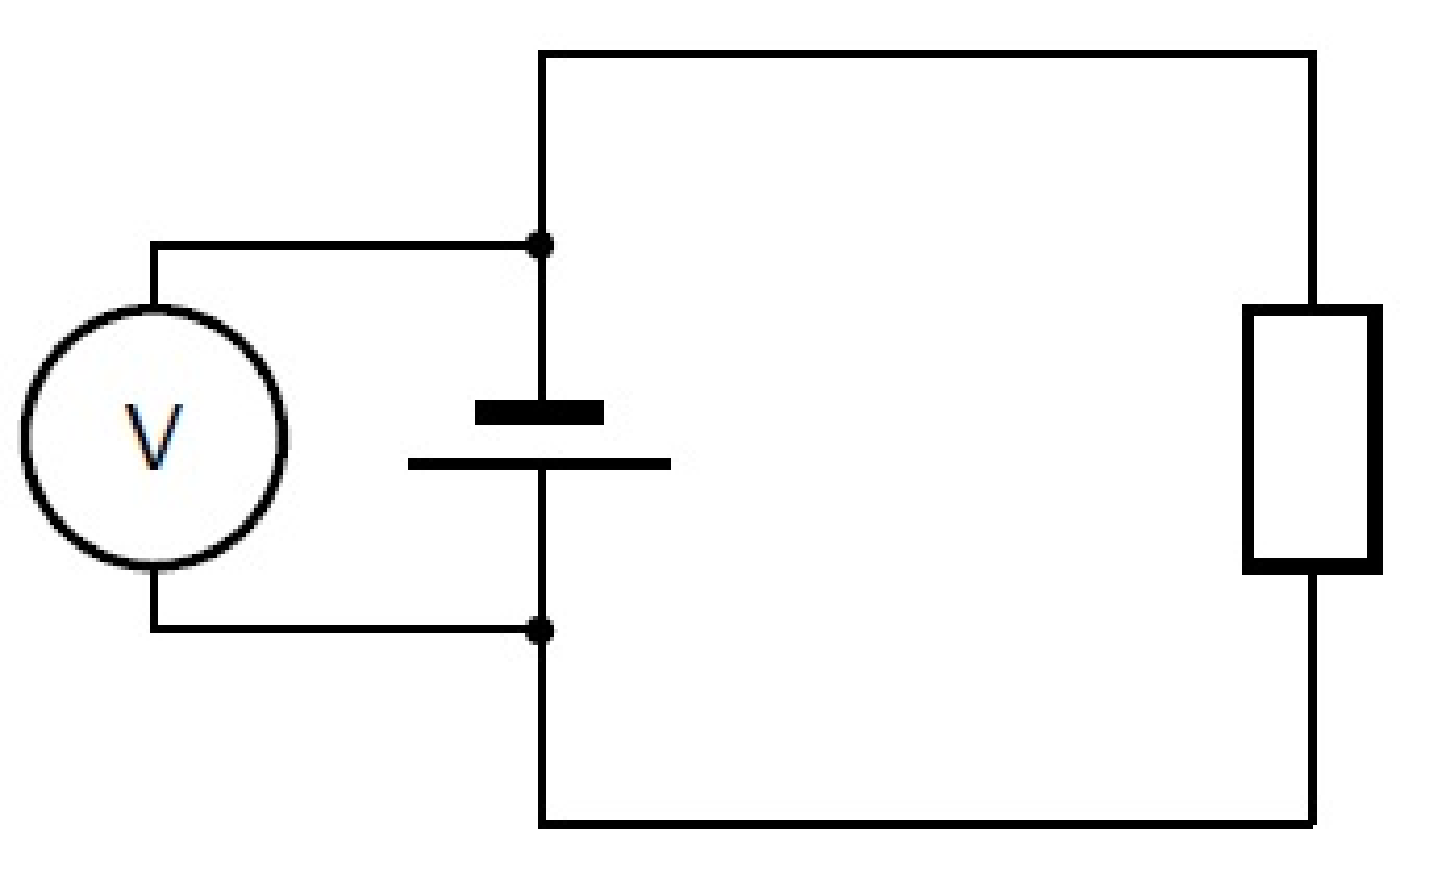
\includegraphics[width=0.4\columnwidth]{col11305.imgs/m38772_PG10C9_034.png} % m38772;PG10C9\_034.png;;;6.0;8.5;
        
      \vspace{2pt}
    \vspace{\rubberspace}\par \begin{cnxcaption}
	  \small \textbf{Figure 16.16: }A voltmeter should be connected in parallel in a circuit.
	\end{cnxcaption}
      
    \vspace{.1in}
    \rule[.1in]{\figurerulewidth}{.005in} \\
        
    \end{center}

 \end{figure}   

    \addtocounter{footnote}{-0}
    
      \label{m38772*uid45}
            \subsubsection{ EMF}
            \nopagebreak
            
        
        \label{m38772*id64666}When you use a voltmeter to measure the potential difference across (or between) the terminals of a battery, when no current is flowing through the battery, you are measuring the \textbf{electromotive force (emf)} of the battery. This is how much potential energy the battery has to make charges move through the circuit. It is a measure of how much chemical potential energy can be transferred to electrical energy in the battery. This driving potential energy is equal to the total potential energy drops in the circuit. This means that the voltage across the battery is equal to the sum of the voltages in the circuit.

\vspace{\rubberspace}\par
        \label{m38772*emf}\begin{definition}
	  \begin{tabular*}{15 cm}{m{15 mm}m{}}
	\hspace*{-50pt}  
\includegraphics[width=0.5in]{col11305.imgs/psflag2.png}   & \Definition{   \label{id2479864}\textbf{emf}} { \label{m38772*emf1meaning}
The emf (electromotive force) is the voltage measured across the terminals of a battery when \textsl{no current is flowing} through the battery.
 } 
      \end{tabular*}
      \end{definition}
\par 

	\label{m38772*ffgfgfgf}
	  You have now learnt that the emf is the voltage measured across the terminals of a battery when there is no current flowing through it and that the potential difference of a battery is the voltage measured across it when there is current flowing through it. So how do these two quantities compare with each other? 
	\par   

	\label{m38772*secfhsst!!!underscore!!!id1616s1}
            \subsubsection{ Experiment : Investigate the emf and potential difference of a battery }
            \nopagebreak
            
	  \label{m38772*parasar1}\noindent{}\textbf{Aim:} To measure the emf and potential difference across a battery in a circuit\par 
	  \label{m38772*parasar11}\noindent{}\textbf{Apparatus:} A battery, connecting wires, a light bulb, a switch, a voltmeter.\par 
	  \label{m38772*parasar111}\noindent{}\textbf{Method: } Set up a circuit with a battery, a lightbulb and a switch connected in series.\par 
	       \label{m38772*parasar11111}First we will measure the emf of the battery when no current is flowing. Make sure that the switch is open and the lightbulb is not glowing. This is how we check that there is no current flowing through the circuit. Then connect the voltmeter across the terminals of the battery. Make sure that the voltmeter is set to the largest scale when you first start measuring. Write down the voltage you measure. This is the emf. Disconnect the voltmeter.\par 
	       \label{m38772*parasar15}Second we will measure the potential difference across the battery. This time, make sure the switch is closed and that the lightbulb is glowing. This means that there is current flowing through the circuit. Now connect the voltmeter again across the terminals of the battery. Again make sure that the voltmeter is set on its largest scale. Write down the voltage you measure. This is called the potential difference of the battery. How does it compare to the other value you measured when there was no current flowing?\par 
	  \label{m38772*parasar221}\noindent{}\textbf{Summary:}You will have noticed that the voltages you measured when there was no current flowing (emf) and when there was current flowing (potential difference) were different. The emf was a higher value than the potential difference. Discuss with your classmates and teacher why you think this might happen.\par 
	  

	\label{m38772*parasar13}
	  Batteries all have some internal resistance to charges moving through them and therefore some work is required to move the charges through the battery itself. This internal resistance causes the potential difference across the battery terminals to be slightly less than the emf. 
	\par   


        \label{m38772*id64677}In the following exercises, we will assume that we have 'perfect' batteries with no internal resistance. In this special case, the potential difference of the battery and its emf will be the same. We can use this information to solve problems in which the voltages across elements in a circuit add up to the emf.\par 
        \label{m38772*id64681}\nopagebreak\noindent{}
          \settowidth{\mymathboxwidth}{\begin{equation}
    EMF={V}_{total}\tag{16.1}
      \end{equation}
    }
    \typeout{Columnwidth = \the\columnwidth}\typeout{math as usual width = \the\mymathboxwidth}
    \ifthenelse{\lengthtest{\mymathboxwidth < \columnwidth}}{% if the math fits, do it again, for real
    \begin{equation}
    EMF={V}_{total}\tag{16.1}
      \end{equation}
    }{% else, if it doesn't fit
    \setlength{\mymathboxwidth}{\columnwidth}
      \addtolength{\mymathboxwidth}{-48pt}
    \par\vspace{12pt}\noindent\begin{minipage}{\columnwidth}
    \parbox[t]{\mymathboxwidth}{\large\begin{math}
    EMF={V}_{total}\end{math}}\hfill
    \parbox[t]{48pt}{\raggedleft 
    (16.1)}
    \end{minipage}\vspace{12pt}\par
    }% end of conditional for this bit of math
    \typeout{math as usual width = \the\mymathboxwidth}
    
        
\par
            \label{m38772*secfhsst!!!underscore!!!id616}\vspace{.5cm} 
     \vspace{\rubberspace} 
      \hspace*{-30pt}
\includegraphics[width=0.5in]{col11305.imgs/pspencil2.png}   \raisebox{25mm}{   
      \begin{mdframed}[linewidth=4, leftmargin=40, rightmargin=40]  
      \begin{exercise}
    \noindent\textbf{Exercise 16.3:  Voltages I }
        \label{m38772*probfhsst!!!underscore!!!id617}
        \label{m38772*id64727}What is the voltage across the resistor in the circuit shown?



    \setcounter{subfigure}{0}


	\begin{figure}[H] % horizontal\label{m38772*id64742}
    \begin{center}
    \label{m38772*id64742!!!underscore!!!media}\label{m38772*id64742!!!underscore!!!printimage}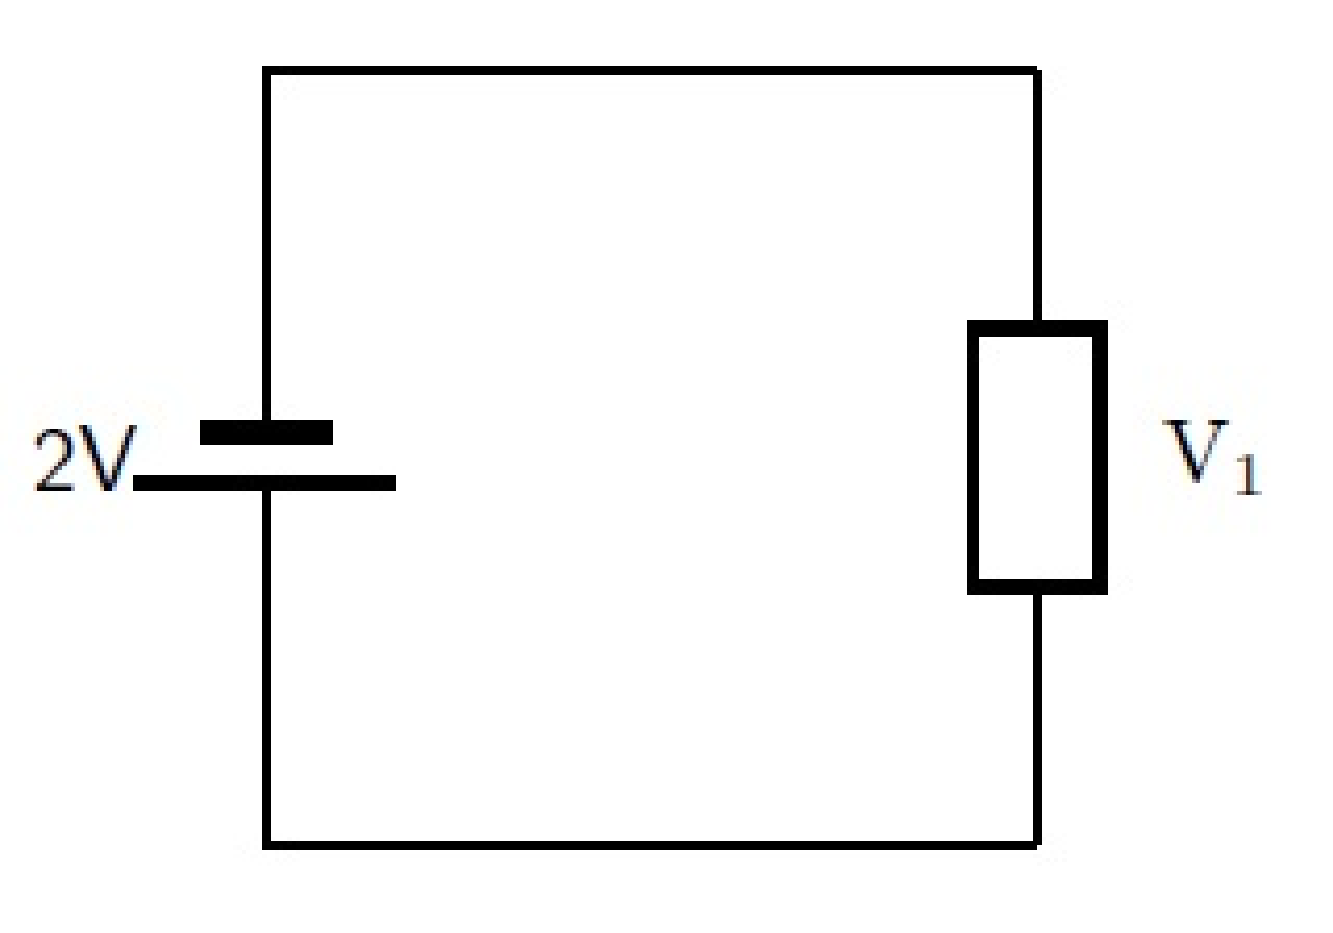
\includegraphics[width=0.4\columnwidth]{col11305.imgs/m38772_PG10C9_021.png} % m38772;PG10C9\_021.png;;;6.0;8.5;
        
      \vspace{2pt}
    \vspace{.1in}
    
    \end{center}

 \end{figure}   

    \addtocounter{footnote}{-0}
    


 \par 
        \vspace{5pt}
        \label{m38772*solfhsst!!!underscore!!!id626}\noindent\textbf{Solution to Exercise } \label{m38772*listfhsst!!!underscore!!!id626}\begin{enumerate}[noitemsep, label=\textbf{Step} \textbf{\arabic*}. ] 
            \leftskip=20pt\rightskip=\leftskip\item  
        \label{m38772*id64769}We have a circuit with a battery and one resistor. We know the voltage across the battery. We want to find the voltage across the resistor.\par 
        \label{m38772*id64773}\nopagebreak\noindent{}
          \settowidth{\mymathboxwidth}{\begin{equation}
    {V}_{battery}=2\mathrm{V}\tag{16.2}
      \end{equation}
    }
    \typeout{Columnwidth = \the\columnwidth}\typeout{math as usual width = \the\mymathboxwidth}
    \ifthenelse{\lengthtest{\mymathboxwidth < \columnwidth}}{% if the math fits, do it again, for real
    \begin{equation}
    {V}_{battery}=2\mathrm{V}\tag{16.2}
      \end{equation}
    }{% else, if it doesn't fit
    \setlength{\mymathboxwidth}{\columnwidth}
      \addtolength{\mymathboxwidth}{-48pt}
    \par\vspace{12pt}\noindent\begin{minipage}{\columnwidth}
    \parbox[t]{\mymathboxwidth}{\large\begin{math}
    {V}_{battery}=2\mathrm{V}\end{math}}\hfill
    \parbox[t]{48pt}{\raggedleft 
    (16.2)}
    \end{minipage}\vspace{12pt}\par
    }% end of conditional for this bit of math
    \typeout{math as usual width = \the\mymathboxwidth}
    
        
        \item  
        \label{m38772*id64817}We know that the voltage across the battery must be equal to the total voltage across all other circuit components.\par 
        \label{m38772*id64822}\nopagebreak\noindent{}
          \settowidth{\mymathboxwidth}{\begin{equation}
    {V}_{battery}={V}_{total}\tag{16.3}
      \end{equation}
    }
    \typeout{Columnwidth = \the\columnwidth}\typeout{math as usual width = \the\mymathboxwidth}
    \ifthenelse{\lengthtest{\mymathboxwidth < \columnwidth}}{% if the math fits, do it again, for real
    \begin{equation}
    {V}_{battery}={V}_{total}\tag{16.3}
      \end{equation}
    }{% else, if it doesn't fit
    \setlength{\mymathboxwidth}{\columnwidth}
      \addtolength{\mymathboxwidth}{-48pt}
    \par\vspace{12pt}\noindent\begin{minipage}{\columnwidth}
    \parbox[t]{\mymathboxwidth}{\large\begin{math}
    {V}_{battery}={V}_{total}\end{math}}\hfill
    \parbox[t]{48pt}{\raggedleft 
    (16.3)}
    \end{minipage}\vspace{12pt}\par
    }% end of conditional for this bit of math
    \typeout{math as usual width = \the\mymathboxwidth}
    
        
        \label{m38772*id64872}There is only one other circuit component, the resistor.\par 
        \label{m38772*id64878}\nopagebreak\noindent{}
          \settowidth{\mymathboxwidth}{\begin{equation}
    {V}_{total}={V}_{1}\tag{16.4}
      \end{equation}
    }
    \typeout{Columnwidth = \the\columnwidth}\typeout{math as usual width = \the\mymathboxwidth}
    \ifthenelse{\lengthtest{\mymathboxwidth < \columnwidth}}{% if the math fits, do it again, for real
    \begin{equation}
    {V}_{total}={V}_{1}\tag{16.4}
      \end{equation}
    }{% else, if it doesn't fit
    \setlength{\mymathboxwidth}{\columnwidth}
      \addtolength{\mymathboxwidth}{-48pt}
    \par\vspace{12pt}\noindent\begin{minipage}{\columnwidth}
    \parbox[t]{\mymathboxwidth}{\large\begin{math}
    {V}_{total}={V}_{1}\end{math}}\hfill
    \parbox[t]{48pt}{\raggedleft 
    (16.4)}
    \end{minipage}\vspace{12pt}\par
    }% end of conditional for this bit of math
    \typeout{math as usual width = \the\mymathboxwidth}
    
        
        \label{m38772*id64915}This means that the voltage across the battery is the same as the voltage across the resistor.\par 
        \label{m38772*id64921}\nopagebreak\noindent{}
          \settowidth{\mymathboxwidth}{\begin{equation}
    {V}_{battery}={V}_{total}={V}_{1}\tag{16.5}
      \end{equation}
    }
    \typeout{Columnwidth = \the\columnwidth}\typeout{math as usual width = \the\mymathboxwidth}
    \ifthenelse{\lengthtest{\mymathboxwidth < \columnwidth}}{% if the math fits, do it again, for real
    \begin{equation}
    {V}_{battery}={V}_{total}={V}_{1}\tag{16.5}
      \end{equation}
    }{% else, if it doesn't fit
    \setlength{\mymathboxwidth}{\columnwidth}
      \addtolength{\mymathboxwidth}{-48pt}
    \par\vspace{12pt}\noindent\begin{minipage}{\columnwidth}
    \parbox[t]{\mymathboxwidth}{\large\begin{math}
    {V}_{battery}={V}_{total}={V}_{1}\end{math}}\hfill
    \parbox[t]{48pt}{\raggedleft 
    (16.5)}
    \end{minipage}\vspace{12pt}\par
    }% end of conditional for this bit of math
    \typeout{math as usual width = \the\mymathboxwidth}
    
        
        \label{m38772*id64981}\nopagebreak\noindent{}
          \settowidth{\mymathboxwidth}{\begin{equation}
    {V}_{battery}={V}_{total}={V}_{1}\tag{16.6}
      \end{equation}
    }
    \typeout{Columnwidth = \the\columnwidth}\typeout{math as usual width = \the\mymathboxwidth}
    \ifthenelse{\lengthtest{\mymathboxwidth < \columnwidth}}{% if the math fits, do it again, for real
    \begin{equation}
    {V}_{battery}={V}_{total}={V}_{1}\tag{16.6}
      \end{equation}
    }{% else, if it doesn't fit
    \setlength{\mymathboxwidth}{\columnwidth}
      \addtolength{\mymathboxwidth}{-48pt}
    \par\vspace{12pt}\noindent\begin{minipage}{\columnwidth}
    \parbox[t]{\mymathboxwidth}{\large\begin{math}
    {V}_{battery}={V}_{total}={V}_{1}\end{math}}\hfill
    \parbox[t]{48pt}{\raggedleft 
    (16.6)}
    \end{minipage}\vspace{12pt}\par
    }% end of conditional for this bit of math
    \typeout{math as usual width = \the\mymathboxwidth}
    
        
        \label{m38772*id65041}\nopagebreak\noindent{}
          \settowidth{\mymathboxwidth}{\begin{equation}
    {V}_{1}=2\mathrm{V}\tag{16.7}
      \end{equation}
    }
    \typeout{Columnwidth = \the\columnwidth}\typeout{math as usual width = \the\mymathboxwidth}
    \ifthenelse{\lengthtest{\mymathboxwidth < \columnwidth}}{% if the math fits, do it again, for real
    \begin{equation}
    {V}_{1}=2\mathrm{V}\tag{16.7}
      \end{equation}
    }{% else, if it doesn't fit
    \setlength{\mymathboxwidth}{\columnwidth}
      \addtolength{\mymathboxwidth}{-48pt}
    \par\vspace{12pt}\noindent\begin{minipage}{\columnwidth}
    \parbox[t]{\mymathboxwidth}{\large\begin{math}
    {V}_{1}=2\mathrm{V}\end{math}}\hfill
    \parbox[t]{48pt}{\raggedleft 
    (16.7)}
    \end{minipage}\vspace{12pt}\par
    }% end of conditional for this bit of math
    \typeout{math as usual width = \the\mymathboxwidth}
    
        
        
        \end{enumerate}
         

    \end{exercise}
    \end{mdframed}
    }
    \noindent
  
\par
            \label{m38772*secfhsst!!!underscore!!!id788}\vspace{3.5cm} 
      \vspace{\rubberspace}
      \hspace*{-30pt}
\includegraphics[width=0.5in]{col11305.imgs/pspencil2.png}   \raisebox{25mm}{   
      \begin{mdframed}[linewidth=4, leftmargin=40, rightmargin=40]  
      \begin{exercise}
    \noindent\textbf{Exercise 16.4:  Voltages II }
        \label{m38772*probfhsst!!!underscore!!!id789}
        \label{m38772*id65094}What is the voltage across the unknown resistor in the circuit shown?



    \setcounter{subfigure}{0}


	\begin{figure}[H] % horizontal\label{m38772*id65109}
    \begin{center}
    \label{m38772*id65109!!!underscore!!!media}\label{m38772*id65109!!!underscore!!!printimage}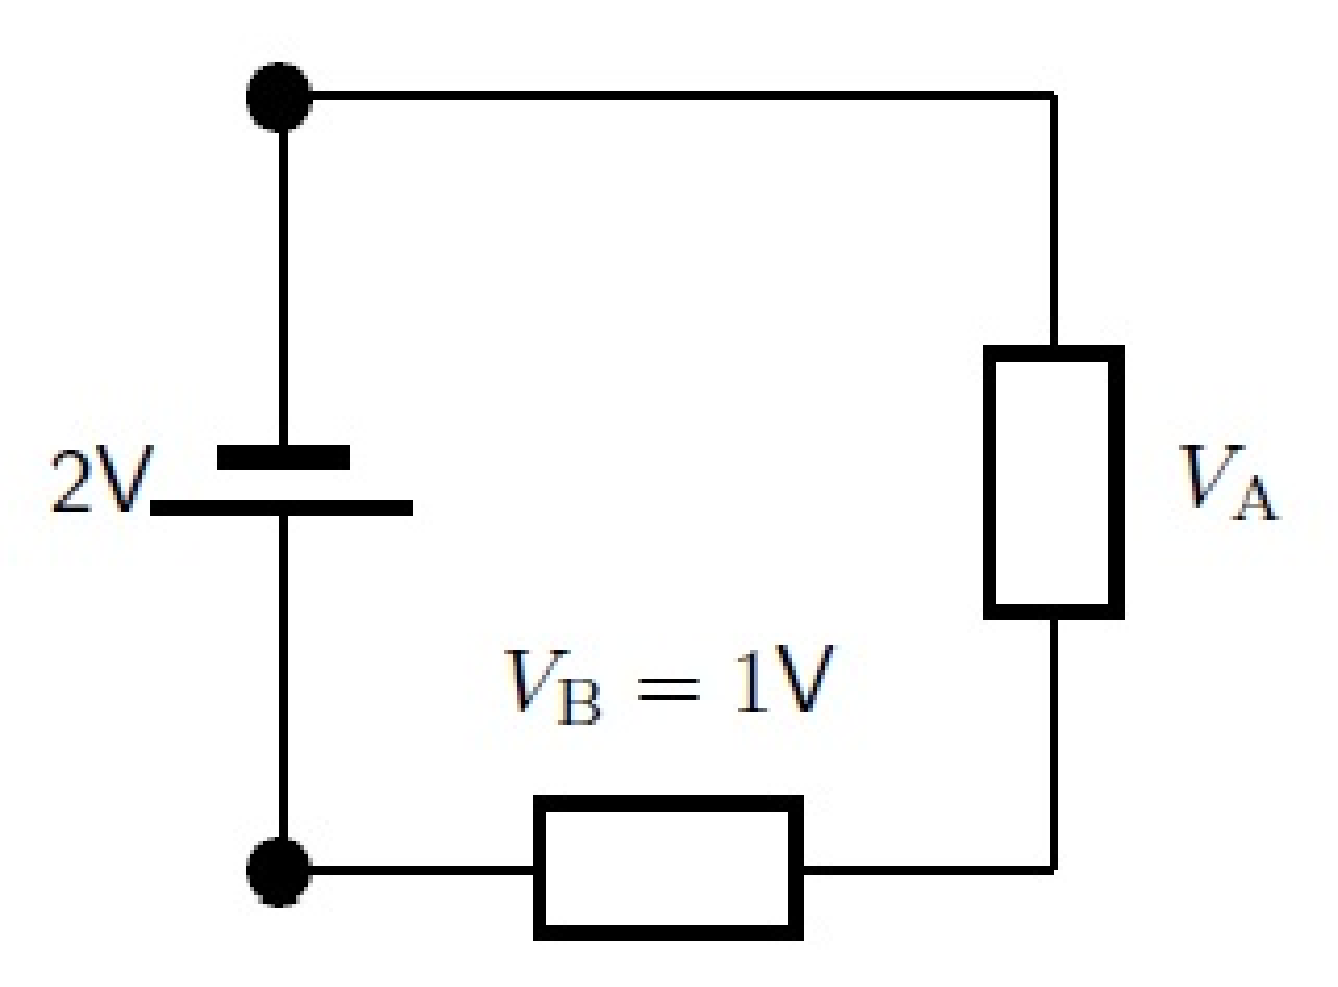
\includegraphics[width=0.4\columnwidth]{col11305.imgs/m38772_PG10C9_022.png} % m38772;PG10C9\_022.png;;;6.0;8.5;
        
      \vspace{2pt}
    \vspace{.1in}
    
    \end{center}

 \end{figure}   

    \addtocounter{footnote}{-0}
    


 \par 
        \vspace{5pt}
        \label{m38772*solfhsst!!!underscore!!!id798}\noindent\textbf{Solution to Exercise } \label{m38772*listfhsst!!!underscore!!!id798}\begin{enumerate}[noitemsep, label=\textbf{Step} \textbf{\arabic*}. ] 
            \leftskip=20pt\rightskip=\leftskip\item  
        \label{m38772*id65136}We have a circuit with a battery and two resistors. We know the voltage across the battery and one of the resistors. We want to find that voltage across the resistor.\par 
        \label{m38772*id65141}\nopagebreak\noindent{}
          \settowidth{\mymathboxwidth}{\begin{equation}
    {V}_{battery}=2\mathrm{V}\tag{16.8}
      \end{equation}
    }
    \typeout{Columnwidth = \the\columnwidth}\typeout{math as usual width = \the\mymathboxwidth}
    \ifthenelse{\lengthtest{\mymathboxwidth < \columnwidth}}{% if the math fits, do it again, for real
    \begin{equation}
    {V}_{battery}=2\mathrm{V}\tag{16.8}
      \end{equation}
    }{% else, if it doesn't fit
    \setlength{\mymathboxwidth}{\columnwidth}
      \addtolength{\mymathboxwidth}{-48pt}
    \par\vspace{12pt}\noindent\begin{minipage}{\columnwidth}
    \parbox[t]{\mymathboxwidth}{\large\begin{math}
    {V}_{battery}=2\mathrm{V}\end{math}}\hfill
    \parbox[t]{48pt}{\raggedleft 
    (16.8)}
    \end{minipage}\vspace{12pt}\par
    }% end of conditional for this bit of math
    \typeout{math as usual width = \the\mymathboxwidth}
    
        
        \label{m38772*id65181}\nopagebreak\noindent{}
          \settowidth{\mymathboxwidth}{\begin{equation}
    {V}_{\mathrm{A}}=1\mathrm{V}\tag{16.9}
      \end{equation}
    }
    \typeout{Columnwidth = \the\columnwidth}\typeout{math as usual width = \the\mymathboxwidth}
    \ifthenelse{\lengthtest{\mymathboxwidth < \columnwidth}}{% if the math fits, do it again, for real
    \begin{equation}
    {V}_{\mathrm{A}}=1\mathrm{V}\tag{16.9}
      \end{equation}
    }{% else, if it doesn't fit
    \setlength{\mymathboxwidth}{\columnwidth}
      \addtolength{\mymathboxwidth}{-48pt}
    \par\vspace{12pt}\noindent\begin{minipage}{\columnwidth}
    \parbox[t]{\mymathboxwidth}{\large\begin{math}
    {V}_{\mathrm{A}}=1\mathrm{V}\end{math}}\hfill
    \parbox[t]{48pt}{\raggedleft 
    (16.9)}
    \end{minipage}\vspace{12pt}\par
    }% end of conditional for this bit of math
    \typeout{math as usual width = \the\mymathboxwidth}
    
        
        \item  
        \label{m38772*id65213}We know that the voltage across the battery must be equal to the total voltage across all other circuit components that are in series.\par 
        \label{m38772*id65217}\nopagebreak\noindent{}
          \settowidth{\mymathboxwidth}{\begin{equation}
    {V}_{battery}={V}_{total}\tag{16.10}
      \end{equation}
    }
    \typeout{Columnwidth = \the\columnwidth}\typeout{math as usual width = \the\mymathboxwidth}
    \ifthenelse{\lengthtest{\mymathboxwidth < \columnwidth}}{% if the math fits, do it again, for real
    \begin{equation}
    {V}_{battery}={V}_{total}\tag{16.10}
      \end{equation}
    }{% else, if it doesn't fit
    \setlength{\mymathboxwidth}{\columnwidth}
      \addtolength{\mymathboxwidth}{-48pt}
    \par\vspace{12pt}\noindent\begin{minipage}{\columnwidth}
    \parbox[t]{\mymathboxwidth}{\large\begin{math}
    {V}_{battery}={V}_{total}\end{math}}\hfill
    \parbox[t]{48pt}{\raggedleft 
    (16.10)}
    \end{minipage}\vspace{12pt}\par
    }% end of conditional for this bit of math
    \typeout{math as usual width = \the\mymathboxwidth}
    
        
        \label{m38772*id65268}The total voltage in the circuit is the sum of the voltages across the individual resistors\par 
        \label{m38772*id65274}\nopagebreak\noindent{}
          \settowidth{\mymathboxwidth}{\begin{equation}
    {V}_{total}={V}_{\mathrm{A}}+{V}_{\mathrm{B}}\tag{16.11}
      \end{equation}
    }
    \typeout{Columnwidth = \the\columnwidth}\typeout{math as usual width = \the\mymathboxwidth}
    \ifthenelse{\lengthtest{\mymathboxwidth < \columnwidth}}{% if the math fits, do it again, for real
    \begin{equation}
    {V}_{total}={V}_{\mathrm{A}}+{V}_{\mathrm{B}}\tag{16.11}
      \end{equation}
    }{% else, if it doesn't fit
    \setlength{\mymathboxwidth}{\columnwidth}
      \addtolength{\mymathboxwidth}{-48pt}
    \par\vspace{12pt}\noindent\begin{minipage}{\columnwidth}
    \parbox[t]{\mymathboxwidth}{\large\begin{math}
    {V}_{total}={V}_{\mathrm{A}}+{V}_{\mathrm{B}}\end{math}}\hfill
    \parbox[t]{48pt}{\raggedleft 
    (16.11)}
    \end{minipage}\vspace{12pt}\par
    }% end of conditional for this bit of math
    \typeout{math as usual width = \the\mymathboxwidth}
    
        
        \label{m38772*id65325}Using the relationship between the voltage across the battery and total voltage across the resistors\par 
        \label{m38772*id65331}\nopagebreak\noindent{}
          \settowidth{\mymathboxwidth}{\begin{equation}
    {V}_{battery}={V}_{total}\tag{16.12}
      \end{equation}
    }
    \typeout{Columnwidth = \the\columnwidth}\typeout{math as usual width = \the\mymathboxwidth}
    \ifthenelse{\lengthtest{\mymathboxwidth < \columnwidth}}{% if the math fits, do it again, for real
    \begin{equation}
    {V}_{battery}={V}_{total}\tag{16.12}
      \end{equation}
    }{% else, if it doesn't fit
    \setlength{\mymathboxwidth}{\columnwidth}
      \addtolength{\mymathboxwidth}{-48pt}
    \par\vspace{12pt}\noindent\begin{minipage}{\columnwidth}
    \parbox[t]{\mymathboxwidth}{\large\begin{math}
    {V}_{battery}={V}_{total}\end{math}}\hfill
    \parbox[t]{48pt}{\raggedleft 
    (16.12)}
    \end{minipage}\vspace{12pt}\par
    }% end of conditional for this bit of math
    \typeout{math as usual width = \the\mymathboxwidth}
    
        
        \label{m38772*id65382}\nopagebreak\noindent{}
          \settowidth{\mymathboxwidth}{\begin{equation}
    \begin{array}{ccc}\hfill {V}_{battery}& =& {V}_{1}+{V}_{resistor}\hfill \\ \hfill 2\mathrm{V}& =& {V}_{1}+1\mathrm{V}\hfill \\ \hfill {V}_{1}& =& 1\mathrm{V}\hfill \end{array}\tag{16.13}
      \end{equation}
    }
    \typeout{Columnwidth = \the\columnwidth}\typeout{math as usual width = \the\mymathboxwidth}
    \ifthenelse{\lengthtest{\mymathboxwidth < \columnwidth}}{% if the math fits, do it again, for real
    \begin{equation}
    \begin{array}{ccc}\hfill {V}_{battery}& =& {V}_{1}+{V}_{resistor}\hfill \\ \hfill 2\mathrm{V}& =& {V}_{1}+1\mathrm{V}\hfill \\ \hfill {V}_{1}& =& 1\mathrm{V}\hfill \end{array}\tag{16.13}
      \end{equation}
    }{% else, if it doesn't fit
    \setlength{\mymathboxwidth}{\columnwidth}
      \addtolength{\mymathboxwidth}{-48pt}
    \par\vspace{12pt}\noindent\begin{minipage}{\columnwidth}
    \parbox[t]{\mymathboxwidth}{\large\begin{math}
    {V}_{battery}={V}_{1}+{V}_{resistor}2\mathrm{V}={V}_{1}+1\mathrm{V}{V}_{1}=1\mathrm{V}\end{math}}\hfill
    \parbox[t]{48pt}{\raggedleft 
    (16.13)}
    \end{minipage}\vspace{12pt}\par
    }% end of conditional for this bit of math
    \typeout{math as usual width = \the\mymathboxwidth}
    
        
        
        \end{enumerate}
         

    \end{exercise}
    \end{mdframed}
    }
    \noindent
  
\par
            \label{m38772*secfhsst!!!underscore!!!id1012}\vspace{.5cm} 
     \vspace{\rubberspace} 
      \hspace*{-30pt}
\includegraphics[width=0.5in]{col11305.imgs/pspencil2.png}   \raisebox{25mm}{   
      \begin{mdframed}[linewidth=4, leftmargin=40, rightmargin=40]  
      \begin{exercise}
    \noindent\textbf{Exercise 16.5:  Voltages III }
        \label{m38772*probfhsst!!!underscore!!!id1013}
        \label{m38772*id65553}What is the voltage across the unknown resistor in the circuit shown?



    \setcounter{subfigure}{0}


	\begin{figure}[H] % horizontal\label{m38772*id65568}
    \begin{center}
    \label{m38772*id65568!!!underscore!!!media}\label{m38772*id65568!!!underscore!!!printimage}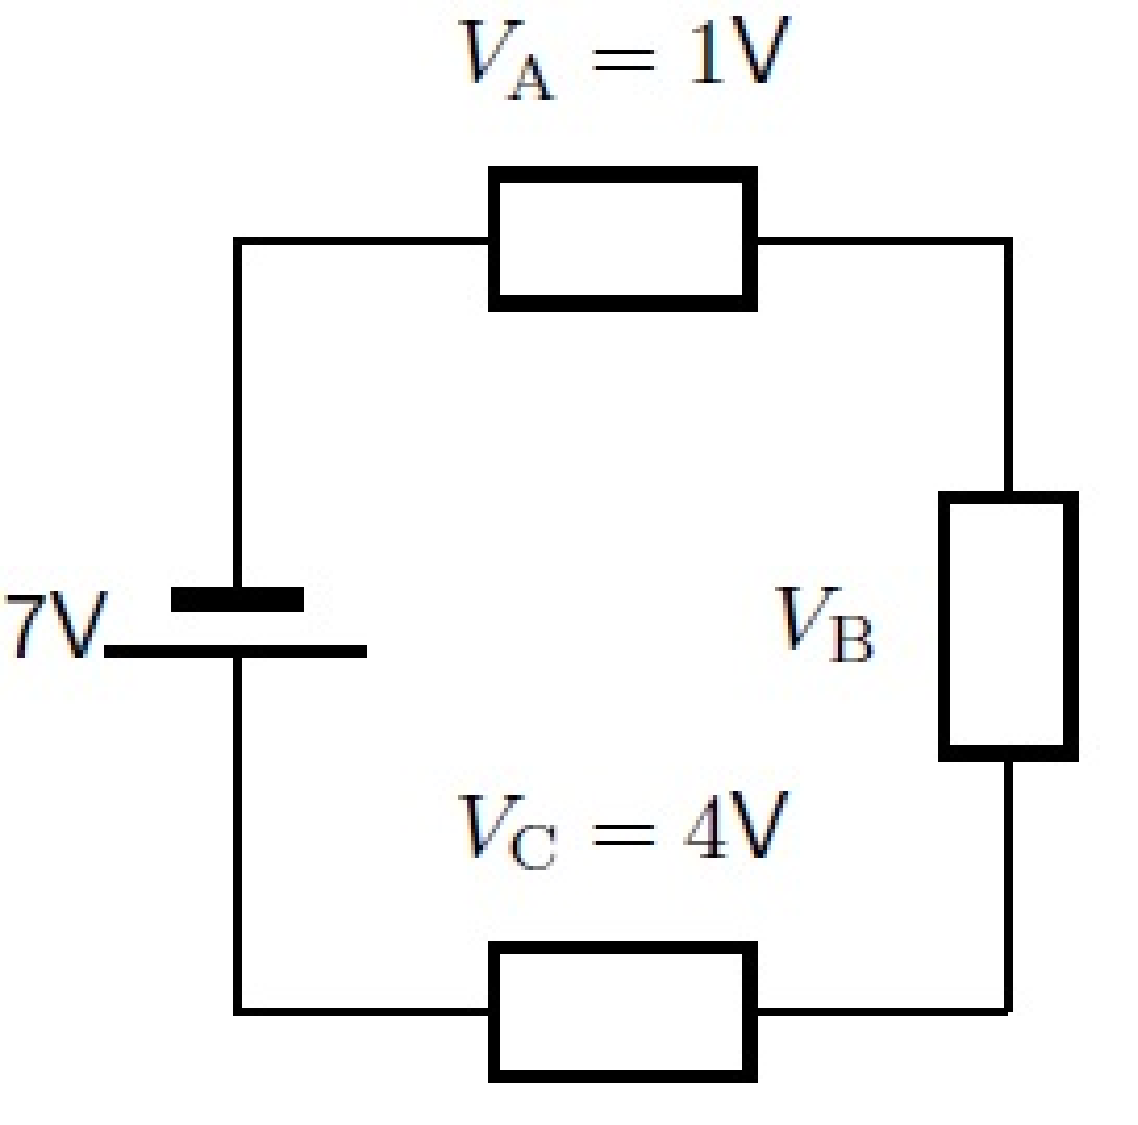
\includegraphics[width=0.4\columnwidth]{col11305.imgs/m38772_PG10C9_023.png} % m38772;PG10C9\_023.png;;;6.0;8.5;
        
      \vspace{2pt}
    \vspace{.1in}
    
    \end{center}

 \end{figure}   

    \addtocounter{footnote}{-0}
    


 \par 
        \vspace{5pt}
        \label{m38772*solfhsst!!!underscore!!!id1022}\noindent\textbf{Solution to Exercise } \label{m38772*listfhsst!!!underscore!!!id1022}\begin{enumerate}[noitemsep, label=\textbf{Step} \textbf{\arabic*}. ] 
            \leftskip=20pt\rightskip=\leftskip\item  
        \label{m38772*id65595}We have a circuit with a battery and three resistors. We know the voltage across the battery and two of the resistors. We want to find that voltage across the unknown resistor.\par 
        \label{m38772*id65600}\nopagebreak\noindent{}
          \settowidth{\mymathboxwidth}{\begin{equation}
    {V}_{battery}=7\mathrm{V}\tag{16.14}
      \end{equation}
    }
    \typeout{Columnwidth = \the\columnwidth}\typeout{math as usual width = \the\mymathboxwidth}
    \ifthenelse{\lengthtest{\mymathboxwidth < \columnwidth}}{% if the math fits, do it again, for real
    \begin{equation}
    {V}_{battery}=7\mathrm{V}\tag{16.14}
      \end{equation}
    }{% else, if it doesn't fit
    \setlength{\mymathboxwidth}{\columnwidth}
      \addtolength{\mymathboxwidth}{-48pt}
    \par\vspace{12pt}\noindent\begin{minipage}{\columnwidth}
    \parbox[t]{\mymathboxwidth}{\large\begin{math}
    {V}_{battery}=7\mathrm{V}\end{math}}\hfill
    \parbox[t]{48pt}{\raggedleft 
    (16.14)}
    \end{minipage}\vspace{12pt}\par
    }% end of conditional for this bit of math
    \typeout{math as usual width = \the\mymathboxwidth}
    
        
        \label{m38772*id65640}\nopagebreak\noindent{}
          \settowidth{\mymathboxwidth}{\begin{equation}
    \begin{array}{ccc}\hfill {V}_{known}& =& {V}_{\mathrm{A}}+{V}_{\mathrm{C}}\hfill \\ & =& 1\mathrm{V}+4\mathrm{V}\hfill \end{array}\tag{16.15}
      \end{equation}
    }
    \typeout{Columnwidth = \the\columnwidth}\typeout{math as usual width = \the\mymathboxwidth}
    \ifthenelse{\lengthtest{\mymathboxwidth < \columnwidth}}{% if the math fits, do it again, for real
    \begin{equation}
    \begin{array}{ccc}\hfill {V}_{known}& =& {V}_{\mathrm{A}}+{V}_{\mathrm{C}}\hfill \\ & =& 1\mathrm{V}+4\mathrm{V}\hfill \end{array}\tag{16.15}
      \end{equation}
    }{% else, if it doesn't fit
    \setlength{\mymathboxwidth}{\columnwidth}
      \addtolength{\mymathboxwidth}{-48pt}
    \par\vspace{12pt}\noindent\begin{minipage}{\columnwidth}
    \parbox[t]{\mymathboxwidth}{\large\begin{math}
    {V}_{known}={V}_{\mathrm{A}}+{V}_{\mathrm{C}}=1\mathrm{V}+4\mathrm{V}\end{math}}\hfill
    \parbox[t]{48pt}{\raggedleft 
    (16.15)}
    \end{minipage}\vspace{12pt}\par
    }% end of conditional for this bit of math
    \typeout{math as usual width = \the\mymathboxwidth}
    
        
        \item  
        \label{m38772*id65732}We know that the voltage across the battery must be equal to the total voltage across all other circuit components that are in series.\par 
        \label{m38772*id65736}\nopagebreak\noindent{}
          \settowidth{\mymathboxwidth}{\begin{equation}
    {V}_{battery}={V}_{total}\tag{16.16}
      \end{equation}
    }
    \typeout{Columnwidth = \the\columnwidth}\typeout{math as usual width = \the\mymathboxwidth}
    \ifthenelse{\lengthtest{\mymathboxwidth < \columnwidth}}{% if the math fits, do it again, for real
    \begin{equation}
    {V}_{battery}={V}_{total}\tag{16.16}
      \end{equation}
    }{% else, if it doesn't fit
    \setlength{\mymathboxwidth}{\columnwidth}
      \addtolength{\mymathboxwidth}{-48pt}
    \par\vspace{12pt}\noindent\begin{minipage}{\columnwidth}
    \parbox[t]{\mymathboxwidth}{\large\begin{math}
    {V}_{battery}={V}_{total}\end{math}}\hfill
    \parbox[t]{48pt}{\raggedleft 
    (16.16)}
    \end{minipage}\vspace{12pt}\par
    }% end of conditional for this bit of math
    \typeout{math as usual width = \the\mymathboxwidth}
    
        
        \label{m38772*id65787}The total voltage in the circuit is the sum of the voltages across the individual resistors\par 
        \label{m38772*id65794}\nopagebreak\noindent{}
          \settowidth{\mymathboxwidth}{\begin{equation}
    {V}_{total}={V}_{\mathrm{B}}+{V}_{known}\tag{16.17}
      \end{equation}
    }
    \typeout{Columnwidth = \the\columnwidth}\typeout{math as usual width = \the\mymathboxwidth}
    \ifthenelse{\lengthtest{\mymathboxwidth < \columnwidth}}{% if the math fits, do it again, for real
    \begin{equation}
    {V}_{total}={V}_{\mathrm{B}}+{V}_{known}\tag{16.17}
      \end{equation}
    }{% else, if it doesn't fit
    \setlength{\mymathboxwidth}{\columnwidth}
      \addtolength{\mymathboxwidth}{-48pt}
    \par\vspace{12pt}\noindent\begin{minipage}{\columnwidth}
    \parbox[t]{\mymathboxwidth}{\large\begin{math}
    {V}_{total}={V}_{\mathrm{B}}+{V}_{known}\end{math}}\hfill
    \parbox[t]{48pt}{\raggedleft 
    (16.17)}
    \end{minipage}\vspace{12pt}\par
    }% end of conditional for this bit of math
    \typeout{math as usual width = \the\mymathboxwidth}
    
        
        \label{m38772*id65851}Using the relationship between the voltage across the battery and total voltage across the resistors\par 
        \label{m38772*id65858}\nopagebreak\noindent{}
          \settowidth{\mymathboxwidth}{\begin{equation}
    {V}_{battery}={V}_{total}\tag{16.18}
      \end{equation}
    }
    \typeout{Columnwidth = \the\columnwidth}\typeout{math as usual width = \the\mymathboxwidth}
    \ifthenelse{\lengthtest{\mymathboxwidth < \columnwidth}}{% if the math fits, do it again, for real
    \begin{equation}
    {V}_{battery}={V}_{total}\tag{16.18}
      \end{equation}
    }{% else, if it doesn't fit
    \setlength{\mymathboxwidth}{\columnwidth}
      \addtolength{\mymathboxwidth}{-48pt}
    \par\vspace{12pt}\noindent\begin{minipage}{\columnwidth}
    \parbox[t]{\mymathboxwidth}{\large\begin{math}
    {V}_{battery}={V}_{total}\end{math}}\hfill
    \parbox[t]{48pt}{\raggedleft 
    (16.18)}
    \end{minipage}\vspace{12pt}\par
    }% end of conditional for this bit of math
    \typeout{math as usual width = \the\mymathboxwidth}
    
        
        \label{m38772*id65908}\nopagebreak\noindent{}
          \settowidth{\mymathboxwidth}{\begin{equation}
    \begin{array}{ccc}\hfill {V}_{battery}& =& {V}_{\mathrm{B}}+{V}_{known}\hfill \\ \hfill 7\mathrm{V}& =& {V}_{\mathrm{B}}+5\mathrm{V}\hfill \\ \hfill {V}_{\mathrm{B}}& =& 2\mathrm{V}\hfill \end{array}\tag{16.19}
      \end{equation}
    }
    \typeout{Columnwidth = \the\columnwidth}\typeout{math as usual width = \the\mymathboxwidth}
    \ifthenelse{\lengthtest{\mymathboxwidth < \columnwidth}}{% if the math fits, do it again, for real
    \begin{equation}
    \begin{array}{ccc}\hfill {V}_{battery}& =& {V}_{\mathrm{B}}+{V}_{known}\hfill \\ \hfill 7\mathrm{V}& =& {V}_{\mathrm{B}}+5\mathrm{V}\hfill \\ \hfill {V}_{\mathrm{B}}& =& 2\mathrm{V}\hfill \end{array}\tag{16.19}
      \end{equation}
    }{% else, if it doesn't fit
    \setlength{\mymathboxwidth}{\columnwidth}
      \addtolength{\mymathboxwidth}{-48pt}
    \par\vspace{12pt}\noindent\begin{minipage}{\columnwidth}
    \parbox[t]{\mymathboxwidth}{\large\begin{math}
    {V}_{battery}={V}_{\mathrm{B}}+{V}_{known}7\mathrm{V}={V}_{\mathrm{B}}+5\mathrm{V}{V}_{\mathrm{B}}=2\mathrm{V}\end{math}}\hfill
    \parbox[t]{48pt}{\raggedleft 
    (16.19)}
    \end{minipage}\vspace{12pt}\par
    }% end of conditional for this bit of math
    \typeout{math as usual width = \the\mymathboxwidth}
    
        
        
        \end{enumerate}
         

    \end{exercise}
    \end{mdframed}
    }
    \noindent
  
\par
            \label{m38772*secfhsst!!!underscore!!!id1277}\vspace{.5cm} 
      
      \noindent
      \hspace*{-30pt}
\includegraphics[width=0.5in]{col11305.imgs/pspencil2.png}   \raisebox{25mm}{   
      \begin{mdframed}[linewidth=4, leftmargin=40, rightmargin=40]  
      \begin{exercise}
    \noindent\textbf{Exercise 16.6:  Voltages IV }
        \label{m38772*probfhsst!!!underscore!!!id1278}
        \label{m38772*id66079}What is the voltage across the parallel resistor combination in the circuit shown? Hint: the rest of the circuit is the same as the previous problem.



    \setcounter{subfigure}{0}


	\begin{figure}[H] % horizontal\label{m38772*id66094}
    \begin{center}
    \label{m38772*id66094!!!underscore!!!media}\label{m38772*id66094!!!underscore!!!printimage}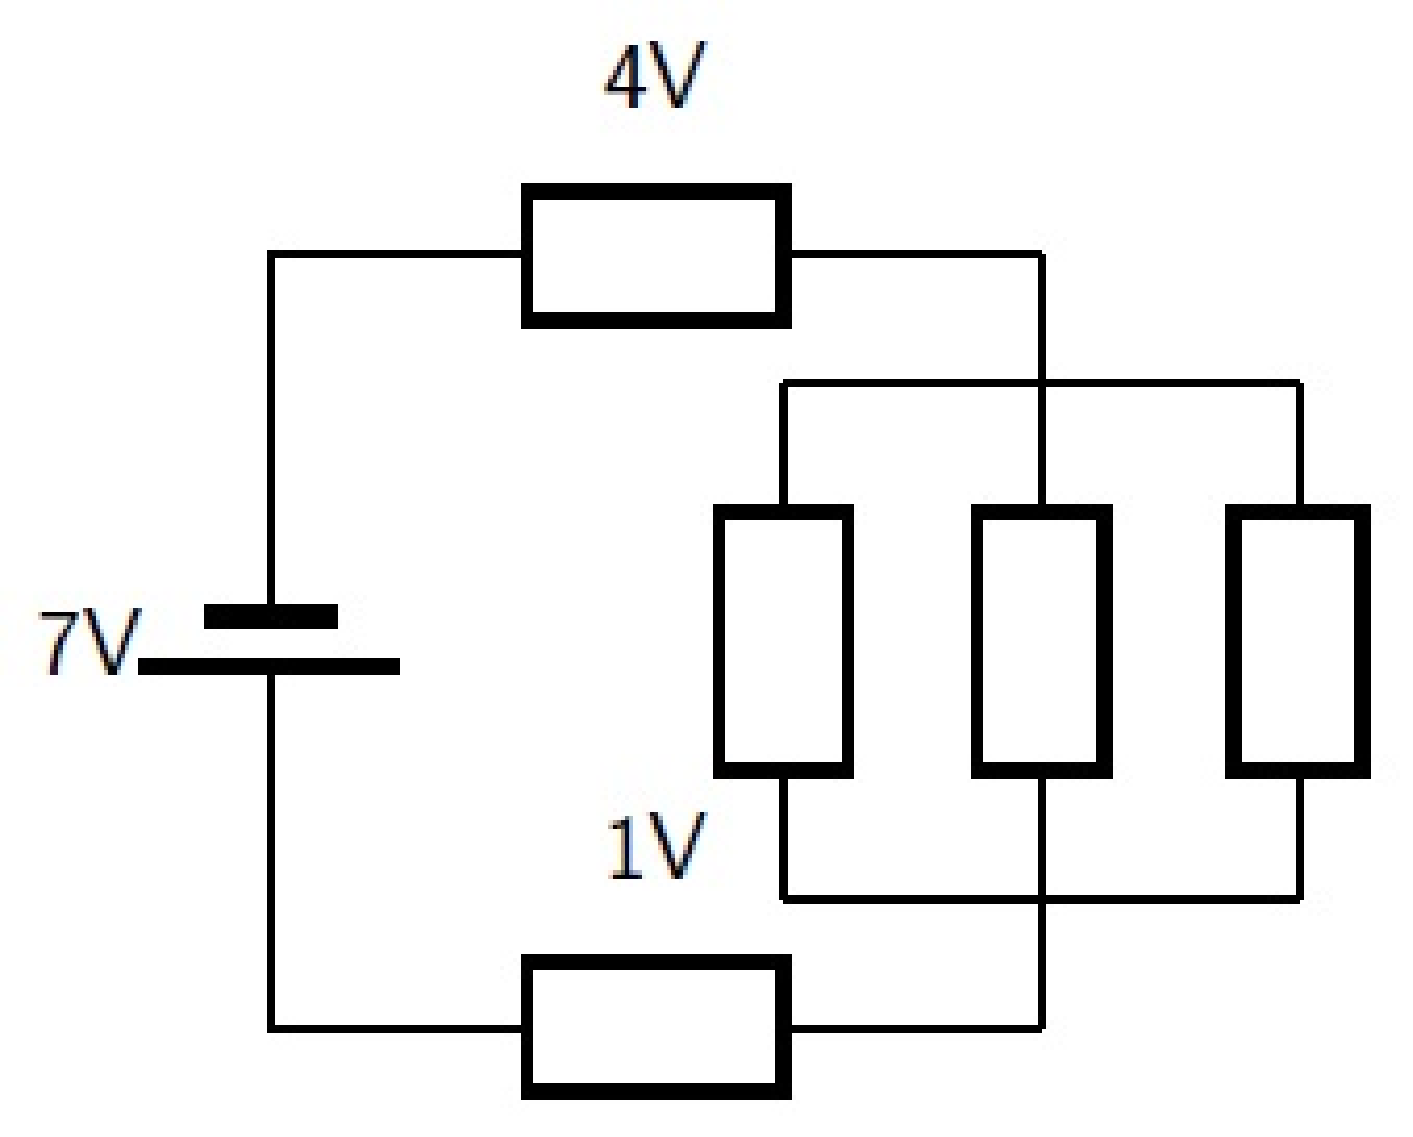
\includegraphics[width=0.4\columnwidth]{col11305.imgs/m38772_PG10C9_024.png} % m38772;PG10C9\_024.png;;;6.0;8.5;
        
      \vspace{2pt}
    \vspace{.1in}
    
    \end{center}

 \end{figure}   

    \addtocounter{footnote}{-0}
    


 \par 
        \vspace{5pt}
        \label{m38772*solfhsst!!!underscore!!!id1287}\noindent\textbf{Solution to Exercise } \label{m38772*listfhsst!!!underscore!!!id1287}\begin{enumerate}[noitemsep, label=\textbf{Step} \textbf{\arabic*}. ] 
            \leftskip=20pt\rightskip=\leftskip\item  
        \label{m38772*id66121}The circuit is the same as the previous example and we know that the voltage difference between two points in a circuit does not depend on what is between them so the answer is the same as above \begin{math}{V}_{parallel}=2\mathrm{V}\end{math}.\par 
        \item  
        \label{m38772*id66171}We have a circuit with a battery and five resistors (two in series and three in parallel). We know the voltage across the battery and two of the resistors. We want to find that voltage across the parallel resistors, \begin{math}{V}_{parallel}\end{math}.\par 
        \label{m38772*id66206}\nopagebreak\noindent{}
          \settowidth{\mymathboxwidth}{\begin{equation}
    {V}_{battery}=7\mathrm{V}\tag{16.20}
      \end{equation}
    }
    \typeout{Columnwidth = \the\columnwidth}\typeout{math as usual width = \the\mymathboxwidth}
    \ifthenelse{\lengthtest{\mymathboxwidth < \columnwidth}}{% if the math fits, do it again, for real
    \begin{equation}
    {V}_{battery}=7\mathrm{V}\tag{16.20}
      \end{equation}
    }{% else, if it doesn't fit
    \setlength{\mymathboxwidth}{\columnwidth}
      \addtolength{\mymathboxwidth}{-48pt}
    \par\vspace{12pt}\noindent\begin{minipage}{\columnwidth}
    \parbox[t]{\mymathboxwidth}{\large\begin{math}
    {V}_{battery}=7\mathrm{V}\end{math}}\hfill
    \parbox[t]{48pt}{\raggedleft 
    (16.20)}
    \end{minipage}\vspace{12pt}\par
    }% end of conditional for this bit of math
    \typeout{math as usual width = \the\mymathboxwidth}
    
        
        \label{m38772*id66245}\nopagebreak\noindent{}
          \settowidth{\mymathboxwidth}{\begin{equation}
    {V}_{known}=1\mathrm{V}+4\mathrm{V}\tag{16.21}
      \end{equation}
    }
    \typeout{Columnwidth = \the\columnwidth}\typeout{math as usual width = \the\mymathboxwidth}
    \ifthenelse{\lengthtest{\mymathboxwidth < \columnwidth}}{% if the math fits, do it again, for real
    \begin{equation}
    {V}_{known}=1\mathrm{V}+4\mathrm{V}\tag{16.21}
      \end{equation}
    }{% else, if it doesn't fit
    \setlength{\mymathboxwidth}{\columnwidth}
      \addtolength{\mymathboxwidth}{-48pt}
    \par\vspace{12pt}\noindent\begin{minipage}{\columnwidth}
    \parbox[t]{\mymathboxwidth}{\large\begin{math}
    {V}_{known}=1\mathrm{V}+4\mathrm{V}\end{math}}\hfill
    \parbox[t]{48pt}{\raggedleft 
    (16.21)}
    \end{minipage}\vspace{12pt}\par
    }% end of conditional for this bit of math
    \typeout{math as usual width = \the\mymathboxwidth}
    
        
        \item  
        \label{m38772*id66293}We know that the voltage across the battery must be equal to the total voltage across all other circuit components.\par 
        \label{m38772*id66297}\nopagebreak\noindent{}
          \settowidth{\mymathboxwidth}{\begin{equation}
    {V}_{battery}={V}_{total}\tag{16.22}
      \end{equation}
    }
    \typeout{Columnwidth = \the\columnwidth}\typeout{math as usual width = \the\mymathboxwidth}
    \ifthenelse{\lengthtest{\mymathboxwidth < \columnwidth}}{% if the math fits, do it again, for real
    \begin{equation}
    {V}_{battery}={V}_{total}\tag{16.22}
      \end{equation}
    }{% else, if it doesn't fit
    \setlength{\mymathboxwidth}{\columnwidth}
      \addtolength{\mymathboxwidth}{-48pt}
    \par\vspace{12pt}\noindent\begin{minipage}{\columnwidth}
    \parbox[t]{\mymathboxwidth}{\large\begin{math}
    {V}_{battery}={V}_{total}\end{math}}\hfill
    \parbox[t]{48pt}{\raggedleft 
    (16.22)}
    \end{minipage}\vspace{12pt}\par
    }% end of conditional for this bit of math
    \typeout{math as usual width = \the\mymathboxwidth}
    
        
        \label{m38772*id66348}Voltages only add for components in series. The resistors in parallel can be thought of as a single component which is in series with the other components and then the voltages can be added.\par 
        \label{m38772*id66355}\nopagebreak\noindent{}
          \settowidth{\mymathboxwidth}{\begin{equation}
    {V}_{total}={V}_{parallel}+{V}_{known}\tag{16.23}
      \end{equation}
    }
    \typeout{Columnwidth = \the\columnwidth}\typeout{math as usual width = \the\mymathboxwidth}
    \ifthenelse{\lengthtest{\mymathboxwidth < \columnwidth}}{% if the math fits, do it again, for real
    \begin{equation}
    {V}_{total}={V}_{parallel}+{V}_{known}\tag{16.23}
      \end{equation}
    }{% else, if it doesn't fit
    \setlength{\mymathboxwidth}{\columnwidth}
      \addtolength{\mymathboxwidth}{-48pt}
    \par\vspace{12pt}\noindent\begin{minipage}{\columnwidth}
    \parbox[t]{\mymathboxwidth}{\large\begin{math}
    {V}_{total}={V}_{parallel}+{V}_{known}\end{math}}\hfill
    \parbox[t]{48pt}{\raggedleft 
    (16.23)}
    \end{minipage}\vspace{12pt}\par
    }% end of conditional for this bit of math
    \typeout{math as usual width = \the\mymathboxwidth}
    
        
        \label{m38772*id66427}Using the relationship between the voltage across the battery and total voltage across the resistors\par 
        \label{m38772*id66433}\nopagebreak\noindent{}
          \settowidth{\mymathboxwidth}{\begin{equation}
    {V}_{battery}={V}_{total}\tag{16.24}
      \end{equation}
    }
    \typeout{Columnwidth = \the\columnwidth}\typeout{math as usual width = \the\mymathboxwidth}
    \ifthenelse{\lengthtest{\mymathboxwidth < \columnwidth}}{% if the math fits, do it again, for real
    \begin{equation}
    {V}_{battery}={V}_{total}\tag{16.24}
      \end{equation}
    }{% else, if it doesn't fit
    \setlength{\mymathboxwidth}{\columnwidth}
      \addtolength{\mymathboxwidth}{-48pt}
    \par\vspace{12pt}\noindent\begin{minipage}{\columnwidth}
    \parbox[t]{\mymathboxwidth}{\large\begin{math}
    {V}_{battery}={V}_{total}\end{math}}\hfill
    \parbox[t]{48pt}{\raggedleft 
    (16.24)}
    \end{minipage}\vspace{12pt}\par
    }% end of conditional for this bit of math
    \typeout{math as usual width = \the\mymathboxwidth}
    
        
        \label{m38772*id66483}\nopagebreak\noindent{}
          \settowidth{\mymathboxwidth}{\begin{equation}
    \begin{array}{ccc}\hfill {V}_{battery}& =& {V}_{parallel}+{V}_{known}\hfill \\ \hfill 7\mathrm{V}& =& {V}_{1}+5\mathrm{V}\hfill \\ \hfill {V}_{parallel}& =& 2\mathrm{V}\hfill \end{array}\tag{16.25}
      \end{equation}
    }
    \typeout{Columnwidth = \the\columnwidth}\typeout{math as usual width = \the\mymathboxwidth}
    \ifthenelse{\lengthtest{\mymathboxwidth < \columnwidth}}{% if the math fits, do it again, for real
    \begin{equation}
    \begin{array}{ccc}\hfill {V}_{battery}& =& {V}_{parallel}+{V}_{known}\hfill \\ \hfill 7\mathrm{V}& =& {V}_{1}+5\mathrm{V}\hfill \\ \hfill {V}_{parallel}& =& 2\mathrm{V}\hfill \end{array}\tag{16.25}
      \end{equation}
    }{% else, if it doesn't fit
    \setlength{\mymathboxwidth}{\columnwidth}
      \addtolength{\mymathboxwidth}{-48pt}
    \par\vspace{12pt}\noindent\begin{minipage}{\columnwidth}
    \parbox[t]{\mymathboxwidth}{\large\begin{math}
    {V}_{battery}={V}_{parallel}+{V}_{known}7\mathrm{V}={V}_{1}+5\mathrm{V}{V}_{parallel}=2\mathrm{V}\end{math}}\hfill
    \parbox[t]{48pt}{\raggedleft 
    (16.25)}
    \end{minipage}\vspace{12pt}\par
    }% end of conditional for this bit of math
    \typeout{math as usual width = \the\mymathboxwidth}
    
        
        
        \end{enumerate}
         

    \end{exercise}
    \end{mdframed}
    }
    \noindent
  
       

 
      












     

  \label{m38772**end}
          
         \section{ Current and measurement}
    \nopagebreak
            \label{m38773} $ \hspace{-5pt}\begin{array}{cccccccccccc}   
\includegraphics[width=0.75cm]{col11305.imgs/summary_fullmarks.png} &   \end{array} $ \hspace{2 pt}\raisebox{-5 pt}{} {(section shortcode: P10076 )} \par 
    
    
    
    
    
    
  
    \label{m38773*cid4}
            \subsection{ Current}
            \nopagebreak
            
      
      \label{m38773*uid46}
            \subsubsection{ Flow of Charge}
            \nopagebreak
            
        
        \label{m38773*id66684}We have been talking about moving charge. But how much charge is moving, and how fast is it moving? The concept that represents this information is called \textsl{current}. Current allows us to quantify the movement of charge.\par 
        \label{m38773*id66695}When we talk about current we talk about how much charge moves past a fixed point in circuit in one second. Think of charges being pushed around the circuit by the battery; there are charges in the wires but unless there is a battery they won't move. When one charge moves, the charges next to it also move. They keep their spacing as if you had a tube of marbles like in this picture.\par 
        \label{m38773*id66702}
          
    \setcounter{subfigure}{0}


	\begin{figure}[H] % horizontal\label{m38773*id66705}
    \begin{center}
    \label{m38773*id66705!!!underscore!!!media}\label{m38773*id66705!!!underscore!!!printimage}
\includegraphics{col11305.imgs/m38773_PG10C9_025.png} % m38773;PG10C9\_025.png;;;6.0;8.5;
        
      \vspace{2pt}
    \vspace{.1in}
    
    \end{center}

 \end{figure}   

    \addtocounter{footnote}{-0}
    
        \par 
        \label{m38773*id66712}If you push one marble into the tube then one must come out the other side. If you look at any point in the tube and push one marble into the tube, one marble will move past the point you are looking at. This is similar to charges in the wires of a circuit.\par 
        \label{m38773*id66717}If one charge moves then they all move and the same number move at every point in the circuit. This is due to the conservation of charge.\par 
      
      \label{m38773*uid47}
            \subsubsection{ Current}
            \nopagebreak
            
        
        \label{m38773*id66732}Now that we've thought about moving charges and visualised what is happening we need to get back to quantifying moving charge. We've already said that we call moving charge current but we define it precisely as follows:\par 
\label{m38773*fhsst!!!underscore!!!id1564}\begin{definition}
	  \begin{tabular*}{15 cm}{m{15 mm}m{}}
	\hspace*{-50pt}  
\includegraphics[width=0.5in]{col11305.imgs/psflag2.png}   & \Definition{   \label{id2483239}\textbf{ Current }} { \label{m38773*meaningfhsst!!!underscore!!!id1564}
        \label{m38773*id66743}Current is the rate of flow of charge, i.e. the rate at which charges move past a fixed point in a circuit. We use the symbol I to show current and it is measured in amperes (A). One ampere is one coulomb of charge moving in one second. The relationship between current, charge and time is given by:\par 
        \label{m38773*id66751}\nopagebreak\noindent{}
          \settowidth{\mymathboxwidth}{\begin{equation}
    I=\frac{Q}{\Delta t}\tag{16.26}
      \end{equation}
    }
    \typeout{Columnwidth = \the\columnwidth}\typeout{math as usual width = \the\mymathboxwidth}
    \ifthenelse{\lengthtest{\mymathboxwidth < \columnwidth}}{% if the math fits, do it again, for real
    \begin{equation}
    I=\frac{Q}{\Delta t}\tag{16.26}
      \end{equation}
    }{% else, if it doesn't fit
    \setlength{\mymathboxwidth}{\columnwidth}
      \addtolength{\mymathboxwidth}{-48pt}
    \par\vspace{12pt}\noindent\begin{minipage}{\columnwidth}
    \parbox[t]{\mymathboxwidth}{\large\begin{math}
    I=\frac{Q}{\Delta t}\end{math}}\hfill
    \parbox[t]{48pt}{\raggedleft 
    (16.26)}
    \end{minipage}\vspace{12pt}\par
    }% end of conditional for this bit of math
    \typeout{math as usual width = \the\mymathboxwidth}
    
        
        
         } 
      \end{tabular*}
      \end{definition}

        \label{m38773*id66787}When current flows in a circuit we show this on a diagram by adding arrows. The arrows show the direction of flow in the circuit. By convention we say that charge flows from the positive end (\textsl{or} terminal) of a battery, through the circuit, and back to the negative end (\textsl{or} terminal) of the battery. This is shown in the diagram below. We measure the current with an instrument called an \textsl{ammeter.}\par 
        \label{m38773*id66811}
          
    \setcounter{subfigure}{0}


	\begin{figure}[H] % horizontal\label{m38773*id66814}
    \begin{center}
    \label{m38773*id66814!!!underscore!!!media}\label{m38773*id66814!!!underscore!!!printimage}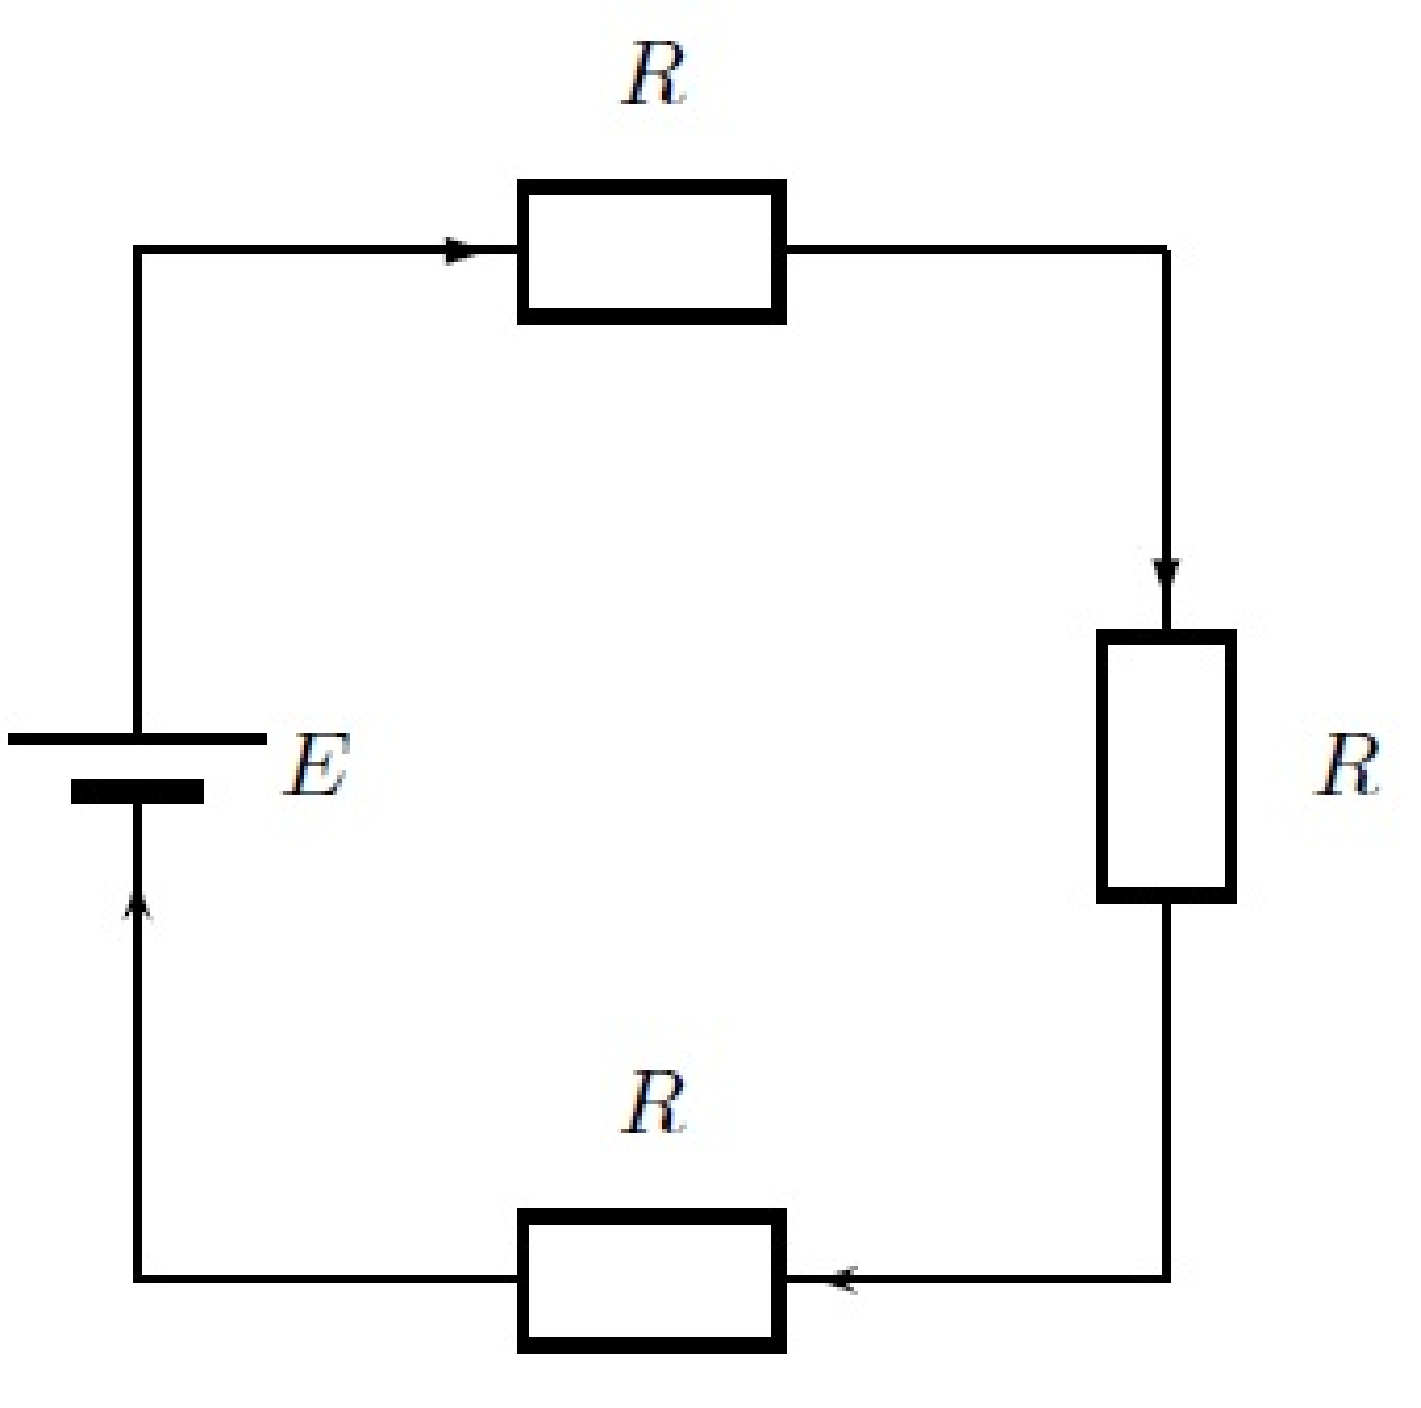
\includegraphics[width=0.4\columnwidth]{col11305.imgs/m38773_PG10C9_026.png} % m38773;PG10C9\_026.png;;;6.0;8.5;
        
      \vspace{2pt}
    \vspace{.1in}
    
    \end{center}

 \end{figure}   

    \addtocounter{footnote}{-0}
    
        \par 

        \label{m38773*id66821}The arrows in this picture show you the direction that charge will flow in the circuit. Note that the arrows point from the positive end of the battery, through the circuit, towards the negative end of the battery. \par 
\label{m38773*notfhsst!!!underscore!!!id1598}
\begin{tabular}{cc}
	\hspace*{-50pt}\raisebox{-8 mm}{\hspace{-0.2in}
\includegraphics[width=0.75in]{col11305.imgs/psfact2.png} } & 

	\begin{minipage}{0.85\textwidth}
	\begin{note}
      {note: }  Benjamin Franklin made a guess about the
direction of charge flow when rubbing smooth wax with rough wool.
He thought that the charges flowed from the wax to the wool (i.e.
from positive to negative) which was opposite to the real
direction. Due to this, electrons are said to have a
\textsl{negative} charge and so objects which Ben Franklin called "negative" (meaning a shortage of charge) really have an excess
of electrons. By the time the true direction of electron flow was
discovered, the convention of ´positive!` and ´negative!` had
already been so well accepted in the scientific world that no
effort was made to change it.
	\end{note}
	\end{minipage}
	\end{tabular}
	\par
      
\label{m38773*notfhsst!!!underscore!!!id1609}
\begin{tabular}{cc}
	   \hspace*{-50pt}\raisebox{-8 mm}{ 
\includegraphics[width=0.5in]{col11305.imgs/pstip2.png}  }& 

	\begin{minipage}{0.85\textwidth}
	\begin{note}
      {tip: }A battery \textbf{does not} produce the same amount of
current no matter what is connected to it. While the voltage
produced by a battery is constant, the amount of current supplied
depends on what is in the circuit.
	\end{note}
	\end{minipage}
	\end{tabular}
	\par
      

    \label{m38773*eip-432}
            \subsubsection{ Exercises: Current}
            \nopagebreak
            
    \par
            \label{m38773*exid001}\vspace{.5cm} 
      
      \noindent
      \hspace*{-30pt}
\includegraphics[width=0.5in]{col11305.imgs/pspencil2.png}   \raisebox{25mm}{   
      \begin{mdframed}[linewidth=4, leftmargin=40, rightmargin=40]  
      \begin{exercise}
    \noindent\textbf{Exercise 16.7}
\label{m38773*prob001}\label{m38773*id001}Using the relationship between current, charge, and time, calculate the current in a circuit which has \begin{math}0,8\phantom{\rule{2pt}{0ex}}\mathrm{C}\end{math} of charge passing a point every second.\par \vspace{5pt}
    \label{m38773*sol001}\noindent\textbf{Solution to Exercise }
\label{m38773*list001}\begin{enumerate}[noitemsep, label=\textbf{Step} \textbf{\arabic*}. ] 
            \leftskip=20pt\rightskip=\leftskip\item 
\begin{math}I=\frac{Q}{\Delta t}\end{math}\label{m38773*id1171063445204}\item 
   \label{m38773*id5231}Given:  \begin{math}Q=0,8\phantom{\rule{2pt}{0ex}}\mathrm{C}\end{math}
    \label{m38773*id1171039489488}\nopagebreak\noindent{}\settowidth{\mymathboxwidth}{\begin{equation}
    \Delta t=1\phantom{\rule{2pt}{0ex}}\mathrm{s}\tag{16.27}
      \end{equation}
    }
    \typeout{Columnwidth = \the\columnwidth}\typeout{math as usual width = \the\mymathboxwidth}
    \ifthenelse{\lengthtest{\mymathboxwidth < \columnwidth}}{% if the math fits, do it again, for real
    \begin{equation}
    \Delta t=1\phantom{\rule{2pt}{0ex}}\mathrm{s}\tag{16.27}
      \end{equation}
    }{% else, if it doesn't fit
    \setlength{\mymathboxwidth}{\columnwidth}
      \addtolength{\mymathboxwidth}{-48pt}
    \par\vspace{12pt}\noindent\begin{minipage}{\columnwidth}
    \parbox[t]{\mymathboxwidth}{\large\begin{math}
    \Delta t=1\phantom{\rule{2pt}{0ex}}\mathrm{s}\end{math}}\hfill
    \parbox[t]{48pt}{\raggedleft 
    (16.27)}
    \end{minipage}\vspace{12pt}\par
    }% end of conditional for this bit of math
    \typeout{math as usual width = \the\mymathboxwidth}
    \par 
    \label{m38773*id1171039728748}Asked for: I\par \label{m38773*id1171061282187}\item 
    \label{m38773*id1171074578672}\nopagebreak\noindent{}\settowidth{\mymathboxwidth}{\begin{equation}
    \begin{array}{ccc}I=\frac{0,8\phantom{\rule{2pt}{0ex}}\mathrm{C}}{1\phantom{\rule{2pt}{0ex}}\mathrm{s}}\\ \phantom{x}=0,8\phantom{\rule{2pt}{0ex}}\mathrm{A}\end{array}\tag{16.28}
      \end{equation}
    }
    \typeout{Columnwidth = \the\columnwidth}\typeout{math as usual width = \the\mymathboxwidth}
    \ifthenelse{\lengthtest{\mymathboxwidth < \columnwidth}}{% if the math fits, do it again, for real
    \begin{equation}
    \begin{array}{ccc}I=\frac{0,8\phantom{\rule{2pt}{0ex}}\mathrm{C}}{1\phantom{\rule{2pt}{0ex}}\mathrm{s}}\\ \phantom{x}=0,8\phantom{\rule{2pt}{0ex}}\mathrm{A}\end{array}\tag{16.28}
      \end{equation}
    }{% else, if it doesn't fit
    \setlength{\mymathboxwidth}{\columnwidth}
      \addtolength{\mymathboxwidth}{-48pt}
    \par\vspace{12pt}\noindent\begin{minipage}{\columnwidth}
    \parbox[t]{\mymathboxwidth}{\large\begin{math}
    I=\frac{0,8\phantom{\rule{2pt}{0ex}}\mathrm{C}}{1\phantom{\rule{2pt}{0ex}}\mathrm{s}}\phantom{x}=0,8\phantom{\rule{2pt}{0ex}}\mathrm{A}\end{math}}\hfill
    \parbox[t]{48pt}{\raggedleft 
    (16.28)}
    \end{minipage}\vspace{12pt}\par
    }% end of conditional for this bit of math
    \typeout{math as usual width = \the\mymathboxwidth}
    \end{enumerate}
        


    \end{exercise}
    \end{mdframed}
    }
    \noindent
  
    
\par
            \label{m38773*exid002}\vspace{.5cm} 
      
      \noindent
      \hspace*{-30pt}
\includegraphics[width=0.5in]{col11305.imgs/pspencil2.png}   \raisebox{25mm}{   
      \begin{mdframed}[linewidth=4, leftmargin=40, rightmargin=40]  
      \begin{exercise}
    \noindent\textbf{Exercise 16.8}
\label{m38773*prob002}
    \label{m38773*id1171059049665}How much charge flows per second in a circuit with a current of \begin{math}1,5\phantom{\rule{2pt}{0ex}}\mathrm{A}\end{math}?\par \vspace{5pt}
\label{m38773*sol002}\noindent\textbf{Solution to Exercise }
\label{m38773*list002}\begin{enumerate}[noitemsep, label=\textbf{Step} \textbf{\arabic*}. ] 
            \leftskip=20pt\rightskip=\leftskip\label{m38773*id1171065905184}\item 
    \label{m38773*id1171057299844}Asked for: Charge, Q\par 
    \label{m38773*id1171060317947}Given: Current \begin{math}I=1,5\phantom{\rule{2pt}{0ex}}\mathrm{A}\end{math}
\label{m38773*id63221}\nopagebreak\noindent{}\settowidth{\mymathboxwidth}{\begin{equation}
    \Delta t=1\phantom{\rule{2pt}{0ex}}\mathrm{s}\tag{16.29}
      \end{equation}
    }
    \typeout{Columnwidth = \the\columnwidth}\typeout{math as usual width = \the\mymathboxwidth}
    \ifthenelse{\lengthtest{\mymathboxwidth < \columnwidth}}{% if the math fits, do it again, for real
    \begin{equation}
    \Delta t=1\phantom{\rule{2pt}{0ex}}\mathrm{s}\tag{16.29}
      \end{equation}
    }{% else, if it doesn't fit
    \setlength{\mymathboxwidth}{\columnwidth}
      \addtolength{\mymathboxwidth}{-48pt}
    \par\vspace{12pt}\noindent\begin{minipage}{\columnwidth}
    \parbox[t]{\mymathboxwidth}{\large\begin{math}
    \Delta t=1\phantom{\rule{2pt}{0ex}}\mathrm{s}\end{math}}\hfill
    \parbox[t]{48pt}{\raggedleft 
    (16.29)}
    \end{minipage}\vspace{12pt}\par
    }% end of conditional for this bit of math
    \typeout{math as usual width = \the\mymathboxwidth}
    \par \label{m38773*id8200544}\item 
    
\begin{math}I=\frac{Q}{\Delta t}\end{math}\label{m38773*id1171079960509}\item 
 \label{m38773*id63232}\begin{math}\begin{array}{ccc}\hfill Q& =& I\ensuremath{\times}\Delta t\hfill \\ & =& \hfill 1,5\phantom{\rule{2pt}{0ex}}\mathrm{A}\ensuremath{\times}1\phantom{\rule{2pt}{0ex}}\mathrm{s}\\ & =& 1,5\phantom{\rule{2pt}{0ex}}\mathrm{C}\hfill \end{array}\end{math}\par \end{enumerate}
        
    \end{exercise}
    \end{mdframed}
    }
    \noindent
  

    
\par
            \label{m38773*exid003}\vspace{.5cm} 
      
      \noindent
      \hspace*{-30pt}
\includegraphics[width=0.5in]{col11305.imgs/pspencil2.png}   \raisebox{25mm}{   
      \begin{mdframed}[linewidth=4, leftmargin=40, rightmargin=40]  
      \begin{exercise}
    \noindent\textbf{Exercise 16.9}\label{m38773*prob003}
    \label{m38773*id1171054423129}If
\begin{math}500\ensuremath{\times}{10}^{3}\phantom{\rule{2pt}{0ex}}\mathrm{\mu C}\end{math} of charge flow past a point in a circuit in 1 second, what is the current in the circuit?\par \vspace{5pt}
\label{m38773*sol003}\noindent\textbf{Solution to Exercise }
\label{m38773*list003}\begin{enumerate}[noitemsep, label=\textbf{Step} \textbf{\arabic*}. ] 
            \leftskip=20pt\rightskip=\leftskip\label{m38773*id1171063940088}\item 
    \label{m38773*id1171053026633}Asked for: current, I\par 
    \label{m38773*id1171039328773}Given: charge
\begin{math}Q=500\ensuremath{\times}{10}^{3}\phantom{\rule{2pt}{0ex}}\mathrm{\mu C}\end{math}\newline
    
\begin{math}\Delta t=1\phantom{\rule{2pt}{0ex}}s\end{math}\par \label{m38773*id1171060421643}\item 
    \label{m38773*id1171064282112}
\begin{math}\begin{array}{ccc}Q=500\ensuremath{\times}{10}^{3}\mathrm{\mu C}\\ \phantom{x}=500\ensuremath{\times}{10}^{3}\ensuremath{\times}{10}^{-6}\mathrm{C}\\ \phantom{x}=0,5\mathrm{C}\end{array}\end{math}\par \label{m38773*id1171073988790}\item 
    \label{m38773*id1171070413749}
\begin{math}I=\frac{Q}{\Delta t}\end{math}\par \label{m38773*id1171058642138}\item 
    \label{m38773*id1171065081814}
\begin{math}\begin{array}{ccc}I=\frac{Q}{\Delta t}\\ \phantom{x}=\frac{0,5\mathrm{C}}{1\mathrm{s}}\\ \phantom{x}=0,5A\end{array}\end{math}\par \end{enumerate}
        
    \end{exercise}
    \end{mdframed}
    }
    \noindent
  
    
\par
            \label{m38773*exid004}\vspace{.5cm} 
      
      \noindent
      \hspace*{-30pt}
\includegraphics[width=0.5in]{col11305.imgs/pspencil2.png}   \raisebox{25mm}{   
      \begin{mdframed}[linewidth=4, leftmargin=40, rightmargin=40]  
      \begin{exercise}
    \noindent\textbf{Exercise 16.10}
\label{m38773*probid004}\label{m38773*id79322}I measure the current in a circuit to be \begin{math}500\mathrm{mA}\end{math}. How much charge is flowing per second in the circuit?\par \vspace{5pt}
\label{m38773*sol004}\noindent\textbf{Solution to Exercise }
\label{m38773*id63422}\begin{enumerate}[noitemsep, label=\textbf{Step} \textbf{\arabic*}. ] 
            \leftskip=20pt\rightskip=\leftskip\label{m38773*id1171076883338}\item 
    \label{m38773*id1171055617645}Asked for: Charge, Q\par 
    \label{m38773*id1171057231899}Given: Current \begin{math}I=500\mathrm{mA}\end{math},\newline
    
\begin{math}\Delta t=1\mathrm{s}\end{math}\par \label{m38773*id1171039664927}\item 
    \label{m38773*id1171056388289}\begin{math}500\mathrm{mA}=500\ensuremath{\times}{10}^{-3}\mathrm{A}\end{math}\par \label{m38773*id1171060384487}\item 
    \label{m38773*id1171065150053}
\begin{math}I=\frac{Q}{\Delta t}\end{math}\par \label{m38773*id1171060172284}\item 
    \label{m38773*id1171039206323}\begin{math}\begin{array}{ccc}Q=I\ensuremath{\times}\Delta t\\ \phantom{x}=500\ensuremath{\times}{10}^{-3}\mathrm{A}\ensuremath{\times}1\mathrm{s}\\ \phantom{x}=0,5\phantom{\rule{2pt}{0ex}}\mathrm{C}\end{array}\end{math}\par \end{enumerate}
        
    \end{exercise}
    \end{mdframed}
    }
    \noindent
  
  

      


    \label{m38773*cid6}
            \subsubsection{ Measuring voltage and current in circuits}
            \nopagebreak
            
      
      \label{m38773*id67616}As we have seen in previous sections, an electric circuit is made
up of a number of different components such as batteries, resistors and
light bulbs. There are devices to measure the properties of these components.
These devices are called meters.\par 
      \label{m38773*id67622}For example, one may be interested in measuring the
amount of current flowing through a circuit using an \textsl{ammeter} or measuring the
voltage provided by a battery using a \textsl{voltmeter}. In this section we will discuss the
practical usage of voltmeters and ammeters.\par 
      \label{m38773*uid72}
            \subsubsection{ Voltmeter}
            \nopagebreak
            
        
        \label{m38773*id67653}A voltmeter is an instrument for measuring the voltage between two
points in an electric circuit. In analogy with a water circuit, a
voltmeter is like a meter designed to measure pressure difference.
Since one is interested in measuring the voltage between two
points in a circuit, a voltmeter must be connected in
\textsl{parallel} with the portion of the circuit on which the
measurement is made.\par 
        
    \setcounter{subfigure}{0}


	\begin{figure}[H] % horizontal\label{m38773*uid73}
    \begin{center}
    \rule[.1in]{\figurerulewidth}{.005in} \\
        \label{m38773*uid73!!!underscore!!!media}\label{m38773*uid73!!!underscore!!!printimage}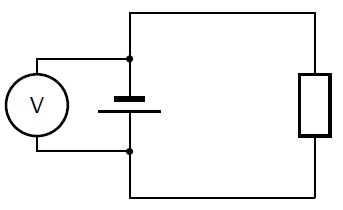
\includegraphics[width=0.4\columnwidth]{col11305.imgs/m38773_PG10C9_034.png} % m38773;PG10C9\_034.png;;;6.0;8.5;
        
      \vspace{2pt}
    \vspace{\rubberspace}\par \begin{cnxcaption}
	  \small \textbf{Figure 16.23: }A voltmeter should be connected in parallel in a circuit.
	\end{cnxcaption}
      
    \vspace{.1in}
    \rule[.1in]{\figurerulewidth}{.005in} \\
        
    \end{center}

 \end{figure}   

    \addtocounter{footnote}{-0}
    
        \label{m38773*id67678}Figure~16.23 shows a voltmeter connected
in parallel with a battery. The positive lead of the voltmeter must be connected closest to the positive end of the battery and the negative lead closest to the negative end of the battery. The voltmeter may also be used to measure the
voltage across a resistor or any other component of a circuit that has a voltage drop or potential difference.\par 
      
      \label{m38773*uid74}
            \subsubsection{ Ammeter}
            \nopagebreak
            
        
        \label{m38773*id62484}An ammeter is an instrument used to measure the flow of electric
current in a circuit. Since one is interested in measuring the
current flowing \textsl{through} the circuit, the ammeter
must be connected in \textsl{series} with the measured circuit
component (Figure~16.24). The positive lead from the ammeter must be connected closest to the positive end of the battery and the negative lead must be connected closest to the negative end of the battery.\par 
        
    \setcounter{subfigure}{0}


	\begin{figure}[H] % horizontal\label{m38773*uid75}
    \begin{center}
    \rule[.1in]{\figurerulewidth}{.005in} \\
        \label{m38773*uid75!!!underscore!!!media}\label{m38773*uid75!!!underscore!!!printimage}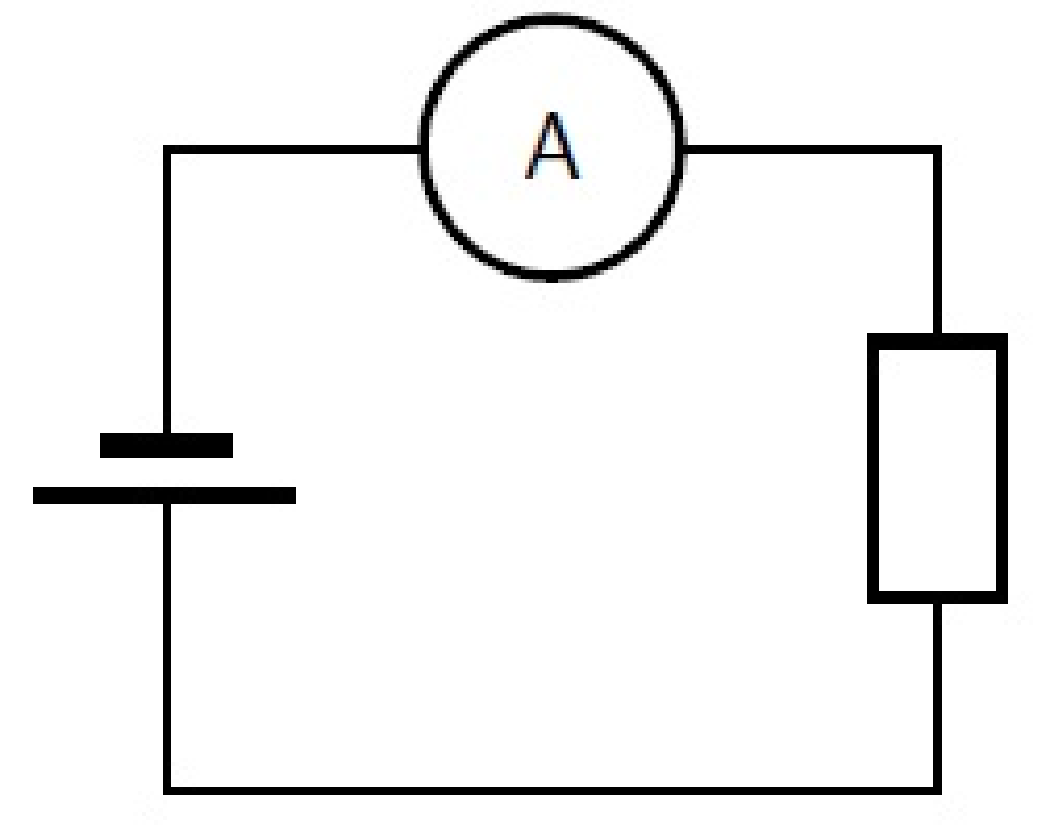
\includegraphics[width=0.4\columnwidth]{col11305.imgs/m38773_PG10C9_035.png} % m38773;PG10C9\_035.png;;;6.0;8.5;
        
      \vspace{2pt}
    \vspace{\rubberspace}\par \begin{cnxcaption}
	  \small \textbf{Figure 16.24: }An ammeter should be connected in series in a circuit.
	\end{cnxcaption}
      
    \vspace{.1in}
    \rule[.1in]{\figurerulewidth}{.005in} \\
        
    \end{center}

 \end{figure}   

    \addtocounter{footnote}{-0}
    
      

 

      \label{m38773*uid78}
            \subsubsection{ Impact of meters on circuits}
            \nopagebreak
            
        
        \label{m38773*id67854}A good quality meter used correctly will not significantly change
the values it is used to measure. This means that an ammeter has
very low resistance so as to not slow down the flow of charge. A voltmeter has a very high resistance so that it does not add another
parallel pathway to the circuit for the charge to flow along.\par 
\label{m38773*secfhsst!!!underscore!!!id1891}
            \subsubsection{  Investigation : Using meters }
            \nopagebreak
            
        \label{m38773*id67868}If possible,
connect meters in circuits to get used to how to use meters to
measure electrical quantities. If the meters have more than one
scale, always connect to the \textbf{largest scale} first so that the meter
will not be damaged by having to measure values that exceed its
limits. \par 

        \label{m38773*id67887}The table below summarises the use of each measuring instrument
that we discussed and the way it should be connected to a circuit
component.\par 
        
    % \textbf{m38773*id67892}\par
    
    % how many colspecs?  3
          % name: cnx:colspec
            % colnum: 1
            % colwidth: 10*
            % latex-name: columna
            % colname: 
            % align/tgroup-align/default: //left
            % -------------------------
            % name: cnx:colspec
            % colnum: 2
            % colwidth: 10*
            % latex-name: columnb
            % colname: 
            % align/tgroup-align/default: //left
            % -------------------------
            % name: cnx:colspec
            % colnum: 3
            % colwidth: 10*
            % latex-name: columnc
            % colname: 
            % align/tgroup-align/default: //left
            % -------------------------
      
    
    \setlength\mytablespace{6\tabcolsep}
    \addtolength\mytablespace{4\arrayrulewidth}
    \setlength\mytablewidth{\linewidth}
        
    
    \setlength\mytableroom{\mytablewidth}
    \addtolength\mytableroom{-\mytablespace}
    
    \setlength\myfixedwidth{0pt}
    \setlength\mystarwidth{\mytableroom}
        \addtolength\mystarwidth{-\myfixedwidth}
        \divide\mystarwidth 30
        
    
      % ----- Begin capturing width of table in LR mode woof
      \settowidth{\mytableboxwidth}{\begin{tabular}[t]{|l|l|l|}\hline
    % count in rowspan-info-nodeset: 3
    % align/colidx: left,1
    
    % rowcount: '0' | start: 'false' | colidx: '1'
    
        % Formatting a regular cell and recurring on the next sibling
        
                  \textbf{Instrument}
                 &
      % align/colidx: left,2
    
    % rowcount: '0' | start: 'false' | colidx: '2'
    
        % Formatting a regular cell and recurring on the next sibling
        
                  \textbf{Measured Quantity}
                 &
      % align/colidx: left,3
    
    % rowcount: '0' | start: 'false' | colidx: '3'
    
        % Formatting a regular cell and recurring on the next sibling
        
                  \textbf{Proper Connection}
                % make-rowspan-placeholders
    % rowspan info: col1 '0' | 'false' | '' || col2 '0' | 'false' | '' || col3 '0' | 'false' | ''
     \tabularnewline\cline{1-1}\cline{2-2}\cline{3-3}
      %--------------------------------------------------------------------
    % align/colidx: left,1
    
    % rowcount: '0' | start: 'false' | colidx: '1'
    
        % Formatting a regular cell and recurring on the next sibling
        Voltmeter &
      % align/colidx: left,2
    
    % rowcount: '0' | start: 'false' | colidx: '2'
    
        % Formatting a regular cell and recurring on the next sibling
        Voltage &
      % align/colidx: left,3
    
    % rowcount: '0' | start: 'false' | colidx: '3'
    
        % Formatting a regular cell and recurring on the next sibling
        In Parallel% make-rowspan-placeholders
    % rowspan info: col1 '0' | 'false' | '' || col2 '0' | 'false' | '' || col3 '0' | 'false' | ''
     \tabularnewline\cline{1-1}\cline{2-2}\cline{3-3}
      %--------------------------------------------------------------------
    % align/colidx: left,1
    
    % rowcount: '0' | start: 'false' | colidx: '1'
    
        % Formatting a regular cell and recurring on the next sibling
        Ammeter &
      % align/colidx: left,2
    
    % rowcount: '0' | start: 'false' | colidx: '2'
    
        % Formatting a regular cell and recurring on the next sibling
        Current &
      % align/colidx: left,3
    
    % rowcount: '0' | start: 'false' | colidx: '3'
    
        % Formatting a regular cell and recurring on the next sibling
        In Series% make-rowspan-placeholders
    % rowspan info: col1 '0' | 'false' | '' || col2 '0' | 'false' | '' || col3 '0' | 'false' | ''
     \tabularnewline\cline{1-1}\cline{2-2}\cline{3-3}
      %--------------------------------------------------------------------
    \end{tabular}} % end mytableboxwidth set
      \addtocounter{footnote}{-0}
      
      % ----- End capturing width of table in LR mode
    
        % ----- LR or paragraph mode: must test
        % ----- Begin capturing height of table
        \settoheight{\mytableboxheight}{\begin{tabular}[t]{|l|l|l|}\hline
    % count in rowspan-info-nodeset: 3
    % align/colidx: left,1
    
    % rowcount: '0' | start: 'false' | colidx: '1'
    
        % Formatting a regular cell and recurring on the next sibling
        
                  \textbf{Instrument}
                 &
      % align/colidx: left,2
    
    % rowcount: '0' | start: 'false' | colidx: '2'
    
        % Formatting a regular cell and recurring on the next sibling
        
                  \textbf{Measured Quantity}
                 &
      % align/colidx: left,3
    
    % rowcount: '0' | start: 'false' | colidx: '3'
    
        % Formatting a regular cell and recurring on the next sibling
        
                  \textbf{Proper Connection}
                % make-rowspan-placeholders
    % rowspan info: col1 '0' | 'false' | '' || col2 '0' | 'false' | '' || col3 '0' | 'false' | ''
     \tabularnewline\cline{1-1}\cline{2-2}\cline{3-3}
      %--------------------------------------------------------------------
    % align/colidx: left,1
    
    % rowcount: '0' | start: 'false' | colidx: '1'
    
        % Formatting a regular cell and recurring on the next sibling
        Voltmeter &
      % align/colidx: left,2
    
    % rowcount: '0' | start: 'false' | colidx: '2'
    
        % Formatting a regular cell and recurring on the next sibling
        Voltage &
      % align/colidx: left,3
    
    % rowcount: '0' | start: 'false' | colidx: '3'
    
        % Formatting a regular cell and recurring on the next sibling
        In Parallel% make-rowspan-placeholders
    % rowspan info: col1 '0' | 'false' | '' || col2 '0' | 'false' | '' || col3 '0' | 'false' | ''
     \tabularnewline\cline{1-1}\cline{2-2}\cline{3-3}
      %--------------------------------------------------------------------
    % align/colidx: left,1
    
    % rowcount: '0' | start: 'false' | colidx: '1'
    
        % Formatting a regular cell and recurring on the next sibling
        Ammeter &
      % align/colidx: left,2
    
    % rowcount: '0' | start: 'false' | colidx: '2'
    
        % Formatting a regular cell and recurring on the next sibling
        Current &
      % align/colidx: left,3
    
    % rowcount: '0' | start: 'false' | colidx: '3'
    
        % Formatting a regular cell and recurring on the next sibling
        In Series% make-rowspan-placeholders
    % rowspan info: col1 '0' | 'false' | '' || col2 '0' | 'false' | '' || col3 '0' | 'false' | ''
     \tabularnewline\cline{1-1}\cline{2-2}\cline{3-3}
      %--------------------------------------------------------------------
    \end{tabular}} % end mytableboxheight set
        \settodepth{\mytableboxdepth}{\begin{tabular}[t]{|l|l|l|}\hline
    % count in rowspan-info-nodeset: 3
    % align/colidx: left,1
    
    % rowcount: '0' | start: 'false' | colidx: '1'
    
        % Formatting a regular cell and recurring on the next sibling
        
                  \textbf{Instrument}
                 &
      % align/colidx: left,2
    
    % rowcount: '0' | start: 'false' | colidx: '2'
    
        % Formatting a regular cell and recurring on the next sibling
        
                  \textbf{Measured Quantity}
                 &
      % align/colidx: left,3
    
    % rowcount: '0' | start: 'false' | colidx: '3'
    
        % Formatting a regular cell and recurring on the next sibling
        
                  \textbf{Proper Connection}
                % make-rowspan-placeholders
    % rowspan info: col1 '0' | 'false' | '' || col2 '0' | 'false' | '' || col3 '0' | 'false' | ''
     \tabularnewline\cline{1-1}\cline{2-2}\cline{3-3}
      %--------------------------------------------------------------------
    % align/colidx: left,1
    
    % rowcount: '0' | start: 'false' | colidx: '1'
    
        % Formatting a regular cell and recurring on the next sibling
        Voltmeter &
      % align/colidx: left,2
    
    % rowcount: '0' | start: 'false' | colidx: '2'
    
        % Formatting a regular cell and recurring on the next sibling
        Voltage &
      % align/colidx: left,3
    
    % rowcount: '0' | start: 'false' | colidx: '3'
    
        % Formatting a regular cell and recurring on the next sibling
        In Parallel% make-rowspan-placeholders
    % rowspan info: col1 '0' | 'false' | '' || col2 '0' | 'false' | '' || col3 '0' | 'false' | ''
     \tabularnewline\cline{1-1}\cline{2-2}\cline{3-3}
      %--------------------------------------------------------------------
    % align/colidx: left,1
    
    % rowcount: '0' | start: 'false' | colidx: '1'
    
        % Formatting a regular cell and recurring on the next sibling
        Ammeter &
      % align/colidx: left,2
    
    % rowcount: '0' | start: 'false' | colidx: '2'
    
        % Formatting a regular cell and recurring on the next sibling
        Current &
      % align/colidx: left,3
    
    % rowcount: '0' | start: 'false' | colidx: '3'
    
        % Formatting a regular cell and recurring on the next sibling
        In Series% make-rowspan-placeholders
    % rowspan info: col1 '0' | 'false' | '' || col2 '0' | 'false' | '' || col3 '0' | 'false' | ''
     \tabularnewline\cline{1-1}\cline{2-2}\cline{3-3}
      %--------------------------------------------------------------------
    \end{tabular}} % end mytableboxdepth set
        \addtolength{\mytableboxheight}{\mytableboxdepth}
        % ----- End capturing height of table
        \addtocounter{footnote}{-0}
        
        \ifthenelse{\mytableboxwidth<\textwidth}{% the table fits in LR mode
          \addtolength{\mytableboxwidth}{-\mytablespace}
          \typeout{textheight: \the\textheight}
          \typeout{mytableboxheight: \the\mytableboxheight}
          \typeout{textwidth: \the\textwidth}
          \typeout{mytableboxwidth: \the\mytableboxwidth}
          \ifthenelse{\mytableboxheight<\textheight}{%
        
    % \begin{table}[H]
    % \\ '' '0'
    
        \begin{center}
      
      \label{m38773*id67892}
      
    \noindent
    \begin{tabular}[t]{|l|l|l|}\hline
    % count in rowspan-info-nodeset: 3
    % align/colidx: left,1
    
    % rowcount: '0' | start: 'false' | colidx: '1'
    
        % Formatting a regular cell and recurring on the next sibling
        
                  \textbf{Instrument}
                 &
      % align/colidx: left,2
    
    % rowcount: '0' | start: 'false' | colidx: '2'
    
        % Formatting a regular cell and recurring on the next sibling
        
                  \textbf{Measured Quantity}
                 &
      % align/colidx: left,3
    
    % rowcount: '0' | start: 'false' | colidx: '3'
    
        % Formatting a regular cell and recurring on the next sibling
        
                  \textbf{Proper Connection}
                % make-rowspan-placeholders
    % rowspan info: col1 '0' | 'false' | '' || col2 '0' | 'false' | '' || col3 '0' | 'false' | ''
     \tabularnewline\cline{1-1}\cline{2-2}\cline{3-3}
      %--------------------------------------------------------------------
    % align/colidx: left,1
    
    % rowcount: '0' | start: 'false' | colidx: '1'
    
        % Formatting a regular cell and recurring on the next sibling
        Voltmeter &
      % align/colidx: left,2
    
    % rowcount: '0' | start: 'false' | colidx: '2'
    
        % Formatting a regular cell and recurring on the next sibling
        Voltage &
      % align/colidx: left,3
    
    % rowcount: '0' | start: 'false' | colidx: '3'
    
        % Formatting a regular cell and recurring on the next sibling
        In Parallel% make-rowspan-placeholders
    % rowspan info: col1 '0' | 'false' | '' || col2 '0' | 'false' | '' || col3 '0' | 'false' | ''
     \tabularnewline\cline{1-1}\cline{2-2}\cline{3-3}
      %--------------------------------------------------------------------
    % align/colidx: left,1
    
    % rowcount: '0' | start: 'false' | colidx: '1'
    
        % Formatting a regular cell and recurring on the next sibling
        Ammeter &
      % align/colidx: left,2
    
    % rowcount: '0' | start: 'false' | colidx: '2'
    
        % Formatting a regular cell and recurring on the next sibling
        Current &
      % align/colidx: left,3
    
    % rowcount: '0' | start: 'false' | colidx: '3'
    
        % Formatting a regular cell and recurring on the next sibling
        In Series% make-rowspan-placeholders
    % rowspan info: col1 '0' | 'false' | '' || col2 '0' | 'false' | '' || col3 '0' | 'false' | ''
     \tabularnewline\cline{1-1}\cline{2-2}\cline{3-3}
      %--------------------------------------------------------------------
    \end{tabular}
      \end{center}
    \begin{center}{\small\bfseries Table 16.2}\end{center}
    %\end{table}
    
    \addtocounter{footnote}{-0}
    
          }{ % else
        
    % \begin{table}[H]
    % \\ '' '0'
    
        \begin{center}
      
      \label{m38773*id67892}
      
    \noindent
    \tabletail{%
        \hline
        \multicolumn{3}{|p{\mytableboxwidth}|}{\raggedleft \small \sl continued on next page}\\
        \hline
      }
      \tablelasttail{}
      \begin{xtabular}[t]{|l|l|l|}\hline
    % count in rowspan-info-nodeset: 3
    % align/colidx: left,1
    
    % rowcount: '0' | start: 'false' | colidx: '1'
    
        % Formatting a regular cell and recurring on the next sibling
        
                  \textbf{Instrument}
                 &
      % align/colidx: left,2
    
    % rowcount: '0' | start: 'false' | colidx: '2'
    
        % Formatting a regular cell and recurring on the next sibling
        
                  \textbf{Measured Quantity}
                 &
      % align/colidx: left,3
    
    % rowcount: '0' | start: 'false' | colidx: '3'
    
        % Formatting a regular cell and recurring on the next sibling
        
                  \textbf{Proper Connection}
                % make-rowspan-placeholders
    % rowspan info: col1 '0' | 'false' | '' || col2 '0' | 'false' | '' || col3 '0' | 'false' | ''
     \tabularnewline\cline{1-1}\cline{2-2}\cline{3-3}
      %--------------------------------------------------------------------
    % align/colidx: left,1
    
    % rowcount: '0' | start: 'false' | colidx: '1'
    
        % Formatting a regular cell and recurring on the next sibling
        Voltmeter &
      % align/colidx: left,2
    
    % rowcount: '0' | start: 'false' | colidx: '2'
    
        % Formatting a regular cell and recurring on the next sibling
        Voltage &
      % align/colidx: left,3
    
    % rowcount: '0' | start: 'false' | colidx: '3'
    
        % Formatting a regular cell and recurring on the next sibling
        In Parallel% make-rowspan-placeholders
    % rowspan info: col1 '0' | 'false' | '' || col2 '0' | 'false' | '' || col3 '0' | 'false' | ''
     \tabularnewline\cline{1-1}\cline{2-2}\cline{3-3}
      %--------------------------------------------------------------------
    % align/colidx: left,1
    
    % rowcount: '0' | start: 'false' | colidx: '1'
    
        % Formatting a regular cell and recurring on the next sibling
        Ammeter &
      % align/colidx: left,2
    
    % rowcount: '0' | start: 'false' | colidx: '2'
    
        % Formatting a regular cell and recurring on the next sibling
        Current &
      % align/colidx: left,3
    
    % rowcount: '0' | start: 'false' | colidx: '3'
    
        % Formatting a regular cell and recurring on the next sibling
        In Series% make-rowspan-placeholders
    % rowspan info: col1 '0' | 'false' | '' || col2 '0' | 'false' | '' || col3 '0' | 'false' | ''
     \tabularnewline\cline{1-1}\cline{2-2}\cline{3-3}
      %--------------------------------------------------------------------
    \end{xtabular}
      \end{center}
    \begin{center}{\small\bfseries Table 16.2}\end{center}
    %\end{table}
    
    \addtocounter{footnote}{-0}
    
          } % 
        }{% else
        % typeset the table in paragraph mode
        % ----- Begin capturing height of table
        \settoheight{\mytableboxheight}{\begin{tabular*}{\mytablewidth}[t]{|p{10\mystarwidth}|p{10\mystarwidth}|p{10\mystarwidth}|}\hline
    % count in rowspan-info-nodeset: 3
    % align/colidx: left,1
    
    % rowcount: '0' | start: 'false' | colidx: '1'
    
        % Formatting a regular cell and recurring on the next sibling
        
                  \textbf{Instrument}
                 &
      % align/colidx: left,2
    
    % rowcount: '0' | start: 'false' | colidx: '2'
    
        % Formatting a regular cell and recurring on the next sibling
        
                  \textbf{Measured Quantity}
                 &
      % align/colidx: left,3
    
    % rowcount: '0' | start: 'false' | colidx: '3'
    
        % Formatting a regular cell and recurring on the next sibling
        
                  \textbf{Proper Connection}
                % make-rowspan-placeholders
    % rowspan info: col1 '0' | 'false' | '' || col2 '0' | 'false' | '' || col3 '0' | 'false' | ''
     \tabularnewline\cline{1-1}\cline{2-2}\cline{3-3}
      %--------------------------------------------------------------------
    % align/colidx: left,1
    
    % rowcount: '0' | start: 'false' | colidx: '1'
    
        % Formatting a regular cell and recurring on the next sibling
        Voltmeter &
      % align/colidx: left,2
    
    % rowcount: '0' | start: 'false' | colidx: '2'
    
        % Formatting a regular cell and recurring on the next sibling
        Voltage &
      % align/colidx: left,3
    
    % rowcount: '0' | start: 'false' | colidx: '3'
    
        % Formatting a regular cell and recurring on the next sibling
        In Parallel% make-rowspan-placeholders
    % rowspan info: col1 '0' | 'false' | '' || col2 '0' | 'false' | '' || col3 '0' | 'false' | ''
     \tabularnewline\cline{1-1}\cline{2-2}\cline{3-3}
      %--------------------------------------------------------------------
    % align/colidx: left,1
    
    % rowcount: '0' | start: 'false' | colidx: '1'
    
        % Formatting a regular cell and recurring on the next sibling
        Ammeter &
      % align/colidx: left,2
    
    % rowcount: '0' | start: 'false' | colidx: '2'
    
        % Formatting a regular cell and recurring on the next sibling
        Current &
      % align/colidx: left,3
    
    % rowcount: '0' | start: 'false' | colidx: '3'
    
        % Formatting a regular cell and recurring on the next sibling
        In Series% make-rowspan-placeholders
    % rowspan info: col1 '0' | 'false' | '' || col2 '0' | 'false' | '' || col3 '0' | 'false' | ''
     \tabularnewline\cline{1-1}\cline{2-2}\cline{3-3}
      %--------------------------------------------------------------------
    \end{tabular*}} % end mytableboxheight set
        \settodepth{\mytableboxdepth}{\begin{tabular*}{\mytablewidth}[t]{|p{10\mystarwidth}|p{10\mystarwidth}|p{10\mystarwidth}|}\hline
    % count in rowspan-info-nodeset: 3
    % align/colidx: left,1
    
    % rowcount: '0' | start: 'false' | colidx: '1'
    
        % Formatting a regular cell and recurring on the next sibling
        
                  \textbf{Instrument}
                 &
      % align/colidx: left,2
    
    % rowcount: '0' | start: 'false' | colidx: '2'
    
        % Formatting a regular cell and recurring on the next sibling
        
                  \textbf{Measured Quantity}
                 &
      % align/colidx: left,3
    
    % rowcount: '0' | start: 'false' | colidx: '3'
    
        % Formatting a regular cell and recurring on the next sibling
        
                  \textbf{Proper Connection}
                % make-rowspan-placeholders
    % rowspan info: col1 '0' | 'false' | '' || col2 '0' | 'false' | '' || col3 '0' | 'false' | ''
     \tabularnewline\cline{1-1}\cline{2-2}\cline{3-3}
      %--------------------------------------------------------------------
    % align/colidx: left,1
    
    % rowcount: '0' | start: 'false' | colidx: '1'
    
        % Formatting a regular cell and recurring on the next sibling
        Voltmeter &
      % align/colidx: left,2
    
    % rowcount: '0' | start: 'false' | colidx: '2'
    
        % Formatting a regular cell and recurring on the next sibling
        Voltage &
      % align/colidx: left,3
    
    % rowcount: '0' | start: 'false' | colidx: '3'
    
        % Formatting a regular cell and recurring on the next sibling
        In Parallel% make-rowspan-placeholders
    % rowspan info: col1 '0' | 'false' | '' || col2 '0' | 'false' | '' || col3 '0' | 'false' | ''
     \tabularnewline\cline{1-1}\cline{2-2}\cline{3-3}
      %--------------------------------------------------------------------
    % align/colidx: left,1
    
    % rowcount: '0' | start: 'false' | colidx: '1'
    
        % Formatting a regular cell and recurring on the next sibling
        Ammeter &
      % align/colidx: left,2
    
    % rowcount: '0' | start: 'false' | colidx: '2'
    
        % Formatting a regular cell and recurring on the next sibling
        Current &
      % align/colidx: left,3
    
    % rowcount: '0' | start: 'false' | colidx: '3'
    
        % Formatting a regular cell and recurring on the next sibling
        In Series% make-rowspan-placeholders
    % rowspan info: col1 '0' | 'false' | '' || col2 '0' | 'false' | '' || col3 '0' | 'false' | ''
     \tabularnewline\cline{1-1}\cline{2-2}\cline{3-3}
      %--------------------------------------------------------------------
    \end{tabular*}} % end mytableboxdepth set
        \addtolength{\mytableboxheight}{\mytableboxdepth}
        % ----- End capturing height of table
        \typeout{textheight: \the\textheight}
        \typeout{mytableboxheight: \the\mytableboxheight}
        \typeout{table too wide, outputting in para mode}
        
    % \begin{table}[H]
    % \\ '' '0'
    
        \begin{center}
      
      \label{m38773*id67892}
      
    \noindent
    \tabletail{%
        \hline
        \multicolumn{3}{|p{\mytableroom}|}{\raggedleft \small \sl continued on next page}\\
        \hline
      }
      \tablelasttail{}
      \begin{xtabular*}{\mytablewidth}[t]{|p{10\mystarwidth}|p{10\mystarwidth}|p{10\mystarwidth}|}\hline
    % count in rowspan-info-nodeset: 3
    % align/colidx: left,1
    
    % rowcount: '0' | start: 'false' | colidx: '1'
    
        % Formatting a regular cell and recurring on the next sibling
        
                  \textbf{Instrument}
                 &
      % align/colidx: left,2
    
    % rowcount: '0' | start: 'false' | colidx: '2'
    
        % Formatting a regular cell and recurring on the next sibling
        
                  \textbf{Measured Quantity}
                 &
      % align/colidx: left,3
    
    % rowcount: '0' | start: 'false' | colidx: '3'
    
        % Formatting a regular cell and recurring on the next sibling
        
                  \textbf{Proper Connection}
                % make-rowspan-placeholders
    % rowspan info: col1 '0' | 'false' | '' || col2 '0' | 'false' | '' || col3 '0' | 'false' | ''
     \tabularnewline\cline{1-1}\cline{2-2}\cline{3-3}
      %--------------------------------------------------------------------
    % align/colidx: left,1
    
    % rowcount: '0' | start: 'false' | colidx: '1'
    
        % Formatting a regular cell and recurring on the next sibling
        Voltmeter &
      % align/colidx: left,2
    
    % rowcount: '0' | start: 'false' | colidx: '2'
    
        % Formatting a regular cell and recurring on the next sibling
        Voltage &
      % align/colidx: left,3
    
    % rowcount: '0' | start: 'false' | colidx: '3'
    
        % Formatting a regular cell and recurring on the next sibling
        In Parallel% make-rowspan-placeholders
    % rowspan info: col1 '0' | 'false' | '' || col2 '0' | 'false' | '' || col3 '0' | 'false' | ''
     \tabularnewline\cline{1-1}\cline{2-2}\cline{3-3}
      %--------------------------------------------------------------------
    % align/colidx: left,1
    
    % rowcount: '0' | start: 'false' | colidx: '1'
    
        % Formatting a regular cell and recurring on the next sibling
        Ammeter &
      % align/colidx: left,2
    
    % rowcount: '0' | start: 'false' | colidx: '2'
    
        % Formatting a regular cell and recurring on the next sibling
        Current &
      % align/colidx: left,3
    
    % rowcount: '0' | start: 'false' | colidx: '3'
    
        % Formatting a regular cell and recurring on the next sibling
        In Series% make-rowspan-placeholders
    % rowspan info: col1 '0' | 'false' | '' || col2 '0' | 'false' | '' || col3 '0' | 'false' | ''
     \tabularnewline\cline{1-1}\cline{2-2}\cline{3-3}
      %--------------------------------------------------------------------
    \end{xtabular*}
      \end{center}
    \begin{center}{\small\bfseries Table 16.2}\end{center}
    %\end{table}
    
    \addtocounter{footnote}{-0}
    
        }% ending lr/para test clause
      
    \par
  
        
      
     



 

    

  \label{m38773**end}
          
         \section{ Resistance}
    \nopagebreak
            \label{m38776} $ \hspace{-5pt}\begin{array}{cccccccccccc}   
\includegraphics[width=0.75cm]{col11305.imgs/summary_fullmarks.png} &   \includegraphics[width=0.75cm]{col11305.imgs/summary_video.png} &   \end{array} $ \hspace{2 pt}\raisebox{-5 pt}{} {(section shortcode: P10077 )} \par 
    
    
    
    
    
    
  
    \label{m38776*cid5}
            \subsection{ Resistance}
            \nopagebreak
            
      
      \label{m38776*sb1235}
	The resistance of a circuit element can be thought of as how much it opposes the flow of electric current in the circuit. 
	\vspace{\rubberspace}\par
        \label{m38776*fhsst!!!underscore!!!id1729}\begin{definition}
	  \begin{tabular*}{15 cm}{m{15 mm}m{}}
	\hspace*{-50pt}  \includegraphics[width=0.5in]{col11305.imgs/psflag2.png}   & \Definition{   \label{id2485077}\textbf{ Resistance }} { \label{m38776*meaningfhsst!!!underscore!!!id1729}
        \label{m38776*id67260} The resistance of a conductor is defined as the potential difference across it divided by the current flowing though it. We use the symbol \textbf{R} to show resistance and it is measured in units called \textbf{Ohms} with the symbol \begin{math}\mathrm{\Omega }\end{math}.\par 
        \label{m38776*id67288}\nopagebreak\noindent{}
          \settowidth{\mymathboxwidth}{\begin{equation}
    1\phantom{\rule{4pt}{0ex}}\mathrm{Ohm}=1\frac{\mathrm{Volt}}{\mathrm{Ampere}}.\tag{16.30}
      \end{equation}
    }
    \typeout{Columnwidth = \the\columnwidth}\typeout{math as usual width = \the\mymathboxwidth}
    \ifthenelse{\lengthtest{\mymathboxwidth < \columnwidth}}{% if the math fits, do it again, for real
    \begin{equation}
    1\phantom{\rule{4pt}{0ex}}\mathrm{Ohm}=1\frac{\mathrm{Volt}}{\mathrm{Ampere}}.\tag{16.30}
      \end{equation}
    }{% else, if it doesn't fit
    \setlength{\mymathboxwidth}{\columnwidth}
      \addtolength{\mymathboxwidth}{-48pt}
    \par\vspace{12pt}\noindent\begin{minipage}{\columnwidth}
    \parbox[t]{\mymathboxwidth}{\large\begin{math}
    1\phantom{\rule{4pt}{0ex}}\mathrm{Ohm}=1\frac{\mathrm{Volt}}{\mathrm{Ampere}}.\end{math}}\hfill
    \parbox[t]{48pt}{\raggedleft 
    (16.30)}
    \end{minipage}\vspace{12pt}\par
    }% end of conditional for this bit of math
    \typeout{math as usual width = \the\mymathboxwidth}
    
        
        
         } 
      \end{tabular*}
      \end{definition}


	\par 


      \label{m38776*uid62}
            \subsubsection{ What causes resistance?}
            \nopagebreak
            
        
        \label{m38776*id67246}We have spoken about resistors that reduce the flow of charge
in a conductor. On a microscopic level, electrons moving through
the conductor collide with the particles of which the conductor
(metal) is made. When they collide, they transfer kinetic energy.
The electrons lose kinetic energy and slow down. This leads to
resistance. The transferred energy causes the resistor to heat up.
You can feel this directly if you touch a cellphone charger when you are charging a cell phone - the charger gets warm because its circuits have some resistors in them!\par 

        \label{m38776*id67330}\textsl{All} conductors have some resistance. For example, a piece of wire
has less resistance than a light bulb, but both have resistance. A lightbulb is a very thin wire surrounded by a glass housing The high resistance of the filament (small wire) in a lightbulb causes the electrons to
transfer a lot of their kinetic energy in the form of heat\label{m38776*uid63}\footnote{Flourescent lightbulbs do not use thin wires; they use the fact that certain gases glow when a current flows through them. They are much more efficient (much less resistance) than lightbulbs.}. The heat energy is enough
to cause the filament to glow white-hot which produces light. The wires
connecting the lamp to the cell or battery hardly even get warm while
conducting the same amount of current. This is because of their
much lower resistance due to their larger cross-section (they are thicker).\par 
        \label{m38776*id67354}An important effect of a resistor is that it \textsl{converts} electrical
energy into \textbf{heat} energy. \textbf{Light} is a by-product of the heat that is produced.\par 
\label{m38776*notfhsst!!!underscore!!!id1758}
\begin{tabular}{cc}
	\hspace*{-50pt}\raisebox{-8 mm}{\hspace{-0.2in}\includegraphics[width=0.75in]{col11305.imgs/psfact2.png} } & 

	\begin{minipage}{0.85\textwidth}
	\begin{note}
      {note: } There is a special type of conductor,
called a \textbf{superconductor} that has no resistance, but the
materials that make up all known superconductors only start superconducting
at very low temperatures (approximately -170\begin{math}{}^{\circ }\end{math}C).
	\end{note}
	\end{minipage}
	\end{tabular}
	\par
      
       
 \label{m38776*uid64}
            \subsubsection{ Why do batteries go flat?}
            \nopagebreak
            
          
          \label{m38776*id67413}A battery stores chemical potential energy. When it is connected in a circuit, a chemical reaction takes place inside the battery which converts chemical potential energy to electrical energy which powers the charges (electrons) to move through the circuit. All the circuit elements (such as the conducting leads, resistors and lightbulbs) have some resistance to the flow of charge and convert the electrical energy to heat and, in the case of the lightbulb, heat and light.
Since energy is always conserved, the battery goes flat when all its chemical potential energy has been converted into other forms of energy.\par 
        

      
      \label{m38776*uid65}
            \subsubsection{ Resistors in electric circuits}
            \nopagebreak
            
        
        \label{m38776*id67431}It is important to understand what effect adding resistors to a circuit has on the \textsl{total} resistance of a circuit and on the current that can flow in the circuit.\par 
        \label{m38776*uid66}
            \subsubsection{ Resistors in series}
            \nopagebreak
            
          
          \label{m38776*id67450}When we add resistors in series to a circuit, we \textsl{increase} the resistance to the flow of current. There is only \textbf{one path} along which the current can flow and the current is the same at all places in the series circuit. Take a look at the diagram below: On the left there is a circuit with a single resistor and a battery. No matter where we measure the current, it is the same in a series circuit. On the right, we have added a second resistor in series to the circuit. The \textsl{total} resistance of the circuit has \textsl{increased} and you can see from the reading on the ammeter that the current in the circuit has \textsl{decreased} and is still the same everywhere in the circuit.\par 
          \label{m38776*id67481}
            
    \setcounter{subfigure}{0}


	\begin{figure}[H] % horizontal\label{m38776*id67485}
    \begin{center}
    \label{m38776*id67485!!!underscore!!!media}\label{m38776*id67485!!!underscore!!!printimage}\includegraphics{col11305.imgs/m38776_PG10C9_032.png} % m38776;PG10C9\_032.png;;;6.0;8.5;
        
      \vspace{2pt}
    \vspace{.1in}
    
    \end{center}

 \end{figure}   

    \addtocounter{footnote}{-0}
    
          \par 


\label{m38776*id64070}\noindent{}\textbf{Potential difference and resistors in series}When resistors are in series, one after the other, there is a potential difference across each resistor. The total potential difference across a set of resistors in series is the sum of the potential differences across each of the resistors in the set. This is the same as falling a large distance under gravity or falling that same distance (difference) in many smaller steps. The total distance (difference) is the same.\par 
        \label{m38776*id64076}Look at the circuits below. If we measured the potential difference between the black dots in all of these circuits it would be the same; it is just the potential difference across the battery which is the same as the potential difference across the rest of the circuit. So we now know the total potential difference is the same across one, two or three resistors. We also know that some work is required to make charge flow through each one. Each is a step down in potential energy. These steps add up to the total voltage drop which we know is the difference between the two dots.

The sum of the potential differences across each individual resistor is equal to the potential difference measured across all of them together. For this reason, series circuits are sometimes called \textbf{voltage dividers}.\par 
        \label{m38776*id64084}
          
    \setcounter{subfigure}{0}


	\begin{figure}[H] % horizontal\label{m38776*id64087}
    \begin{center}
    \label{m38776*id64087!!!underscore!!!media}\label{m38776*id64087!!!underscore!!!printimage}\includegraphics[width=\columnwidth]{col11305.imgs/m38776_PG10C9_018.png} % m38776;PG10C9\_018.png;;;6.0;8.5;
        
      \vspace{2pt}
    \vspace{.1in}
    
    \end{center}

 \end{figure}   

    \addtocounter{footnote}{-0}
    
        \par 
        \label{m38776*id64094}Let us look at this in a bit more detail. In the picture below you can see what the different measurements for 3 identical resistors in series could look like. The total voltage across all three resistors is the sum of the voltages across the individual resistors. \par 
        \label{m38776*id64099}
          
    \setcounter{subfigure}{0}


	\begin{figure}[H] % horizontal\label{m38776*id64102}
    \begin{center}
    \label{m38776*id64102!!!underscore!!!media}\label{m38776*id64102!!!underscore!!!printimage}\includegraphics{col11305.imgs/m38776_PG10C9_019.png} % m38776;PG10C9\_019.png;;;6.0;8.5;
        
      \vspace{2pt}
    \vspace{.1in}
    
    \end{center}

 \end{figure}   

    \addtocounter{footnote}{-0}
    
        \par 

\label{m38776*uid25342}
            \subsubsection{ Equivalent Series Resistance}
            \nopagebreak
            \label{m38776*id63926}When there is more than one resistor in a circuit, we are usually able to calculate the total combined resitance of all the resistors. The resistance of the single resistor is known as \textsl{equivalent resistance} or total resistance.
Consider a circuit consisting of three resistors and a single cell connected in series.\par 
          \label{m38776*id63930}
            
    \setcounter{subfigure}{0}


	\begin{figure}[H] % horizontal\label{m38776*id63934}
    \begin{center}
    \label{m38776*id63934!!!underscore!!!media}\label{m38776*id63934!!!underscore!!!printimage}\includegraphics[width=0.4\columnwidth]{col11305.imgs/m38776_PG11C9_007.png} % m38776;PG11C9\_007.png;;;6.0;8.5;
        
      \vspace{2pt}
    \vspace{.1in}
    
    \end{center}

 \end{figure}   

    \addtocounter{footnote}{-0}
    
          \par 
          
          
\label{m38776*eip-546}We can define the total resistance in a series circuit as:\par \label{m38776*fhsst!!!underscore!!!id788}\begin{definition}
	  \begin{tabular*}{15 cm}{m{15 mm}m{}}
	\hspace*{-50pt}  \includegraphics[width=0.5in]{col11305.imgs/psflag2.png}   & \Definition{   \label{id2485652}\textbf{ Equivalent resistance in a series circuit, \begin{math}{R}_{s}\end{math} }} { \label{m38776*meaningfhsst!!!underscore!!!id788}
          \label{m38776*id64628}For \begin{math}n\end{math} resistors in series the equivalent resistance is:\par 
          \label{m38776*uid2532}\nopagebreak\noindent{}
            \settowidth{\mymathboxwidth}{\begin{equation}
    {R}_{s}={R}_{1}+{R}_{2}+{R}_{3}+\cdots +{R}_{n}\tag{16.31}
      \end{equation}
    }
    \typeout{Columnwidth = \the\columnwidth}\typeout{math as usual width = \the\mymathboxwidth}
    \ifthenelse{\lengthtest{\mymathboxwidth < \columnwidth}}{% if the math fits, do it again, for real
    \begin{equation}
    {R}_{s}={R}_{1}+{R}_{2}+{R}_{3}+\cdots +{R}_{n}\tag{16.31}
      \end{equation}
    }{% else, if it doesn't fit
    \setlength{\mymathboxwidth}{\columnwidth}
      \addtolength{\mymathboxwidth}{-48pt}
    \par\vspace{12pt}\noindent\begin{minipage}{\columnwidth}
    \parbox[t]{\mymathboxwidth}{\large\begin{math}
    {R}_{s}={R}_{1}+{R}_{2}+{R}_{3}+\cdots +{R}_{n}\end{math}}\hfill
    \parbox[t]{48pt}{\raggedleft 
    (16.31)}
    \end{minipage}\vspace{12pt}\par
    }% end of conditional for this bit of math
    \typeout{math as usual width = \the\mymathboxwidth}
    
          
          
           } 
      \end{tabular*}
      \end{definition}

          \label{m38776*id64719}The more resistors we add in series, the higher the equivalent resistance in the circuit. Since the resistors act as obstacles to the flow of charge through the circuit, the current in the circuit is reduced. Therefore, the \textsl{higher} the resistance in the circuit, the \textsl{lower} the current through the battery and the circuit. We say that the current in the battery is inversely proportional to the resistance in the circuit. 

Let us apply the rule of equivalent resistance in a series circuit to the following circuit.\par 
          \label{m38776*id64722}
            
    \setcounter{subfigure}{0}


	\begin{figure}[H] % horizontal\label{m38776*id64726}
    \begin{center}
    \label{m38776*id64726!!!underscore!!!media}\label{m38776*id64726!!!underscore!!!printimage}\includegraphics[width=0.4\columnwidth]{col11305.imgs/m38776_PG11C9_008.png} % m38776;PG11C9\_008.png;;;6.0;8.5;
        
      \vspace{2pt}
    \vspace{.1in}
    
    \end{center}

 \end{figure}   

    \addtocounter{footnote}{-0}
    
          \par 
          \label{m38776*id64732}The resistors are in series, therefore:\par 
          \label{m38776*id64736}\nopagebreak\noindent{}\settowidth{\mymathboxwidth}{\begin{equation}
    \begin{array}{ccc}\hfill {R}_{s}& =& {R}_{1}+{R}_{2}+{R}_{3}\hfill \\ & =& 3\phantom{\rule{0.166667em}{0ex}}\mathrm{\Omega }+10\phantom{\rule{0.166667em}{0ex}}\mathrm{\Omega }+5\phantom{\rule{0.166667em}{0ex}}\mathrm{\Omega }\hfill \\ & =& 18\phantom{\rule{0.166667em}{0ex}}\mathrm{\Omega }\hfill \end{array}\tag{16.32}
      \end{equation}
    }
    \typeout{Columnwidth = \the\columnwidth}\typeout{math as usual width = \the\mymathboxwidth}
    \ifthenelse{\lengthtest{\mymathboxwidth < \columnwidth}}{% if the math fits, do it again, for real
    \begin{equation}
    \begin{array}{ccc}\hfill {R}_{s}& =& {R}_{1}+{R}_{2}+{R}_{3}\hfill \\ & =& 3\phantom{\rule{0.166667em}{0ex}}\mathrm{\Omega }+10\phantom{\rule{0.166667em}{0ex}}\mathrm{\Omega }+5\phantom{\rule{0.166667em}{0ex}}\mathrm{\Omega }\hfill \\ & =& 18\phantom{\rule{0.166667em}{0ex}}\mathrm{\Omega }\hfill \end{array}\tag{16.32}
      \end{equation}
    }{% else, if it doesn't fit
    \setlength{\mymathboxwidth}{\columnwidth}
      \addtolength{\mymathboxwidth}{-48pt}
    \par\vspace{12pt}\noindent\begin{minipage}{\columnwidth}
    \parbox[t]{\mymathboxwidth}{\large\begin{math}
    {R}_{s}={R}_{1}+{R}_{2}+{R}_{3}=3\phantom{\rule{0.166667em}{0ex}}\mathrm{\Omega }+10\phantom{\rule{0.166667em}{0ex}}\mathrm{\Omega }+5\phantom{\rule{0.166667em}{0ex}}\mathrm{\Omega }=18\phantom{\rule{0.166667em}{0ex}}\mathrm{\Omega }\end{math}}\hfill
    \parbox[t]{48pt}{\raggedleft 
    (16.32)}
    \end{minipage}\vspace{12pt}\par
    }% end of conditional for this bit of math
    \typeout{math as usual width = \the\mymathboxwidth}
    
          
\label{m38776*eip-186}
            \subsubsection{ Experiment : Current in Series Circuits}
            \nopagebreak
            \label{m38776*id66871}\noindent{}\textbf{Aim:}
          To determine the effect of multiple resistors on current in a circuit\par 
        \label{m38776*id66886}\noindent{}\textbf{Apparatus:}
          
        \label{m38776*id66895}\begin{itemize}[noitemsep]
            \label{m38776*uid49}\item Battery
\label{m38776*uid50}\item Resistors
\label{m38776*uid51}\item Light bulb
\label{m38776*uid52}\item Wires
\end{itemize}
        \par 
        \label{m38776*id66948}\noindent{}\textbf{Method:}
          
        \label{m38776*id66957}\begin{enumerate}[noitemsep, label=\textbf{\arabic*}. ] 
            \label{m38776*uid53}\item Construct the following circuits

    \setcounter{subfigure}{0}


	\begin{figure}[H] % horizontal\label{m38776*id66976}
    \begin{center}
    \label{m38776*id66976!!!underscore!!!media}\label{m38776*id66976!!!underscore!!!printimage}\includegraphics[width=\columnwidth]{col11305.imgs/m38776_PG10C9_027.png} % m38776;PG10C9\_027.png;;;6.0;8.5;
        
      \vspace{2pt}
    \vspace{.1in}
    
    \end{center}

 \end{figure}   

    \addtocounter{footnote}{-0}
    \label{m38776*uid54}\item Rank the three circuits in terms of the brightness of the bulb.
\end{enumerate}
        \par 
        \label{m38776*id66996}\noindent{}\textbf{Conclusions:}
          
        The brightness of the bulb is an indicator of how much current is flowing. If the bulb gets brighter because of a change then more current is flowing. If the bulb gets dimmer less current is flowing.
You will find that the more resistors you have the dimmer the bulb.
 \par 

\label{m38776*secfhsst!!!underscore!!!id903}\vspace{.5cm} 
      
      \noindent
      \hspace*{-30pt}\includegraphics[width=0.5in]{col11305.imgs/pspencil2.png}   \raisebox{25mm}{   
      \begin{mdframed}[linewidth=4, leftmargin=40, rightmargin=40]  
      \begin{exercise}
    \noindent\textbf{Exercise 16.11:  Equivalent series resistance I }
          \label{m38776*probfhsst!!!underscore!!!id904}
          \label{m38776*id64862}Two 10 k\begin{math}\Omega \end{math} resistors are connected in series. Calculate the equivalent resistance. \par 
          \vspace{5pt}
          \label{m38776*solfhsst!!!underscore!!!id907}\noindent\textbf{Solution to Exercise } \label{m38776*listfhsst!!!underscore!!!id907}\begin{enumerate}[noitemsep, label=\textbf{Step} \textbf{\arabic*}. ] 
            \leftskip=20pt\rightskip=\leftskip\item  
          \label{m38776*id64896}Since the resistors are in series we can use:\par 
          \label{m38776*id64899}\nopagebreak\noindent{}
            \settowidth{\mymathboxwidth}{\begin{equation}
    {R}_{s}={R}_{1}+{R}_{2}\tag{16.33}
      \end{equation}
    }
    \typeout{Columnwidth = \the\columnwidth}\typeout{math as usual width = \the\mymathboxwidth}
    \ifthenelse{\lengthtest{\mymathboxwidth < \columnwidth}}{% if the math fits, do it again, for real
    \begin{equation}
    {R}_{s}={R}_{1}+{R}_{2}\tag{16.33}
      \end{equation}
    }{% else, if it doesn't fit
    \setlength{\mymathboxwidth}{\columnwidth}
      \addtolength{\mymathboxwidth}{-48pt}
    \par\vspace{12pt}\noindent\begin{minipage}{\columnwidth}
    \parbox[t]{\mymathboxwidth}{\large\begin{math}
    {R}_{s}={R}_{1}+{R}_{2}\end{math}}\hfill
    \parbox[t]{48pt}{\raggedleft 
    (16.33)}
    \end{minipage}\vspace{12pt}\par
    }% end of conditional for this bit of math
    \typeout{math as usual width = \the\mymathboxwidth}
    
          
          \item  
          \label{m38776*id64940}\nopagebreak\noindent{}
            \settowidth{\mymathboxwidth}{\begin{equation}
    \begin{array}{ccc}\hfill {R}_{s}& =& {R}_{1}+{R}_{2}\hfill \\ & =& 10\phantom{\rule{0.166667em}{0ex}}\mathrm{k}\phantom{\rule{0.166667em}{0ex}}\Omega +10\phantom{\rule{0.166667em}{0ex}}\mathrm{k}\phantom{\rule{0.166667em}{0ex}}\Omega \hfill \\ & =& 20\phantom{\rule{0.166667em}{0ex}}\mathrm{k}\phantom{\rule{0.166667em}{0ex}}\Omega \hfill \end{array}\tag{16.34}
      \end{equation}
    }
    \typeout{Columnwidth = \the\columnwidth}\typeout{math as usual width = \the\mymathboxwidth}
    \ifthenelse{\lengthtest{\mymathboxwidth < \columnwidth}}{% if the math fits, do it again, for real
    \begin{equation}
    \begin{array}{ccc}\hfill {R}_{s}& =& {R}_{1}+{R}_{2}\hfill \\ & =& 10\phantom{\rule{0.166667em}{0ex}}\mathrm{k}\phantom{\rule{0.166667em}{0ex}}\Omega +10\phantom{\rule{0.166667em}{0ex}}\mathrm{k}\phantom{\rule{0.166667em}{0ex}}\Omega \hfill \\ & =& 20\phantom{\rule{0.166667em}{0ex}}\mathrm{k}\phantom{\rule{0.166667em}{0ex}}\Omega \hfill \end{array}\tag{16.34}
      \end{equation}
    }{% else, if it doesn't fit
    \setlength{\mymathboxwidth}{\columnwidth}
      \addtolength{\mymathboxwidth}{-48pt}
    \par\vspace{12pt}\noindent\begin{minipage}{\columnwidth}
    \parbox[t]{\mymathboxwidth}{\large\begin{math}
    {R}_{s}={R}_{1}+{R}_{2}=10\phantom{\rule{0.166667em}{0ex}}\mathrm{k}\phantom{\rule{0.166667em}{0ex}}\Omega +10\phantom{\rule{0.166667em}{0ex}}\mathrm{k}\phantom{\rule{0.166667em}{0ex}}\Omega =20\phantom{\rule{0.166667em}{0ex}}\mathrm{k}\phantom{\rule{0.166667em}{0ex}}\Omega \end{math}}\hfill
    \parbox[t]{48pt}{\raggedleft 
    (16.34)}
    \end{minipage}\vspace{12pt}\par
    }% end of conditional for this bit of math
    \typeout{math as usual width = \the\mymathboxwidth}
    
          
          \item  
          \label{m38776*id65061}The equivalent resistance of two 10 k\begin{math}\Omega \end{math} resistors connected in series is 20 k\begin{math}\Omega \end{math}. \par 
          \end{enumerate}
         

    \end{exercise}
    \end{mdframed}
    }
    \noindent
  
\label{m38776*secfhsst!!!underscore!!!id1001}\vspace{.5cm} 
      
      \noindent
      \hspace*{-30pt}\includegraphics[width=0.5in]{col11305.imgs/pspencil2.png}   \raisebox{25mm}{   
      \begin{mdframed}[linewidth=4, leftmargin=40, rightmargin=40]  
      \begin{exercise}
    \noindent\textbf{Exercise 16.12:  Equivalent series resistance II }
          \label{m38776*probfhsst!!!underscore!!!id1002}
          \label{m38776*id65108}Two resistors are connected in series. The equivalent resistance is 100 \begin{math}\Omega \end{math}. If one resistor is 10 \begin{math}\Omega \end{math}, calculate the value of the second resistor. \par 
          \vspace{5pt}
          \label{m38776*solfhsst!!!underscore!!!id1005}\noindent\textbf{Solution to Exercise } \label{m38776*listfhsst!!!underscore!!!id1005}\begin{enumerate}[noitemsep, label=\textbf{Step} \textbf{\arabic*}. ] 
            \leftskip=20pt\rightskip=\leftskip\item  
          \label{m38776*id65152}Since the resistors are in series we can use:\par 
          \label{m38776*id65155}\nopagebreak\noindent{}
            \settowidth{\mymathboxwidth}{\begin{equation}
    {R}_{s}={R}_{1}+{R}_{2}\tag{16.35}
      \end{equation}
    }
    \typeout{Columnwidth = \the\columnwidth}\typeout{math as usual width = \the\mymathboxwidth}
    \ifthenelse{\lengthtest{\mymathboxwidth < \columnwidth}}{% if the math fits, do it again, for real
    \begin{equation}
    {R}_{s}={R}_{1}+{R}_{2}\tag{16.35}
      \end{equation}
    }{% else, if it doesn't fit
    \setlength{\mymathboxwidth}{\columnwidth}
      \addtolength{\mymathboxwidth}{-48pt}
    \par\vspace{12pt}\noindent\begin{minipage}{\columnwidth}
    \parbox[t]{\mymathboxwidth}{\large\begin{math}
    {R}_{s}={R}_{1}+{R}_{2}\end{math}}\hfill
    \parbox[t]{48pt}{\raggedleft 
    (16.35)}
    \end{minipage}\vspace{12pt}\par
    }% end of conditional for this bit of math
    \typeout{math as usual width = \the\mymathboxwidth}
    
          
          \label{m38776*id65192}We are given the value of \begin{math}{R}_{s}\end{math} and \begin{math}{R}_{1}\end{math}.\par 
          \item  
          \label{m38776*id65230}\nopagebreak\noindent{}
            \settowidth{\mymathboxwidth}{\begin{equation}
    \begin{array}{ccc}\hfill {R}_{s}& =& {R}_{1}+{R}_{2}\hfill \\ \hfill \therefore {R}_{2}& =& {R}_{s}-{R}_{1}\hfill \\ & =& 100\phantom{\rule{0.166667em}{0ex}}\Omega -10\phantom{\rule{0.166667em}{0ex}}\Omega \hfill \\ & =& 90\phantom{\rule{0.166667em}{0ex}}\Omega \hfill \end{array}\tag{16.36}
      \end{equation}
    }
    \typeout{Columnwidth = \the\columnwidth}\typeout{math as usual width = \the\mymathboxwidth}
    \ifthenelse{\lengthtest{\mymathboxwidth < \columnwidth}}{% if the math fits, do it again, for real
    \begin{equation}
    \begin{array}{ccc}\hfill {R}_{s}& =& {R}_{1}+{R}_{2}\hfill \\ \hfill \therefore {R}_{2}& =& {R}_{s}-{R}_{1}\hfill \\ & =& 100\phantom{\rule{0.166667em}{0ex}}\Omega -10\phantom{\rule{0.166667em}{0ex}}\Omega \hfill \\ & =& 90\phantom{\rule{0.166667em}{0ex}}\Omega \hfill \end{array}\tag{16.36}
      \end{equation}
    }{% else, if it doesn't fit
    \setlength{\mymathboxwidth}{\columnwidth}
      \addtolength{\mymathboxwidth}{-48pt}
    \par\vspace{12pt}\noindent\begin{minipage}{\columnwidth}
    \parbox[t]{\mymathboxwidth}{\large\begin{math}
    {R}_{s}={R}_{1}+{R}_{2}\therefore {R}_{2}={R}_{s}-{R}_{1}=100\phantom{\rule{0.166667em}{0ex}}\Omega -10\phantom{\rule{0.166667em}{0ex}}\Omega =90\phantom{\rule{0.166667em}{0ex}}\Omega \end{math}}\hfill
    \parbox[t]{48pt}{\raggedleft 
    (16.36)}
    \end{minipage}\vspace{12pt}\par
    }% end of conditional for this bit of math
    \typeout{math as usual width = \the\mymathboxwidth}
    
          
          \item  
          \label{m38776*id65371}The second resistor has a resistance of 90 \begin{math}\Omega \end{math}. \par 
          \end{enumerate}
         

    \end{exercise}
    \end{mdframed}
    }
    \noindent
  
        



    \setcounter{subfigure}{0}


	\begin{figure}[H] % horizontal\label{m38776*circuits-2}
    
        
    \textnormal{Khan academy video on circuits - 2}\vspace{.1in} \nopagebreak
  \label{m38776*yt-media2}\label{m38776*yt-video2}
            \raisebox{-5 pt}{ \includegraphics[width=0.5cm]{col11305.imgs/summary_www.png}} { (Video:  P10078 )}
      
      \vspace{2pt}
    \vspace{.1in}
        
    

 \end{figure}   

    \addtocounter{footnote}{-0}
    



        
        \label{m38776*uid67}
            \subsubsection{ Resistors in parallel}
            \nopagebreak
            
          
          \label{m38776*id67501}In contrast to the series case, when we add resistors in parallel, we create \textbf{more paths} along which current can flow. By doing this we \textsl{decrease} the total resistance of the circuit!\par 
          \label{m38776*id67518}Take a look at the diagram below. On the left we have the same circuit as shown on the left in Figure~16.25 with a battery and a resistor. The ammeter shows a current of 1 ampere. On the right we have added a second resistor in parallel to the first resistor. This has increased the number of paths (branches) the charge can take through the circuit - the total resistance has decreased. You can see that the current in the circuit has increased. Also notice that the current in the different branches can be different (in this case 1 A and 2 A) but must add up to the current through the battery (3 A). Since the total current in the circuit is equal to the sum of the currents in the parallel branches, a parallel circuit is sometimes called a \textbf{current divider}.\par 
          \label{m38776*id67525}
            
    \setcounter{subfigure}{0}


	\begin{figure}[H] % horizontal\label{m38776*id67528}
    \begin{center}
    \label{m38776*id67528!!!underscore!!!media}\label{m38776*id67528!!!underscore!!!printimage}\includegraphics{col11305.imgs/m38776_PG10C9_033.png} % m38776;PG10C9\_033.png;;;6.0;8.5;
        
      \vspace{2pt}
    \vspace{.1in}
    
    \end{center}

 \end{figure}   

    \addtocounter{footnote}{-0}
    
          \par 




        \label{m38776*id64009}\noindent{}\textbf{Potential difference and parallel resistors}When resistors are connected in parallel the start and end points for all the resistors are the same. These points have the same potential energy and so the potential difference between them is the same no matter what is put in between them. You can have one, two or many resistors between the two points, the potential difference will not change. You can ignore whatever components are between two points in a circuit when calculating the difference between the two points.\par 
        \label{m38776*id64017}Look at the following circuit diagrams. The battery is the same in all cases. All that changes is that more resistors are added between the points marked by the black dots. If we were to measure the potential difference between the two dots in these circuits we would get the same answer for all three cases.\par 
        \label{m38776*id64023}
          
    \setcounter{subfigure}{0}


	\begin{figure}[H] % horizontal\label{m38776*id64026}
    \begin{center}
    \label{m38776*id64026!!!underscore!!!media}\label{m38776*id64026!!!underscore!!!printimage}\includegraphics[width=\columnwidth]{col11305.imgs/m38776_PG10C9_016.png} % m38776;PG10C9\_016.png;;;6.0;8.5;
        
      \vspace{2pt}
    \vspace{.1in}
    
    \end{center}

 \end{figure}   

    \addtocounter{footnote}{-0}
    
        \par 
        \label{m38776*id64033}Let's look at two resistors in parallel more closely. When you construct a circuit you use wires and you might think that measuring the voltage in different places on the wires will make a difference. This is not true. The potential difference or voltage measurement will only be different if you measure a different set of components. All points on the wires that have no circuit components between them will give you the same measurements.\par 
        \label{m38776*id64040}All three of the measurements shown in the picture below (i.e. A--B, C--D and E--F) will give you the same voltage. The different measurement points on the left (i.e. A, E, C) have no components between them so there is no change in potential energy.
Exactly the same applies to the different points on the right (i.e. B, F, D). When you measure the potential difference between the points on the left and right you will get the same answer.\par 
        \label{m38776*id64049}
          
    \setcounter{subfigure}{0}


	\begin{figure}[H] % horizontal\label{m38776*id64052}
    \begin{center}
    \label{m38776*id64052!!!underscore!!!media}\label{m38776*id64052!!!underscore!!!printimage}\includegraphics{col11305.imgs/m38776_PG10C9_017.png} % m38776;PG10C9\_017.png;;;6.0;8.5;
        
      \vspace{2pt}
    \vspace{.1in}
    
    \end{center}

 \end{figure}   

    \addtocounter{footnote}{-0}
    
        \par 

        
        \label{m38776*eip-684}\label{m38776*eip-id1170813612376}\begin{definition}
	  \begin{tabular*}{15 cm}{m{15 mm}m{}}
	\hspace*{-50pt}  \includegraphics[width=0.5in]{col11305.imgs/psflag2.png}   & \Definition{   \label{id2487246}\textbf{ Equivalent resistance of two parallel resistor, \begin{math}{R}_{p}\end{math} }} { \label{m38776*eip-id1170826978594}
          \label{m38776*eip-id1170816625786}For \begin{math}2\end{math} resistors in parallel with resistances \begin{math}{R}_{1}\end{math} and \begin{math}{R}_{2}\end{math}, the equivalent resistance is:\par 
          \label{m38776*eip-id1170814512227}\nopagebreak\noindent{}\settowidth{\mymathboxwidth}{\begin{equation}
    {R}_{p}=\frac{{R}_{1}{R}_{2}}{{R}_{1}+{R}_{2}}\tag{16.37}
      \end{equation}
    }
    \typeout{Columnwidth = \the\columnwidth}\typeout{math as usual width = \the\mymathboxwidth}
    \ifthenelse{\lengthtest{\mymathboxwidth < \columnwidth}}{% if the math fits, do it again, for real
    \begin{equation}
    {R}_{p}=\frac{{R}_{1}{R}_{2}}{{R}_{1}+{R}_{2}}\tag{16.37}
      \end{equation}
    }{% else, if it doesn't fit
    \setlength{\mymathboxwidth}{\columnwidth}
      \addtolength{\mymathboxwidth}{-48pt}
    \par\vspace{12pt}\noindent\begin{minipage}{\columnwidth}
    \parbox[t]{\mymathboxwidth}{\large\begin{math}
    {R}_{p}=\frac{{R}_{1}{R}_{2}}{{R}_{1}+{R}_{2}}\end{math}}\hfill
    \parbox[t]{48pt}{\raggedleft 
    (16.37)}
    \end{minipage}\vspace{12pt}\par
    }% end of conditional for this bit of math
    \typeout{math as usual width = \the\mymathboxwidth}
    
          
           } 
      \end{tabular*}
      \end{definition}
\par \label{m38776*uid2446}
            \subsubsection{ Equivalent parallel resistance}
            \nopagebreak
            \label{m38776*id65406}Consider a circuit consisting of a single cell and three resistors that are connected in parallel.\par 
          \label{m38776*id65410}
            
    \setcounter{subfigure}{0}


	\begin{figure}[H] % horizontal\label{m38776*id65414}
    \begin{center}
    \label{m38776*id65414!!!underscore!!!media}\label{m38776*id65414!!!underscore!!!printimage}\includegraphics[width=300px]{col11305.imgs/m38776_PG11C9_009.png} % m38776;PG11C9\_009.png;;;6.0;8.5;
        
      \vspace{2pt}
    \vspace{.1in}
    
    \end{center}

 \end{figure}   

    \addtocounter{footnote}{-0}
    
          \par 
          
          
          
          
          
          
          
\label{m38776*eip-754}Using what we know about voltage and current in parallel circuits we can define the equivalent resistance of several resistors in parallel as:\par \label{m38776*fhsst!!!underscore!!!id1576}\begin{definition}
	  \begin{tabular*}{15 cm}{m{15 mm}m{}}
	\hspace*{-50pt}  \includegraphics[width=0.5in]{col11305.imgs/psflag2.png}   & \Definition{   \label{id2487427}\textbf{ Equivalent resistance in a parallel circuit, \begin{math}{R}_{p}\end{math} }} { \label{m38776*meaningfhsst!!!underscore!!!id1576}
          \label{m38776*id6613206}For \begin{math}n\end{math} resistors in parallel, the equivalent resistance is:\par 
          \label{m38776*uid2944}\nopagebreak\noindent{}
            \settowidth{\mymathboxwidth}{\begin{equation}
    \frac{1}{{R}_{p}}=\left(\frac{1}{{R}_{1}}+\frac{1}{{R}_{2}}+\frac{1}{{R}_{3}}+\cdots +\frac{1}{{R}_{n}}\right)\tag{16.38}
      \end{equation}
    }
    \typeout{Columnwidth = \the\columnwidth}\typeout{math as usual width = \the\mymathboxwidth}
    \ifthenelse{\lengthtest{\mymathboxwidth < \columnwidth}}{% if the math fits, do it again, for real
    \begin{equation}
    \frac{1}{{R}_{p}}=\left(\frac{1}{{R}_{1}}+\frac{1}{{R}_{2}}+\frac{1}{{R}_{3}}+\cdots +\frac{1}{{R}_{n}}\right)\tag{16.38}
      \end{equation}
    }{% else, if it doesn't fit
    \setlength{\mymathboxwidth}{\columnwidth}
      \addtolength{\mymathboxwidth}{-48pt}
    \par\vspace{12pt}\noindent\begin{minipage}{\columnwidth}
    \parbox[t]{\mymathboxwidth}{\large\begin{math}
    \frac{1}{{R}_{p}}=\left(\frac{1}{{R}_{1}}+\frac{1}{{R}_{2}}+\frac{1}{{R}_{3}}+\cdots +\frac{1}{{R}_{n}}\right)\end{math}}\hfill
    \parbox[t]{48pt}{\raggedleft 
    (16.38)}
    \end{minipage}\vspace{12pt}\par
    }% end of conditional for this bit of math
    \typeout{math as usual width = \the\mymathboxwidth}
    
          
          
           } 
      \end{tabular*}
      \end{definition}

          \label{m38776*id66324}Let us apply this formula to the following circuit.\par 
          \label{m38776*id66328}
            
    \setcounter{subfigure}{0}


	\begin{figure}[H] % horizontal\label{m38776*id66331}
    \begin{center}
    \label{m38776*id66331!!!underscore!!!media}\label{m38776*id66331!!!underscore!!!printimage}\includegraphics[width=300px]{col11305.imgs/m38776_PG11C9_010.png} % m38776;PG11C9\_010.png;;;6.0;8.5;
        
      \vspace{2pt}
    \vspace{.1in}
    
    \end{center}

 \end{figure}   

    \addtocounter{footnote}{-0}
    
          \par 
          \label{m38776*id663318}What is the total resistance in the circuit?\par 
          \label{m38776*id66342}\nopagebreak\noindent{}
            \settowidth{\mymathboxwidth}{\begin{equation}
    \begin{array}{ccc}\hfill \frac{1}{{R}_{p}}& =& \left(\frac{1}{{R}_{1}}+\frac{1}{{R}_{2}}+\frac{1}{{R}_{3}}\right)\hfill \\ & =& \left(\frac{1}{10\phantom{\rule{0.166667em}{0ex}}\Omega }+\frac{1}{2\phantom{\rule{0.166667em}{0ex}}\Omega }+\frac{1}{1\phantom{\rule{0.166667em}{0ex}}\Omega }\right)\hfill \\ & =& \left(\frac{1+5+10}{10}\right)\hfill \\ & =& \left(\frac{16}{10}\right)\hfill \\ \hfill \therefore {R}_{p}& =& 0,625\phantom{\rule{0.166667em}{0ex}}\Omega \hfill \end{array}\tag{16.39}
      \end{equation}
    }
    \typeout{Columnwidth = \the\columnwidth}\typeout{math as usual width = \the\mymathboxwidth}
    \ifthenelse{\lengthtest{\mymathboxwidth < \columnwidth}}{% if the math fits, do it again, for real
    \begin{equation}
    \begin{array}{ccc}\hfill \frac{1}{{R}_{p}}& =& \left(\frac{1}{{R}_{1}}+\frac{1}{{R}_{2}}+\frac{1}{{R}_{3}}\right)\hfill \\ & =& \left(\frac{1}{10\phantom{\rule{0.166667em}{0ex}}\Omega }+\frac{1}{2\phantom{\rule{0.166667em}{0ex}}\Omega }+\frac{1}{1\phantom{\rule{0.166667em}{0ex}}\Omega }\right)\hfill \\ & =& \left(\frac{1+5+10}{10}\right)\hfill \\ & =& \left(\frac{16}{10}\right)\hfill \\ \hfill \therefore {R}_{p}& =& 0,625\phantom{\rule{0.166667em}{0ex}}\Omega \hfill \end{array}\tag{16.39}
      \end{equation}
    }{% else, if it doesn't fit
    \setlength{\mymathboxwidth}{\columnwidth}
      \addtolength{\mymathboxwidth}{-48pt}
    \par\vspace{12pt}\noindent\begin{minipage}{\columnwidth}
    \parbox[t]{\mymathboxwidth}{\large\begin{math}
    \frac{1}{{R}_{p}}=\left(\frac{1}{{R}_{1}}+\frac{1}{{R}_{2}}+\frac{1}{{R}_{3}}\right)=\left(\frac{1}{10\phantom{\rule{0.166667em}{0ex}}\Omega }+\frac{1}{2\phantom{\rule{0.166667em}{0ex}}\Omega }+\frac{1}{1\phantom{\rule{0.166667em}{0ex}}\Omega }\right)=\left(\frac{1+5+10}{10}\right)=\left(\frac{16}{10}\right)\therefore {R}_{p}=0,625\phantom{\rule{0.166667em}{0ex}}\Omega \end{math}}\hfill
    \parbox[t]{48pt}{\raggedleft 
    (16.39)}
    \end{minipage}\vspace{12pt}\par
    }% end of conditional for this bit of math
    \typeout{math as usual width = \the\mymathboxwidth}
    
          \label{m38776*eip-234}
            \subsubsection{ Experiment : Current in Parallel Circuits }
            \nopagebreak
            \label{m38776*id67061}\noindent{}\textbf{Aim:}
          To determine the effect of multiple resistors on current in a circuit\par 
        \label{m38776*id67076}\noindent{}\textbf{Apparatus:}
          
        \label{m38776*id67085}\begin{itemize}[noitemsep]
            \label{m38776*uid56}\item Battery
\label{m38776*uid57}\item Resistors
\label{m38776*uid58}\item Light bulb
\label{m38776*uid59}\item Wires
\end{itemize}
        \par 
        \label{m38776*id67138}\noindent{}\textbf{Method:}
          
        \label{m38776*id67147}\begin{enumerate}[noitemsep, label=\textbf{\arabic*}. ] 
            \label{m38776*uid60}\item Construct the following circuits

    \setcounter{subfigure}{0}


	\begin{figure}[H] % horizontal\label{m38776*id67166}
    \begin{center}
    \label{m38776*id67166!!!underscore!!!media}\label{m38776*id67166!!!underscore!!!printimage}\includegraphics[width=\columnwidth]{col11305.imgs/m38776_PG10C9_030.png} % m38776;PG10C9\_030.png;;;6.0;8.5;
        
      \vspace{2pt}
    \vspace{.1in}
    
    \end{center}

 \end{figure}   

    \addtocounter{footnote}{-0}
    \label{m38776*uid61}\item Rank the three circuits in terms of the brightness of the bulb.
\end{enumerate}
        \par 
        \label{m38776*id67186}\noindent{}\textbf{Conclusions:}
          
        The brightness of the bulb is an indicator of how much current is flowing. If the bulb gets brighter because of a change then more current is flowing. If the bulb gets dimmer less current is flowing.
You will find that the more resistors you have the brighter the bulb.
 \par \label{m38776*eip-828}Why is this the case? Why do more resistors make it easier for charge to flow in the circuit? It is because they are in parallel so there are more paths for charge to take to move. You can think of it like a highway with more lanes, or the tube of marbles splitting into multiple parallel tubes. The more branches there are, the easier it is for charge to flow. You will learn more about the total resistance of parallel resistors later but always remember that more resistors in parallel mean more pathways. In series the pathways come one after the other so it does not make it easier for charge to flow.\par \label{m38776*eip-291}\vspace{3.5cm} 
      
\vspace{\rubberspace}      
\hspace*{-30pt}\includegraphics[width=0.5in]{col11305.imgs/pspencil2.png}   \raisebox{25mm}{   
      \begin{mdframed}[linewidth=4, leftmargin=40, rightmargin=40]  
      \begin{exercise}
    \noindent\textbf{Exercise 16.13}\label{m38776*probfhsst!!!underscore!!!id9084}
          \label{m38776*id648622}Two \begin{math}8\phantom{\rule{2pt}{0ex}}\mathrm{k}\Omega \end{math} resistors are connected in parallel. Calculate the equivalent resistance. \par 
          \vspace{5pt}
          \label{m38776*solfhsst!!!underscore!!!id9073}\noindent\textbf{Solution to Exercise } \label{m38776*listfhsst!!!underscore!!!id9074}\begin{enumerate}[noitemsep, label=\textbf{Step} \textbf{\arabic*}. ] 
            \leftskip=20pt\rightskip=\leftskip\item  
          \label{m38776*id648926}Since the resistors are in parallel we can use:\par 
          \label{m38776*id64849}\nopagebreak\noindent{}
            \settowidth{\mymathboxwidth}{\begin{equation}
    \frac{1}{{R}_{p}}=\frac{1}{{R}_{1}}+\frac{1}{{R}_{2}}\tag{16.40}
      \end{equation}
    }
    \typeout{Columnwidth = \the\columnwidth}\typeout{math as usual width = \the\mymathboxwidth}
    \ifthenelse{\lengthtest{\mymathboxwidth < \columnwidth}}{% if the math fits, do it again, for real
    \begin{equation}
    \frac{1}{{R}_{p}}=\frac{1}{{R}_{1}}+\frac{1}{{R}_{2}}\tag{16.40}
      \end{equation}
    }{% else, if it doesn't fit
    \setlength{\mymathboxwidth}{\columnwidth}
      \addtolength{\mymathboxwidth}{-48pt}
    \par\vspace{12pt}\noindent\begin{minipage}{\columnwidth}
    \parbox[t]{\mymathboxwidth}{\large\begin{math}
    \frac{1}{{R}_{p}}=\frac{1}{{R}_{1}}+\frac{1}{{R}_{2}}\end{math}}\hfill
    \parbox[t]{48pt}{\raggedleft 
    (16.40)}
    \end{minipage}\vspace{12pt}\par
    }% end of conditional for this bit of math
    \typeout{math as usual width = \the\mymathboxwidth}
    
          
          \item  
          \label{m38776*id6494034}\nopagebreak\noindent{}
            \settowidth{\mymathboxwidth}{\begin{equation}
    \begin{array}{ccc}\hfill \frac{1}{{R}_{p}}& =& \frac{1}{{R}_{1}}+\frac{1}{{R}_{2}}\hfill \\ & =& \frac{1}{8\phantom{\rule{0.166667em}{0ex}}\mathrm{k}\phantom{\rule{0.166667em}{0ex}}\Omega }+\frac{1}{10\phantom{\rule{0.166667em}{0ex}}\mathrm{k}\phantom{\rule{0.166667em}{0ex}}\Omega }\hfill \\ \hfill {R}_{p}& =& \frac{2}{8}\hfill \\ & =& 4\phantom{\rule{0.166667em}{0ex}}\mathrm{k}\phantom{\rule{0.166667em}{0ex}}\Omega \hfill \end{array}\tag{16.41}
      \end{equation}
    }
    \typeout{Columnwidth = \the\columnwidth}\typeout{math as usual width = \the\mymathboxwidth}
    \ifthenelse{\lengthtest{\mymathboxwidth < \columnwidth}}{% if the math fits, do it again, for real
    \begin{equation}
    \begin{array}{ccc}\hfill \frac{1}{{R}_{p}}& =& \frac{1}{{R}_{1}}+\frac{1}{{R}_{2}}\hfill \\ & =& \frac{1}{8\phantom{\rule{0.166667em}{0ex}}\mathrm{k}\phantom{\rule{0.166667em}{0ex}}\Omega }+\frac{1}{10\phantom{\rule{0.166667em}{0ex}}\mathrm{k}\phantom{\rule{0.166667em}{0ex}}\Omega }\hfill \\ \hfill {R}_{p}& =& \frac{2}{8}\hfill \\ & =& 4\phantom{\rule{0.166667em}{0ex}}\mathrm{k}\phantom{\rule{0.166667em}{0ex}}\Omega \hfill \end{array}\tag{16.41}
      \end{equation}
    }{% else, if it doesn't fit
    \setlength{\mymathboxwidth}{\columnwidth}
      \addtolength{\mymathboxwidth}{-48pt}
    \par\vspace{12pt}\noindent\begin{minipage}{\columnwidth}
    \parbox[t]{\mymathboxwidth}{\large\begin{math}
    \frac{1}{{R}_{p}}=\frac{1}{{R}_{1}}+\frac{1}{{R}_{2}}=\frac{1}{8\phantom{\rule{0.166667em}{0ex}}\mathrm{k}\phantom{\rule{0.166667em}{0ex}}\Omega }+\frac{1}{10\phantom{\rule{0.166667em}{0ex}}\mathrm{k}\phantom{\rule{0.166667em}{0ex}}\Omega }{R}_{p}=\frac{2}{8}=4\phantom{\rule{0.166667em}{0ex}}\mathrm{k}\phantom{\rule{0.166667em}{0ex}}\Omega \end{math}}\hfill
    \parbox[t]{48pt}{\raggedleft 
    (16.41)}
    \end{minipage}\vspace{12pt}\par
    }% end of conditional for this bit of math
    \typeout{math as usual width = \the\mymathboxwidth}
    
          
          \item  
          \label{m38776*id650261}The equivalent resistance of two \begin{math}8\phantom{\rule{2pt}{0ex}}\mathrm{k}\Omega \end{math} resistors connected in parallel is \begin{math}4\phantom{\rule{2pt}{0ex}}\mathrm{k}\Omega \end{math}. \par 
          \end{enumerate}
         

    \end{exercise}
    \end{mdframed}
    }
    \noindent
  \label{m38776*eip-994}\vspace{.5cm} 
     \vspace{\rubberspace} 
     \vspace{\rubberspace}
     \hspace*{-30pt}\includegraphics[width=0.5in]{col11305.imgs/pspencil2.png}   \raisebox{25mm}{   
      \begin{mdframed}[linewidth=4, leftmargin=40, rightmargin=40]  
      \begin{exercise}
    \noindent\textbf{Exercise 16.14}\label{m38776*probfhsst!!!underscore!!!id10102}
          \label{m38776*id651098}Two resistors are connected in parallel. The equivalent resistance is \begin{math}100\phantom{\rule{2pt}{0ex}}\Omega \end{math}. If one resistor is  \begin{math}150\phantom{\rule{2pt}{0ex}}\Omega \end{math}, calculate the value of the second resistor. \par 
          \vspace{5pt}
          \label{m38776*solfhsst!!!underscore!!!id11005}\noindent\textbf{Solution to Exercise } \label{m38776*listfhsst!!!underscore!!!id10905}\begin{enumerate}[noitemsep, label=\textbf{Step} \textbf{\arabic*}. ] 
            \leftskip=20pt\rightskip=\leftskip\item  
          \label{m38776*id6512152}Since the resistors are in parallel we can use:\par 
          \label{m38776*id651555}\nopagebreak\noindent{}
            \settowidth{\mymathboxwidth}{\begin{equation}
    \frac{1}{{R}_{p}}=\frac{1}{{R}_{1}}+\frac{1}{{R}_{2}}\tag{16.42}
      \end{equation}
    }
    \typeout{Columnwidth = \the\columnwidth}\typeout{math as usual width = \the\mymathboxwidth}
    \ifthenelse{\lengthtest{\mymathboxwidth < \columnwidth}}{% if the math fits, do it again, for real
    \begin{equation}
    \frac{1}{{R}_{p}}=\frac{1}{{R}_{1}}+\frac{1}{{R}_{2}}\tag{16.42}
      \end{equation}
    }{% else, if it doesn't fit
    \setlength{\mymathboxwidth}{\columnwidth}
      \addtolength{\mymathboxwidth}{-48pt}
    \par\vspace{12pt}\noindent\begin{minipage}{\columnwidth}
    \parbox[t]{\mymathboxwidth}{\large\begin{math}
    \frac{1}{{R}_{p}}=\frac{1}{{R}_{1}}+\frac{1}{{R}_{2}}\end{math}}\hfill
    \parbox[t]{48pt}{\raggedleft 
    (16.42)}
    \end{minipage}\vspace{12pt}\par
    }% end of conditional for this bit of math
    \typeout{math as usual width = \the\mymathboxwidth}
    
          
          \label{m38776*id6519212}We are given the value of \begin{math}{R}_{p}\end{math} and \begin{math}{R}_{1}\end{math}.\par 
          \item  
          \label{m38776*id6523230}\nopagebreak\noindent{}
            \settowidth{\mymathboxwidth}{\begin{equation}
    \begin{array}{ccc}\hfill \frac{1}{{R}_{p}}& =& \frac{1}{{R}_{1}}+\frac{1}{{R}_{2}}\hfill \\ \hfill \therefore \frac{1}{{R}_{2}}& =& \frac{1}{{R}_{p}}-\frac{1}{{R}_{1}}\hfill \\ & =& \frac{1}{100\phantom{\rule{0.166667em}{0ex}}\Omega }-\frac{1}{150\phantom{\rule{0.166667em}{0ex}}\Omega }\hfill \\ & =& \frac{3-2}{300}\hfill \\ & =& \frac{1}{300}\hfill \\ \hfill {R}_{2}& =& 300\phantom{\rule{0.166667em}{0ex}}\Omega \hfill \end{array}\tag{16.43}
      \end{equation}
    }
    \typeout{Columnwidth = \the\columnwidth}\typeout{math as usual width = \the\mymathboxwidth}
    \ifthenelse{\lengthtest{\mymathboxwidth < \columnwidth}}{% if the math fits, do it again, for real
    \begin{equation}
    \begin{array}{ccc}\hfill \frac{1}{{R}_{p}}& =& \frac{1}{{R}_{1}}+\frac{1}{{R}_{2}}\hfill \\ \hfill \therefore \frac{1}{{R}_{2}}& =& \frac{1}{{R}_{p}}-\frac{1}{{R}_{1}}\hfill \\ & =& \frac{1}{100\phantom{\rule{0.166667em}{0ex}}\Omega }-\frac{1}{150\phantom{\rule{0.166667em}{0ex}}\Omega }\hfill \\ & =& \frac{3-2}{300}\hfill \\ & =& \frac{1}{300}\hfill \\ \hfill {R}_{2}& =& 300\phantom{\rule{0.166667em}{0ex}}\Omega \hfill \end{array}\tag{16.43}
      \end{equation}
    }{% else, if it doesn't fit
    \setlength{\mymathboxwidth}{\columnwidth}
      \addtolength{\mymathboxwidth}{-48pt}
    \par\vspace{12pt}\noindent\begin{minipage}{\columnwidth}
    \parbox[t]{\mymathboxwidth}{\large\begin{math}
    \frac{1}{{R}_{p}}=\frac{1}{{R}_{1}}+\frac{1}{{R}_{2}}\therefore \frac{1}{{R}_{2}}=\frac{1}{{R}_{p}}-\frac{1}{{R}_{1}}=\frac{1}{100\phantom{\rule{0.166667em}{0ex}}\Omega }-\frac{1}{150\phantom{\rule{0.166667em}{0ex}}\Omega }=\frac{3-2}{300}=\frac{1}{300}{R}_{2}=300\phantom{\rule{0.166667em}{0ex}}\Omega \end{math}}\hfill
    \parbox[t]{48pt}{\raggedleft 
    (16.43)}
    \end{minipage}\vspace{12pt}\par
    }% end of conditional for this bit of math
    \typeout{math as usual width = \the\mymathboxwidth}
    
          
          \item  
          \label{m38776*id6537341}The second resistor has a resistance of \begin{math}300\phantom{\rule{2pt}{0ex}}\Omega \end{math}. \par 
          \end{enumerate}
         


    \end{exercise}
    \end{mdframed}
    }
    \noindent
  
        


    \setcounter{subfigure}{0}


	\begin{figure}[H] % horizontal\label{m38776*circuits-3}
    
        
    \textnormal{Khan academy video on circuits - 3}\vspace{.1in} \nopagebreak
  \label{m38776*yt-media3}\label{m38776*yt-video3}
            \raisebox{-5 pt}{ \includegraphics[width=0.5cm]{col11305.imgs/summary_www.png}} { (Video:  P10079 )}
      
      \vspace{2pt}
    \vspace{.1in}
        
    

 \end{figure}   

    \addtocounter{footnote}{-0}
    


\label{m38776*secfhsst!!!underscore!!!id1795}
            \subsubsection{  Resistance }
            \nopagebreak
            
          \label{m38776*id67542}\begin{enumerate}[noitemsep, label=\textbf{\arabic*}. ] 
            \label{m38776*uid68}\item What is the unit of resistance called and what is its symbol?         
\label{m38776*uid69}\item Explain what happens to the total resistance of a circuit when resistors are added in series?         
\label{m38776*uid70}\item Explain what happens to the total resistance of a circuit when resistors are added in parallel?         
\label{m38776*uid71}\item Why do batteries go flat?         
\end{enumerate}
        
          

        
      
    




   \label{m38776*sb9871}
\par \raisebox{-5 pt}{\includegraphics[width=0.5cm]{col11305.imgs/summary_www.png}} Find the answers with the shortcodes:
 \par \begin{tabular}[h]{cccccc}
 (1.) lqk  &  (2.) lq0  &  (3.) lq8  &  (4.) lq9  & \end{tabular}



            \subsection{ }
            \nopagebreak
            

    \setcounter{subfigure}{0}


	\begin{figure}[H] % horizontal\label{m38776*circuits-4}
    
        
    \textnormal{Khan academy video on circuits - 4}\vspace{.1in} \nopagebreak
  \label{m38776*yt-media4}\label{m38776*yt-video4}
            \raisebox{-5 pt}{ \includegraphics[width=0.5cm]{col11305.imgs/summary_www.png}} { (Video:  P10080 )}
      
      \vspace{2pt}
    \vspace{.1in}
        
    

 \end{figure}   

    \addtocounter{footnote}{-0}
    
    \label{m38776*eip-872}The following presentation summarizes the concepts covered in this chapter. 
    \setcounter{subfigure}{0}


	\begin{figure}[H] % horizontal\label{m38776*slidesharefigure}
    
        \label{m38776*slidesharemedia}\label{m38776*slideshareflash}\raisebox{-5 pt}{ \includegraphics[width=0.5cm]{col11305.imgs/summary_www.png}} { (Presentation:  P10081 )}
      
      \vspace{2pt}
    \vspace{.1in}
        
    

 \end{figure}   

    \addtocounter{footnote}{-0}
    
    





    \label{m38776*cid7}
            \subsection{ Exercises - Electric circuits}
            \nopagebreak
            
      
      \label{m38776*id68040}\begin{enumerate}[noitemsep, label=\textbf{\arabic*}. ] 
            \label{m38776*uid79}\item  Write definitions for each of the following:
\label{m38776*id68056}\begin{enumerate}[noitemsep, label=\textbf{\alph*}. ] 
            \label{m38776*uid80}\item resistor
\label{m38776*uid81}\item coulomb
\label{m38776*uid82}\item voltmeter
\end{enumerate}
                  \label{m38776*uid83}\item  Draw a circuit diagram which consists of the following components:
\label{m38776*id68109}\begin{enumerate}[noitemsep, label=\textbf{\alph*}. ] 
            \label{m38776*uid84}\item 2 batteries in parallel
\label{m38776*uid85}\item an open switch
\label{m38776*uid86}\item 2 resistors in parallel
\label{m38776*uid87}\item an ammeter measuring total current
\label{m38776*uid88}\item a voltmeter measuring potential difference across one of the parallel resistors
\end{enumerate}
                  \label{m38776*uid89}\item  Complete the table below:

    % \textbf{m38776*id68187}\par
    
    % how many colspecs?  4
          % name: cnx:colspec
            % colnum: 1
            % colwidth: 10*
            % latex-name: columna
            % colname: 
            % align/tgroup-align/default: //left
            % -------------------------
            % name: cnx:colspec
            % colnum: 2
            % colwidth: 10*
            % latex-name: columnb
            % colname: 
            % align/tgroup-align/default: //left
            % -------------------------
            % name: cnx:colspec
            % colnum: 3
            % colwidth: 10*
            % latex-name: columnc
            % colname: 
            % align/tgroup-align/default: //left
            % -------------------------
            % name: cnx:colspec
            % colnum: 4
            % colwidth: 10*
            % latex-name: columnd
            % colname: 
            % align/tgroup-align/default: //left
            % -------------------------
      
    
    \setlength\mytablespace{8\tabcolsep}
    \addtolength\mytablespace{5\arrayrulewidth}
    \setlength\mytablewidth{\linewidth}
        
    
    \setlength\mytableroom{\mytablewidth}
    \addtolength\mytableroom{-\mytablespace}
    
    \setlength\myfixedwidth{0pt}
    \setlength\mystarwidth{\mytableroom}
        \addtolength\mystarwidth{-\myfixedwidth}
        \divide\mystarwidth 40
        
    
      % ----- Begin capturing width of table in LR mode woof
      \settowidth{\mytableboxwidth}{\begin{tabular}[t]{|l|l|l|l|}\hline
    % count in rowspan-info-nodeset: 4
    % align/colidx: left,1
    
    % rowcount: '0' | start: 'false' | colidx: '1'
    
        % Formatting a regular cell and recurring on the next sibling
        \textbf{Quantity} &
      % align/colidx: left,2
    
    % rowcount: '0' | start: 'false' | colidx: '2'
    
        % Formatting a regular cell and recurring on the next sibling
        \textbf{Symbol} &
      % align/colidx: left,3
    
    % rowcount: '0' | start: 'false' | colidx: '3'
    
        % Formatting a regular cell and recurring on the next sibling
        \textbf{Unit of meaurement} &
      % align/colidx: left,4
    
    % rowcount: '0' | start: 'false' | colidx: '4'
    
        % Formatting a regular cell and recurring on the next sibling
        \textbf{Symbol of unit}% make-rowspan-placeholders
    % rowspan info: col1 '0' | 'false' | '' || col2 '0' | 'false' | '' || col3 '0' | 'false' | '' || col4 '0' | 'false' | ''
     \tabularnewline\cline{1-1}\cline{2-2}\cline{3-3}\cline{4-4}
      %--------------------------------------------------------------------
    % align/colidx: left,1
    
    % rowcount: '0' | start: 'false' | colidx: '1'
    
        % Formatting a regular cell and recurring on the next sibling
        e.g. Distance &
      % align/colidx: left,2
    
    % rowcount: '0' | start: 'false' | colidx: '2'
    
        % Formatting a regular cell and recurring on the next sibling
        e.g. d &
      % align/colidx: left,3
    
    % rowcount: '0' | start: 'false' | colidx: '3'
    
        % Formatting a regular cell and recurring on the next sibling
        e.g. kilometer &
      % align/colidx: left,4
    
    % rowcount: '0' | start: 'false' | colidx: '4'
    
        % Formatting a regular cell and recurring on the next sibling
        e.g. km% make-rowspan-placeholders
    % rowspan info: col1 '0' | 'false' | '' || col2 '0' | 'false' | '' || col3 '0' | 'false' | '' || col4 '0' | 'false' | ''
     \tabularnewline\cline{1-1}\cline{2-2}\cline{3-3}\cline{4-4}
      %--------------------------------------------------------------------
    % align/colidx: left,1
    
    % rowcount: '0' | start: 'false' | colidx: '1'
    
        % Formatting a regular cell and recurring on the next sibling
        Resistance &
      % align/colidx: left,2
    
    % rowcount: '0' | start: 'false' | colidx: '2'
    
        % Formatting a regular cell and recurring on the next sibling
         &
      % align/colidx: left,3
    
    % rowcount: '0' | start: 'false' | colidx: '3'
    
        % Formatting a regular cell and recurring on the next sibling
         &
      % align/colidx: left,4
    
    % rowcount: '0' | start: 'false' | colidx: '4'
    
        % Formatting a regular cell and recurring on the next sibling
        % make-rowspan-placeholders
    % rowspan info: col1 '0' | 'false' | '' || col2 '0' | 'false' | '' || col3 '0' | 'false' | '' || col4 '0' | 'false' | ''
     \tabularnewline\cline{1-1}\cline{2-2}\cline{3-3}\cline{4-4}
      %--------------------------------------------------------------------
    % align/colidx: left,1
    
    % rowcount: '0' | start: 'false' | colidx: '1'
    
        % Formatting a regular cell and recurring on the next sibling
        Current &
      % align/colidx: left,2
    
    % rowcount: '0' | start: 'false' | colidx: '2'
    
        % Formatting a regular cell and recurring on the next sibling
         &
      % align/colidx: left,3
    
    % rowcount: '0' | start: 'false' | colidx: '3'
    
        % Formatting a regular cell and recurring on the next sibling
         &
      % align/colidx: left,4
    
    % rowcount: '0' | start: 'false' | colidx: '4'
    
        % Formatting a regular cell and recurring on the next sibling
        % make-rowspan-placeholders
    % rowspan info: col1 '0' | 'false' | '' || col2 '0' | 'false' | '' || col3 '0' | 'false' | '' || col4 '0' | 'false' | ''
     \tabularnewline\cline{1-1}\cline{2-2}\cline{3-3}\cline{4-4}
      %--------------------------------------------------------------------
    % align/colidx: left,1
    
    % rowcount: '0' | start: 'false' | colidx: '1'
    
        % Formatting a regular cell and recurring on the next sibling
        Potential difference &
      % align/colidx: left,2
    
    % rowcount: '0' | start: 'false' | colidx: '2'
    
        % Formatting a regular cell and recurring on the next sibling
         &
      % align/colidx: left,3
    
    % rowcount: '0' | start: 'false' | colidx: '3'
    
        % Formatting a regular cell and recurring on the next sibling
         &
      % align/colidx: left,4
    
    % rowcount: '0' | start: 'false' | colidx: '4'
    
        % Formatting a regular cell and recurring on the next sibling
        % make-rowspan-placeholders
    % rowspan info: col1 '0' | 'false' | '' || col2 '0' | 'false' | '' || col3 '0' | 'false' | '' || col4 '0' | 'false' | ''
     \tabularnewline\cline{1-1}\cline{2-2}\cline{3-3}\cline{4-4}
      %--------------------------------------------------------------------
    \end{tabular}} % end mytableboxwidth set
      \addtocounter{footnote}{-0}
      
      % ----- End capturing width of table in LR mode
    
        % ----- LR or paragraph mode: must test
        % ----- Begin capturing height of table
        \settoheight{\mytableboxheight}{\begin{tabular}[t]{|l|l|l|l|}\hline
    % count in rowspan-info-nodeset: 4
    % align/colidx: left,1
    
    % rowcount: '0' | start: 'false' | colidx: '1'
    
        % Formatting a regular cell and recurring on the next sibling
        \textbf{Quantity} &
      % align/colidx: left,2
    
    % rowcount: '0' | start: 'false' | colidx: '2'
    
        % Formatting a regular cell and recurring on the next sibling
        \textbf{Symbol} &
      % align/colidx: left,3
    
    % rowcount: '0' | start: 'false' | colidx: '3'
    
        % Formatting a regular cell and recurring on the next sibling
        \textbf{Unit of meaurement} &
      % align/colidx: left,4
    
    % rowcount: '0' | start: 'false' | colidx: '4'
    
        % Formatting a regular cell and recurring on the next sibling
        \textbf{Symbol of unit}% make-rowspan-placeholders
    % rowspan info: col1 '0' | 'false' | '' || col2 '0' | 'false' | '' || col3 '0' | 'false' | '' || col4 '0' | 'false' | ''
     \tabularnewline\cline{1-1}\cline{2-2}\cline{3-3}\cline{4-4}
      %--------------------------------------------------------------------
    % align/colidx: left,1
    
    % rowcount: '0' | start: 'false' | colidx: '1'
    
        % Formatting a regular cell and recurring on the next sibling
        e.g. Distance &
      % align/colidx: left,2
    
    % rowcount: '0' | start: 'false' | colidx: '2'
    
        % Formatting a regular cell and recurring on the next sibling
        e.g. d &
      % align/colidx: left,3
    
    % rowcount: '0' | start: 'false' | colidx: '3'
    
        % Formatting a regular cell and recurring on the next sibling
        e.g. kilometer &
      % align/colidx: left,4
    
    % rowcount: '0' | start: 'false' | colidx: '4'
    
        % Formatting a regular cell and recurring on the next sibling
        e.g. km% make-rowspan-placeholders
    % rowspan info: col1 '0' | 'false' | '' || col2 '0' | 'false' | '' || col3 '0' | 'false' | '' || col4 '0' | 'false' | ''
     \tabularnewline\cline{1-1}\cline{2-2}\cline{3-3}\cline{4-4}
      %--------------------------------------------------------------------
    % align/colidx: left,1
    
    % rowcount: '0' | start: 'false' | colidx: '1'
    
        % Formatting a regular cell and recurring on the next sibling
        Resistance &
      % align/colidx: left,2
    
    % rowcount: '0' | start: 'false' | colidx: '2'
    
        % Formatting a regular cell and recurring on the next sibling
         &
      % align/colidx: left,3
    
    % rowcount: '0' | start: 'false' | colidx: '3'
    
        % Formatting a regular cell and recurring on the next sibling
         &
      % align/colidx: left,4
    
    % rowcount: '0' | start: 'false' | colidx: '4'
    
        % Formatting a regular cell and recurring on the next sibling
        % make-rowspan-placeholders
    % rowspan info: col1 '0' | 'false' | '' || col2 '0' | 'false' | '' || col3 '0' | 'false' | '' || col4 '0' | 'false' | ''
     \tabularnewline\cline{1-1}\cline{2-2}\cline{3-3}\cline{4-4}
      %--------------------------------------------------------------------
    % align/colidx: left,1
    
    % rowcount: '0' | start: 'false' | colidx: '1'
    
        % Formatting a regular cell and recurring on the next sibling
        Current &
      % align/colidx: left,2
    
    % rowcount: '0' | start: 'false' | colidx: '2'
    
        % Formatting a regular cell and recurring on the next sibling
         &
      % align/colidx: left,3
    
    % rowcount: '0' | start: 'false' | colidx: '3'
    
        % Formatting a regular cell and recurring on the next sibling
         &
      % align/colidx: left,4
    
    % rowcount: '0' | start: 'false' | colidx: '4'
    
        % Formatting a regular cell and recurring on the next sibling
        % make-rowspan-placeholders
    % rowspan info: col1 '0' | 'false' | '' || col2 '0' | 'false' | '' || col3 '0' | 'false' | '' || col4 '0' | 'false' | ''
     \tabularnewline\cline{1-1}\cline{2-2}\cline{3-3}\cline{4-4}
      %--------------------------------------------------------------------
    % align/colidx: left,1
    
    % rowcount: '0' | start: 'false' | colidx: '1'
    
        % Formatting a regular cell and recurring on the next sibling
        Potential difference &
      % align/colidx: left,2
    
    % rowcount: '0' | start: 'false' | colidx: '2'
    
        % Formatting a regular cell and recurring on the next sibling
         &
      % align/colidx: left,3
    
    % rowcount: '0' | start: 'false' | colidx: '3'
    
        % Formatting a regular cell and recurring on the next sibling
         &
      % align/colidx: left,4
    
    % rowcount: '0' | start: 'false' | colidx: '4'
    
        % Formatting a regular cell and recurring on the next sibling
        % make-rowspan-placeholders
    % rowspan info: col1 '0' | 'false' | '' || col2 '0' | 'false' | '' || col3 '0' | 'false' | '' || col4 '0' | 'false' | ''
     \tabularnewline\cline{1-1}\cline{2-2}\cline{3-3}\cline{4-4}
      %--------------------------------------------------------------------
    \end{tabular}} % end mytableboxheight set
        \settodepth{\mytableboxdepth}{\begin{tabular}[t]{|l|l|l|l|}\hline
    % count in rowspan-info-nodeset: 4
    % align/colidx: left,1
    
    % rowcount: '0' | start: 'false' | colidx: '1'
    
        % Formatting a regular cell and recurring on the next sibling
        \textbf{Quantity} &
      % align/colidx: left,2
    
    % rowcount: '0' | start: 'false' | colidx: '2'
    
        % Formatting a regular cell and recurring on the next sibling
        \textbf{Symbol} &
      % align/colidx: left,3
    
    % rowcount: '0' | start: 'false' | colidx: '3'
    
        % Formatting a regular cell and recurring on the next sibling
        \textbf{Unit of meaurement} &
      % align/colidx: left,4
    
    % rowcount: '0' | start: 'false' | colidx: '4'
    
        % Formatting a regular cell and recurring on the next sibling
        \textbf{Symbol of unit}% make-rowspan-placeholders
    % rowspan info: col1 '0' | 'false' | '' || col2 '0' | 'false' | '' || col3 '0' | 'false' | '' || col4 '0' | 'false' | ''
     \tabularnewline\cline{1-1}\cline{2-2}\cline{3-3}\cline{4-4}
      %--------------------------------------------------------------------
    % align/colidx: left,1
    
    % rowcount: '0' | start: 'false' | colidx: '1'
    
        % Formatting a regular cell and recurring on the next sibling
        e.g. Distance &
      % align/colidx: left,2
    
    % rowcount: '0' | start: 'false' | colidx: '2'
    
        % Formatting a regular cell and recurring on the next sibling
        e.g. d &
      % align/colidx: left,3
    
    % rowcount: '0' | start: 'false' | colidx: '3'
    
        % Formatting a regular cell and recurring on the next sibling
        e.g. kilometer &
      % align/colidx: left,4
    
    % rowcount: '0' | start: 'false' | colidx: '4'
    
        % Formatting a regular cell and recurring on the next sibling
        e.g. km% make-rowspan-placeholders
    % rowspan info: col1 '0' | 'false' | '' || col2 '0' | 'false' | '' || col3 '0' | 'false' | '' || col4 '0' | 'false' | ''
     \tabularnewline\cline{1-1}\cline{2-2}\cline{3-3}\cline{4-4}
      %--------------------------------------------------------------------
    % align/colidx: left,1
    
    % rowcount: '0' | start: 'false' | colidx: '1'
    
        % Formatting a regular cell and recurring on the next sibling
        Resistance &
      % align/colidx: left,2
    
    % rowcount: '0' | start: 'false' | colidx: '2'
    
        % Formatting a regular cell and recurring on the next sibling
         &
      % align/colidx: left,3
    
    % rowcount: '0' | start: 'false' | colidx: '3'
    
        % Formatting a regular cell and recurring on the next sibling
         &
      % align/colidx: left,4
    
    % rowcount: '0' | start: 'false' | colidx: '4'
    
        % Formatting a regular cell and recurring on the next sibling
        % make-rowspan-placeholders
    % rowspan info: col1 '0' | 'false' | '' || col2 '0' | 'false' | '' || col3 '0' | 'false' | '' || col4 '0' | 'false' | ''
     \tabularnewline\cline{1-1}\cline{2-2}\cline{3-3}\cline{4-4}
      %--------------------------------------------------------------------
    % align/colidx: left,1
    
    % rowcount: '0' | start: 'false' | colidx: '1'
    
        % Formatting a regular cell and recurring on the next sibling
        Current &
      % align/colidx: left,2
    
    % rowcount: '0' | start: 'false' | colidx: '2'
    
        % Formatting a regular cell and recurring on the next sibling
         &
      % align/colidx: left,3
    
    % rowcount: '0' | start: 'false' | colidx: '3'
    
        % Formatting a regular cell and recurring on the next sibling
         &
      % align/colidx: left,4
    
    % rowcount: '0' | start: 'false' | colidx: '4'
    
        % Formatting a regular cell and recurring on the next sibling
        % make-rowspan-placeholders
    % rowspan info: col1 '0' | 'false' | '' || col2 '0' | 'false' | '' || col3 '0' | 'false' | '' || col4 '0' | 'false' | ''
     \tabularnewline\cline{1-1}\cline{2-2}\cline{3-3}\cline{4-4}
      %--------------------------------------------------------------------
    % align/colidx: left,1
    
    % rowcount: '0' | start: 'false' | colidx: '1'
    
        % Formatting a regular cell and recurring on the next sibling
        Potential difference &
      % align/colidx: left,2
    
    % rowcount: '0' | start: 'false' | colidx: '2'
    
        % Formatting a regular cell and recurring on the next sibling
         &
      % align/colidx: left,3
    
    % rowcount: '0' | start: 'false' | colidx: '3'
    
        % Formatting a regular cell and recurring on the next sibling
         &
      % align/colidx: left,4
    
    % rowcount: '0' | start: 'false' | colidx: '4'
    
        % Formatting a regular cell and recurring on the next sibling
        % make-rowspan-placeholders
    % rowspan info: col1 '0' | 'false' | '' || col2 '0' | 'false' | '' || col3 '0' | 'false' | '' || col4 '0' | 'false' | ''
     \tabularnewline\cline{1-1}\cline{2-2}\cline{3-3}\cline{4-4}
      %--------------------------------------------------------------------
    \end{tabular}} % end mytableboxdepth set
        \addtolength{\mytableboxheight}{\mytableboxdepth}
        % ----- End capturing height of table
        \addtocounter{footnote}{-0}
        
        \ifthenelse{\mytableboxwidth<\textwidth}{% the table fits in LR mode
          \addtolength{\mytableboxwidth}{-\mytablespace}
          \typeout{textheight: \the\textheight}
          \typeout{mytableboxheight: \the\mytableboxheight}
          \typeout{textwidth: \the\textwidth}
          \typeout{mytableboxwidth: \the\mytableboxwidth}
          \ifthenelse{\mytableboxheight<\textheight}{%
        
    % \begin{table}[H]
    % \\ 'id2959178' '1'
    
        \begin{center}
      
      \label{m38776*id68187}
      
    \noindent
    \begin{tabular}[t]{|l|l|l|l|}\hline
    % count in rowspan-info-nodeset: 4
    % align/colidx: left,1
    
    % rowcount: '0' | start: 'false' | colidx: '1'
    
        % Formatting a regular cell and recurring on the next sibling
        \textbf{Quantity} &
      % align/colidx: left,2
    
    % rowcount: '0' | start: 'false' | colidx: '2'
    
        % Formatting a regular cell and recurring on the next sibling
        \textbf{Symbol} &
      % align/colidx: left,3
    
    % rowcount: '0' | start: 'false' | colidx: '3'
    
        % Formatting a regular cell and recurring on the next sibling
        \textbf{Unit of meaurement} &
      % align/colidx: left,4
    
    % rowcount: '0' | start: 'false' | colidx: '4'
    
        % Formatting a regular cell and recurring on the next sibling
        \textbf{Symbol of unit}% make-rowspan-placeholders
    % rowspan info: col1 '0' | 'false' | '' || col2 '0' | 'false' | '' || col3 '0' | 'false' | '' || col4 '0' | 'false' | ''
     \tabularnewline\cline{1-1}\cline{2-2}\cline{3-3}\cline{4-4}
      %--------------------------------------------------------------------
    % align/colidx: left,1
    
    % rowcount: '0' | start: 'false' | colidx: '1'
    
        % Formatting a regular cell and recurring on the next sibling
        e.g. Distance &
      % align/colidx: left,2
    
    % rowcount: '0' | start: 'false' | colidx: '2'
    
        % Formatting a regular cell and recurring on the next sibling
        e.g. d &
      % align/colidx: left,3
    
    % rowcount: '0' | start: 'false' | colidx: '3'
    
        % Formatting a regular cell and recurring on the next sibling
        e.g. kilometer &
      % align/colidx: left,4
    
    % rowcount: '0' | start: 'false' | colidx: '4'
    
        % Formatting a regular cell and recurring on the next sibling
        e.g. km% make-rowspan-placeholders
    % rowspan info: col1 '0' | 'false' | '' || col2 '0' | 'false' | '' || col3 '0' | 'false' | '' || col4 '0' | 'false' | ''
     \tabularnewline\cline{1-1}\cline{2-2}\cline{3-3}\cline{4-4}
      %--------------------------------------------------------------------
    % align/colidx: left,1
    
    % rowcount: '0' | start: 'false' | colidx: '1'
    
        % Formatting a regular cell and recurring on the next sibling
        Resistance &
      % align/colidx: left,2
    
    % rowcount: '0' | start: 'false' | colidx: '2'
    
        % Formatting a regular cell and recurring on the next sibling
         &
      % align/colidx: left,3
    
    % rowcount: '0' | start: 'false' | colidx: '3'
    
        % Formatting a regular cell and recurring on the next sibling
         &
      % align/colidx: left,4
    
    % rowcount: '0' | start: 'false' | colidx: '4'
    
        % Formatting a regular cell and recurring on the next sibling
        % make-rowspan-placeholders
    % rowspan info: col1 '0' | 'false' | '' || col2 '0' | 'false' | '' || col3 '0' | 'false' | '' || col4 '0' | 'false' | ''
     \tabularnewline\cline{1-1}\cline{2-2}\cline{3-3}\cline{4-4}
      %--------------------------------------------------------------------
    % align/colidx: left,1
    
    % rowcount: '0' | start: 'false' | colidx: '1'
    
        % Formatting a regular cell and recurring on the next sibling
        Current &
      % align/colidx: left,2
    
    % rowcount: '0' | start: 'false' | colidx: '2'
    
        % Formatting a regular cell and recurring on the next sibling
         &
      % align/colidx: left,3
    
    % rowcount: '0' | start: 'false' | colidx: '3'
    
        % Formatting a regular cell and recurring on the next sibling
         &
      % align/colidx: left,4
    
    % rowcount: '0' | start: 'false' | colidx: '4'
    
        % Formatting a regular cell and recurring on the next sibling
        % make-rowspan-placeholders
    % rowspan info: col1 '0' | 'false' | '' || col2 '0' | 'false' | '' || col3 '0' | 'false' | '' || col4 '0' | 'false' | ''
     \tabularnewline\cline{1-1}\cline{2-2}\cline{3-3}\cline{4-4}
      %--------------------------------------------------------------------
    % align/colidx: left,1
    
    % rowcount: '0' | start: 'false' | colidx: '1'
    
        % Formatting a regular cell and recurring on the next sibling
        Potential difference &
      % align/colidx: left,2
    
    % rowcount: '0' | start: 'false' | colidx: '2'
    
        % Formatting a regular cell and recurring on the next sibling
         &
      % align/colidx: left,3
    
    % rowcount: '0' | start: 'false' | colidx: '3'
    
        % Formatting a regular cell and recurring on the next sibling
         &
      % align/colidx: left,4
    
    % rowcount: '0' | start: 'false' | colidx: '4'
    
        % Formatting a regular cell and recurring on the next sibling
        % make-rowspan-placeholders
    % rowspan info: col1 '0' | 'false' | '' || col2 '0' | 'false' | '' || col3 '0' | 'false' | '' || col4 '0' | 'false' | ''
     \tabularnewline\cline{1-1}\cline{2-2}\cline{3-3}\cline{4-4}
      %--------------------------------------------------------------------
    \end{tabular}
      \end{center}
    \begin{center}{\small\bfseries Table 16.3}\end{center}
    %\end{table}
    
    \addtocounter{footnote}{-0}
    
          }{ % else
        
    % \begin{table}[H]
    % \\ 'id2959178' '1'
    
        \begin{center}
      
      \label{m38776*id68187}
      
    \noindent
    \tabletail{%
        \hline
        \multicolumn{4}{|p{\mytableboxwidth}|}{\raggedleft \small \sl continued on next page}\\
        \hline
      }
      \tablelasttail{}
      \begin{xtabular}[t]{|l|l|l|l|}\hline
    % count in rowspan-info-nodeset: 4
    % align/colidx: left,1
    
    % rowcount: '0' | start: 'false' | colidx: '1'
    
        % Formatting a regular cell and recurring on the next sibling
        \textbf{Quantity} &
      % align/colidx: left,2
    
    % rowcount: '0' | start: 'false' | colidx: '2'
    
        % Formatting a regular cell and recurring on the next sibling
        \textbf{Symbol} &
      % align/colidx: left,3
    
    % rowcount: '0' | start: 'false' | colidx: '3'
    
        % Formatting a regular cell and recurring on the next sibling
        \textbf{Unit of meaurement} &
      % align/colidx: left,4
    
    % rowcount: '0' | start: 'false' | colidx: '4'
    
        % Formatting a regular cell and recurring on the next sibling
        \textbf{Symbol of unit}% make-rowspan-placeholders
    % rowspan info: col1 '0' | 'false' | '' || col2 '0' | 'false' | '' || col3 '0' | 'false' | '' || col4 '0' | 'false' | ''
     \tabularnewline\cline{1-1}\cline{2-2}\cline{3-3}\cline{4-4}
      %--------------------------------------------------------------------
    % align/colidx: left,1
    
    % rowcount: '0' | start: 'false' | colidx: '1'
    
        % Formatting a regular cell and recurring on the next sibling
        e.g. Distance &
      % align/colidx: left,2
    
    % rowcount: '0' | start: 'false' | colidx: '2'
    
        % Formatting a regular cell and recurring on the next sibling
        e.g. d &
      % align/colidx: left,3
    
    % rowcount: '0' | start: 'false' | colidx: '3'
    
        % Formatting a regular cell and recurring on the next sibling
        e.g. kilometer &
      % align/colidx: left,4
    
    % rowcount: '0' | start: 'false' | colidx: '4'
    
        % Formatting a regular cell and recurring on the next sibling
        e.g. km% make-rowspan-placeholders
    % rowspan info: col1 '0' | 'false' | '' || col2 '0' | 'false' | '' || col3 '0' | 'false' | '' || col4 '0' | 'false' | ''
     \tabularnewline\cline{1-1}\cline{2-2}\cline{3-3}\cline{4-4}
      %--------------------------------------------------------------------
    % align/colidx: left,1
    
    % rowcount: '0' | start: 'false' | colidx: '1'
    
        % Formatting a regular cell and recurring on the next sibling
        Resistance &
      % align/colidx: left,2
    
    % rowcount: '0' | start: 'false' | colidx: '2'
    
        % Formatting a regular cell and recurring on the next sibling
         &
      % align/colidx: left,3
    
    % rowcount: '0' | start: 'false' | colidx: '3'
    
        % Formatting a regular cell and recurring on the next sibling
         &
      % align/colidx: left,4
    
    % rowcount: '0' | start: 'false' | colidx: '4'
    
        % Formatting a regular cell and recurring on the next sibling
        % make-rowspan-placeholders
    % rowspan info: col1 '0' | 'false' | '' || col2 '0' | 'false' | '' || col3 '0' | 'false' | '' || col4 '0' | 'false' | ''
     \tabularnewline\cline{1-1}\cline{2-2}\cline{3-3}\cline{4-4}
      %--------------------------------------------------------------------
    % align/colidx: left,1
    
    % rowcount: '0' | start: 'false' | colidx: '1'
    
        % Formatting a regular cell and recurring on the next sibling
        Current &
      % align/colidx: left,2
    
    % rowcount: '0' | start: 'false' | colidx: '2'
    
        % Formatting a regular cell and recurring on the next sibling
         &
      % align/colidx: left,3
    
    % rowcount: '0' | start: 'false' | colidx: '3'
    
        % Formatting a regular cell and recurring on the next sibling
         &
      % align/colidx: left,4
    
    % rowcount: '0' | start: 'false' | colidx: '4'
    
        % Formatting a regular cell and recurring on the next sibling
        % make-rowspan-placeholders
    % rowspan info: col1 '0' | 'false' | '' || col2 '0' | 'false' | '' || col3 '0' | 'false' | '' || col4 '0' | 'false' | ''
     \tabularnewline\cline{1-1}\cline{2-2}\cline{3-3}\cline{4-4}
      %--------------------------------------------------------------------
    % align/colidx: left,1
    
    % rowcount: '0' | start: 'false' | colidx: '1'
    
        % Formatting a regular cell and recurring on the next sibling
        Potential difference &
      % align/colidx: left,2
    
    % rowcount: '0' | start: 'false' | colidx: '2'
    
        % Formatting a regular cell and recurring on the next sibling
         &
      % align/colidx: left,3
    
    % rowcount: '0' | start: 'false' | colidx: '3'
    
        % Formatting a regular cell and recurring on the next sibling
         &
      % align/colidx: left,4
    
    % rowcount: '0' | start: 'false' | colidx: '4'
    
        % Formatting a regular cell and recurring on the next sibling
        % make-rowspan-placeholders
    % rowspan info: col1 '0' | 'false' | '' || col2 '0' | 'false' | '' || col3 '0' | 'false' | '' || col4 '0' | 'false' | ''
     \tabularnewline\cline{1-1}\cline{2-2}\cline{3-3}\cline{4-4}
      %--------------------------------------------------------------------
    \end{xtabular}
      \end{center}
    \begin{center}{\small\bfseries Table 16.3}\end{center}
    %\end{table}
    
    \addtocounter{footnote}{-0}
    
          } % 
        }{% else
        % typeset the table in paragraph mode
        % ----- Begin capturing height of table
        \settoheight{\mytableboxheight}{\begin{tabular*}{\mytablewidth}[t]{|p{10\mystarwidth}|p{10\mystarwidth}|p{10\mystarwidth}|p{10\mystarwidth}|}\hline
    % count in rowspan-info-nodeset: 4
    % align/colidx: left,1
    
    % rowcount: '0' | start: 'false' | colidx: '1'
    
        % Formatting a regular cell and recurring on the next sibling
        \textbf{Quantity} &
      % align/colidx: left,2
    
    % rowcount: '0' | start: 'false' | colidx: '2'
    
        % Formatting a regular cell and recurring on the next sibling
        \textbf{Symbol} &
      % align/colidx: left,3
    
    % rowcount: '0' | start: 'false' | colidx: '3'
    
        % Formatting a regular cell and recurring on the next sibling
        \textbf{Unit of meaurement} &
      % align/colidx: left,4
    
    % rowcount: '0' | start: 'false' | colidx: '4'
    
        % Formatting a regular cell and recurring on the next sibling
        \textbf{Symbol of unit}% make-rowspan-placeholders
    % rowspan info: col1 '0' | 'false' | '' || col2 '0' | 'false' | '' || col3 '0' | 'false' | '' || col4 '0' | 'false' | ''
     \tabularnewline\cline{1-1}\cline{2-2}\cline{3-3}\cline{4-4}
      %--------------------------------------------------------------------
    % align/colidx: left,1
    
    % rowcount: '0' | start: 'false' | colidx: '1'
    
        % Formatting a regular cell and recurring on the next sibling
        e.g. Distance &
      % align/colidx: left,2
    
    % rowcount: '0' | start: 'false' | colidx: '2'
    
        % Formatting a regular cell and recurring on the next sibling
        e.g. d &
      % align/colidx: left,3
    
    % rowcount: '0' | start: 'false' | colidx: '3'
    
        % Formatting a regular cell and recurring on the next sibling
        e.g. kilometer &
      % align/colidx: left,4
    
    % rowcount: '0' | start: 'false' | colidx: '4'
    
        % Formatting a regular cell and recurring on the next sibling
        e.g. km% make-rowspan-placeholders
    % rowspan info: col1 '0' | 'false' | '' || col2 '0' | 'false' | '' || col3 '0' | 'false' | '' || col4 '0' | 'false' | ''
     \tabularnewline\cline{1-1}\cline{2-2}\cline{3-3}\cline{4-4}
      %--------------------------------------------------------------------
    % align/colidx: left,1
    
    % rowcount: '0' | start: 'false' | colidx: '1'
    
        % Formatting a regular cell and recurring on the next sibling
        Resistance &
      % align/colidx: left,2
    
    % rowcount: '0' | start: 'false' | colidx: '2'
    
        % Formatting a regular cell and recurring on the next sibling
         &
      % align/colidx: left,3
    
    % rowcount: '0' | start: 'false' | colidx: '3'
    
        % Formatting a regular cell and recurring on the next sibling
         &
      % align/colidx: left,4
    
    % rowcount: '0' | start: 'false' | colidx: '4'
    
        % Formatting a regular cell and recurring on the next sibling
        % make-rowspan-placeholders
    % rowspan info: col1 '0' | 'false' | '' || col2 '0' | 'false' | '' || col3 '0' | 'false' | '' || col4 '0' | 'false' | ''
     \tabularnewline\cline{1-1}\cline{2-2}\cline{3-3}\cline{4-4}
      %--------------------------------------------------------------------
    % align/colidx: left,1
    
    % rowcount: '0' | start: 'false' | colidx: '1'
    
        % Formatting a regular cell and recurring on the next sibling
        Current &
      % align/colidx: left,2
    
    % rowcount: '0' | start: 'false' | colidx: '2'
    
        % Formatting a regular cell and recurring on the next sibling
         &
      % align/colidx: left,3
    
    % rowcount: '0' | start: 'false' | colidx: '3'
    
        % Formatting a regular cell and recurring on the next sibling
         &
      % align/colidx: left,4
    
    % rowcount: '0' | start: 'false' | colidx: '4'
    
        % Formatting a regular cell and recurring on the next sibling
        % make-rowspan-placeholders
    % rowspan info: col1 '0' | 'false' | '' || col2 '0' | 'false' | '' || col3 '0' | 'false' | '' || col4 '0' | 'false' | ''
     \tabularnewline\cline{1-1}\cline{2-2}\cline{3-3}\cline{4-4}
      %--------------------------------------------------------------------
    % align/colidx: left,1
    
    % rowcount: '0' | start: 'false' | colidx: '1'
    
        % Formatting a regular cell and recurring on the next sibling
        Potential difference &
      % align/colidx: left,2
    
    % rowcount: '0' | start: 'false' | colidx: '2'
    
        % Formatting a regular cell and recurring on the next sibling
         &
      % align/colidx: left,3
    
    % rowcount: '0' | start: 'false' | colidx: '3'
    
        % Formatting a regular cell and recurring on the next sibling
         &
      % align/colidx: left,4
    
    % rowcount: '0' | start: 'false' | colidx: '4'
    
        % Formatting a regular cell and recurring on the next sibling
        % make-rowspan-placeholders
    % rowspan info: col1 '0' | 'false' | '' || col2 '0' | 'false' | '' || col3 '0' | 'false' | '' || col4 '0' | 'false' | ''
     \tabularnewline\cline{1-1}\cline{2-2}\cline{3-3}\cline{4-4}
      %--------------------------------------------------------------------
    \end{tabular*}} % end mytableboxheight set
        \settodepth{\mytableboxdepth}{\begin{tabular*}{\mytablewidth}[t]{|p{10\mystarwidth}|p{10\mystarwidth}|p{10\mystarwidth}|p{10\mystarwidth}|}\hline
    % count in rowspan-info-nodeset: 4
    % align/colidx: left,1
    
    % rowcount: '0' | start: 'false' | colidx: '1'
    
        % Formatting a regular cell and recurring on the next sibling
        \textbf{Quantity} &
      % align/colidx: left,2
    
    % rowcount: '0' | start: 'false' | colidx: '2'
    
        % Formatting a regular cell and recurring on the next sibling
        \textbf{Symbol} &
      % align/colidx: left,3
    
    % rowcount: '0' | start: 'false' | colidx: '3'
    
        % Formatting a regular cell and recurring on the next sibling
        \textbf{Unit of meaurement} &
      % align/colidx: left,4
    
    % rowcount: '0' | start: 'false' | colidx: '4'
    
        % Formatting a regular cell and recurring on the next sibling
        \textbf{Symbol of unit}% make-rowspan-placeholders
    % rowspan info: col1 '0' | 'false' | '' || col2 '0' | 'false' | '' || col3 '0' | 'false' | '' || col4 '0' | 'false' | ''
     \tabularnewline\cline{1-1}\cline{2-2}\cline{3-3}\cline{4-4}
      %--------------------------------------------------------------------
    % align/colidx: left,1
    
    % rowcount: '0' | start: 'false' | colidx: '1'
    
        % Formatting a regular cell and recurring on the next sibling
        e.g. Distance &
      % align/colidx: left,2
    
    % rowcount: '0' | start: 'false' | colidx: '2'
    
        % Formatting a regular cell and recurring on the next sibling
        e.g. d &
      % align/colidx: left,3
    
    % rowcount: '0' | start: 'false' | colidx: '3'
    
        % Formatting a regular cell and recurring on the next sibling
        e.g. kilometer &
      % align/colidx: left,4
    
    % rowcount: '0' | start: 'false' | colidx: '4'
    
        % Formatting a regular cell and recurring on the next sibling
        e.g. km% make-rowspan-placeholders
    % rowspan info: col1 '0' | 'false' | '' || col2 '0' | 'false' | '' || col3 '0' | 'false' | '' || col4 '0' | 'false' | ''
     \tabularnewline\cline{1-1}\cline{2-2}\cline{3-3}\cline{4-4}
      %--------------------------------------------------------------------
    % align/colidx: left,1
    
    % rowcount: '0' | start: 'false' | colidx: '1'
    
        % Formatting a regular cell and recurring on the next sibling
        Resistance &
      % align/colidx: left,2
    
    % rowcount: '0' | start: 'false' | colidx: '2'
    
        % Formatting a regular cell and recurring on the next sibling
         &
      % align/colidx: left,3
    
    % rowcount: '0' | start: 'false' | colidx: '3'
    
        % Formatting a regular cell and recurring on the next sibling
         &
      % align/colidx: left,4
    
    % rowcount: '0' | start: 'false' | colidx: '4'
    
        % Formatting a regular cell and recurring on the next sibling
        % make-rowspan-placeholders
    % rowspan info: col1 '0' | 'false' | '' || col2 '0' | 'false' | '' || col3 '0' | 'false' | '' || col4 '0' | 'false' | ''
     \tabularnewline\cline{1-1}\cline{2-2}\cline{3-3}\cline{4-4}
      %--------------------------------------------------------------------
    % align/colidx: left,1
    
    % rowcount: '0' | start: 'false' | colidx: '1'
    
        % Formatting a regular cell and recurring on the next sibling
        Current &
      % align/colidx: left,2
    
    % rowcount: '0' | start: 'false' | colidx: '2'
    
        % Formatting a regular cell and recurring on the next sibling
         &
      % align/colidx: left,3
    
    % rowcount: '0' | start: 'false' | colidx: '3'
    
        % Formatting a regular cell and recurring on the next sibling
         &
      % align/colidx: left,4
    
    % rowcount: '0' | start: 'false' | colidx: '4'
    
        % Formatting a regular cell and recurring on the next sibling
        % make-rowspan-placeholders
    % rowspan info: col1 '0' | 'false' | '' || col2 '0' | 'false' | '' || col3 '0' | 'false' | '' || col4 '0' | 'false' | ''
     \tabularnewline\cline{1-1}\cline{2-2}\cline{3-3}\cline{4-4}
      %--------------------------------------------------------------------
    % align/colidx: left,1
    
    % rowcount: '0' | start: 'false' | colidx: '1'
    
        % Formatting a regular cell and recurring on the next sibling
        Potential difference &
      % align/colidx: left,2
    
    % rowcount: '0' | start: 'false' | colidx: '2'
    
        % Formatting a regular cell and recurring on the next sibling
         &
      % align/colidx: left,3
    
    % rowcount: '0' | start: 'false' | colidx: '3'
    
        % Formatting a regular cell and recurring on the next sibling
         &
      % align/colidx: left,4
    
    % rowcount: '0' | start: 'false' | colidx: '4'
    
        % Formatting a regular cell and recurring on the next sibling
        % make-rowspan-placeholders
    % rowspan info: col1 '0' | 'false' | '' || col2 '0' | 'false' | '' || col3 '0' | 'false' | '' || col4 '0' | 'false' | ''
     \tabularnewline\cline{1-1}\cline{2-2}\cline{3-3}\cline{4-4}
      %--------------------------------------------------------------------
    \end{tabular*}} % end mytableboxdepth set
        \addtolength{\mytableboxheight}{\mytableboxdepth}
        % ----- End capturing height of table
        \typeout{textheight: \the\textheight}
        \typeout{mytableboxheight: \the\mytableboxheight}
        \typeout{table too wide, outputting in para mode}
        
    % \begin{table}[H]
    % \\ 'id2959178' '1'
    
        \begin{center}
      
      \label{m38776*id68187}
      
    \noindent
    \tabletail{%
        \hline
        \multicolumn{4}{|p{\mytableroom}|}{\raggedleft \small \sl continued on next page}\\
        \hline
      }
      \tablelasttail{}
      \begin{xtabular*}{\mytablewidth}[t]{|p{10\mystarwidth}|p{10\mystarwidth}|p{10\mystarwidth}|p{10\mystarwidth}|}\hline
    % count in rowspan-info-nodeset: 4
    % align/colidx: left,1
    
    % rowcount: '0' | start: 'false' | colidx: '1'
    
        % Formatting a regular cell and recurring on the next sibling
        \textbf{Quantity} &
      % align/colidx: left,2
    
    % rowcount: '0' | start: 'false' | colidx: '2'
    
        % Formatting a regular cell and recurring on the next sibling
        \textbf{Symbol} &
      % align/colidx: left,3
    
    % rowcount: '0' | start: 'false' | colidx: '3'
    
        % Formatting a regular cell and recurring on the next sibling
        \textbf{Unit of meaurement} &
      % align/colidx: left,4
    
    % rowcount: '0' | start: 'false' | colidx: '4'
    
        % Formatting a regular cell and recurring on the next sibling
        \textbf{Symbol of unit}% make-rowspan-placeholders
    % rowspan info: col1 '0' | 'false' | '' || col2 '0' | 'false' | '' || col3 '0' | 'false' | '' || col4 '0' | 'false' | ''
     \tabularnewline\cline{1-1}\cline{2-2}\cline{3-3}\cline{4-4}
      %--------------------------------------------------------------------
    % align/colidx: left,1
    
    % rowcount: '0' | start: 'false' | colidx: '1'
    
        % Formatting a regular cell and recurring on the next sibling
        e.g. Distance &
      % align/colidx: left,2
    
    % rowcount: '0' | start: 'false' | colidx: '2'
    
        % Formatting a regular cell and recurring on the next sibling
        e.g. d &
      % align/colidx: left,3
    
    % rowcount: '0' | start: 'false' | colidx: '3'
    
        % Formatting a regular cell and recurring on the next sibling
        e.g. kilometer &
      % align/colidx: left,4
    
    % rowcount: '0' | start: 'false' | colidx: '4'
    
        % Formatting a regular cell and recurring on the next sibling
        e.g. km% make-rowspan-placeholders
    % rowspan info: col1 '0' | 'false' | '' || col2 '0' | 'false' | '' || col3 '0' | 'false' | '' || col4 '0' | 'false' | ''
     \tabularnewline\cline{1-1}\cline{2-2}\cline{3-3}\cline{4-4}
      %--------------------------------------------------------------------
    % align/colidx: left,1
    
    % rowcount: '0' | start: 'false' | colidx: '1'
    
        % Formatting a regular cell and recurring on the next sibling
        Resistance &
      % align/colidx: left,2
    
    % rowcount: '0' | start: 'false' | colidx: '2'
    
        % Formatting a regular cell and recurring on the next sibling
         &
      % align/colidx: left,3
    
    % rowcount: '0' | start: 'false' | colidx: '3'
    
        % Formatting a regular cell and recurring on the next sibling
         &
      % align/colidx: left,4
    
    % rowcount: '0' | start: 'false' | colidx: '4'
    
        % Formatting a regular cell and recurring on the next sibling
        % make-rowspan-placeholders
    % rowspan info: col1 '0' | 'false' | '' || col2 '0' | 'false' | '' || col3 '0' | 'false' | '' || col4 '0' | 'false' | ''
     \tabularnewline\cline{1-1}\cline{2-2}\cline{3-3}\cline{4-4}
      %--------------------------------------------------------------------
    % align/colidx: left,1
    
    % rowcount: '0' | start: 'false' | colidx: '1'
    
        % Formatting a regular cell and recurring on the next sibling
        Current &
      % align/colidx: left,2
    
    % rowcount: '0' | start: 'false' | colidx: '2'
    
        % Formatting a regular cell and recurring on the next sibling
         &
      % align/colidx: left,3
    
    % rowcount: '0' | start: 'false' | colidx: '3'
    
        % Formatting a regular cell and recurring on the next sibling
         &
      % align/colidx: left,4
    
    % rowcount: '0' | start: 'false' | colidx: '4'
    
        % Formatting a regular cell and recurring on the next sibling
        % make-rowspan-placeholders
    % rowspan info: col1 '0' | 'false' | '' || col2 '0' | 'false' | '' || col3 '0' | 'false' | '' || col4 '0' | 'false' | ''
     \tabularnewline\cline{1-1}\cline{2-2}\cline{3-3}\cline{4-4}
      %--------------------------------------------------------------------
    % align/colidx: left,1
    
    % rowcount: '0' | start: 'false' | colidx: '1'
    
        % Formatting a regular cell and recurring on the next sibling
        Potential difference &
      % align/colidx: left,2
    
    % rowcount: '0' | start: 'false' | colidx: '2'
    
        % Formatting a regular cell and recurring on the next sibling
         &
      % align/colidx: left,3
    
    % rowcount: '0' | start: 'false' | colidx: '3'
    
        % Formatting a regular cell and recurring on the next sibling
         &
      % align/colidx: left,4
    
    % rowcount: '0' | start: 'false' | colidx: '4'
    
        % Formatting a regular cell and recurring on the next sibling
        % make-rowspan-placeholders
    % rowspan info: col1 '0' | 'false' | '' || col2 '0' | 'false' | '' || col3 '0' | 'false' | '' || col4 '0' | 'false' | ''
     \tabularnewline\cline{1-1}\cline{2-2}\cline{3-3}\cline{4-4}
      %--------------------------------------------------------------------
    \end{xtabular*}
      \end{center}
    \begin{center}{\small\bfseries Table 16.3}\end{center}
    %\end{table}
    
    \addtocounter{footnote}{-0}
    
        }% ending lr/para test clause
      
    \par
            \item Draw a diagram of a circuit which contains a battery connected to a lightbulb and a resistor all in series. \label{m38776*id6742}\begin{enumerate}[noitemsep, label=\textbf{\alph*}. ] 
            \item  Also include in the diagram where you would place an ammeter if you wanted to measure the current through the lightbulb.\item Draw where and how you would place a voltmeter in the circuit to measure the potential difference across the resistor.\end{enumerate}
                  \item Thandi wants to measure the current through the resistor in the circuit shown below and sets up the circuit as shown below. What is wrong with her circuit setup? 

    \setcounter{subfigure}{0}


	\begin{figure}[H] % horizontal\label{m38776*id6854}
    \begin{center}
    \label{m38776*id6854!!!underscore!!!media}\label{m38776*id6854!!!underscore!!!printimage}\includegraphics[width=0.4\columnwidth]{col11305.imgs/m38776_circuit1.png} % m38776;circuit1.png;;;6.0;8.5;
        
      \vspace{2pt}
    \vspace{.1in}
    
    \end{center}

 \end{figure}   

    \addtocounter{footnote}{-0}
             
\label{m38776*uid90}\item (SC 2003/11) The emf of a battery can best be explained as the \begin{math}\cdots \end{math}\label{m38776*id68404}\begin{enumerate}[noitemsep, label=\textbf{\alph*}. ] 
            \label{m38776*uid91}\item rate of energy delivered per unit current
\label{m38776*uid92}\item rate at which charge is delivered
\label{m38776*uid93}\item rate at which energy is delivered
\label{m38776*uid94}\item charge per unit of energy delivered by the battery
\end{enumerate}
                  \label{m38776*uid95}\item (IEB 2002/11 HG1) Which of the following is the correct definition of the emf of a battery?
\label{m38776*id68470}\begin{enumerate}[noitemsep, label=\textbf{\alph*}. ] 
            \label{m38776*uid96}\item It is the product of current and the external resistance of the circuit.
\label{m38776*uid97}\item It is a measure of the cell's ability to conduct an electric current.
\label{m38776*uid98}\item It is equal to the ``lost volts'' in the internal resistance of the circuit.
\label{m38776*uid99}\item It is the power supplied by the battery per unit current passing through the battery.
\end{enumerate}
                  \label{m38776*uid100}\item (IEB 2005/11 HG) Three identical light bulbs A, B and C are connected in an electric circuit as shown in the diagram below.

    \setcounter{subfigure}{0}


	\begin{figure}[H] % horizontal\label{m38776*id68542}
    \begin{center}
    \label{m38776*id68542!!!underscore!!!media}\label{m38776*id68542!!!underscore!!!printimage}\includegraphics[width=300px]{col11305.imgs/m38776_PG10C9_037.png} % m38776;PG10C9\_037.png;;;6.0;8.5;
        
      \vspace{2pt}
    \vspace{.1in}
    
    \end{center}

 \end{figure}   

    \addtocounter{footnote}{-0}
    \label{m38776*id68549}\begin{enumerate}[noitemsep, label=\textbf{\alph*}. ] 
            \label{m38776*uid101}\item How bright is bulb A compared to B and C?
\label{m38776*uid102}\item How bright are the bulbs after switch S has been opened?
\label{m38776*uid103}\item How do the currents in bulbs A and B change when switch S is opened?

    % \textbf{m38776*id68590}\par
    
    % how many colspecs?  3
          % name: cnx:colspec
            % colnum: 1
            % colwidth: 10*
            % latex-name: columna
            % colname: 
            % align/tgroup-align/default: //left
            % -------------------------
            % name: cnx:colspec
            % colnum: 2
            % colwidth: 10*
            % latex-name: columnb
            % colname: 
            % align/tgroup-align/default: //left
            % -------------------------
            % name: cnx:colspec
            % colnum: 3
            % colwidth: 10*
            % latex-name: columnc
            % colname: 
            % align/tgroup-align/default: //left
            % -------------------------
      
    
    \setlength\mytablespace{6\tabcolsep}
    \addtolength\mytablespace{4\arrayrulewidth}
    \setlength\mytablewidth{\linewidth}
        
    
    \setlength\mytableroom{\mytablewidth}
    \addtolength\mytableroom{-\mytablespace}
    
    \setlength\myfixedwidth{0pt}
    \setlength\mystarwidth{\mytableroom}
        \addtolength\mystarwidth{-\myfixedwidth}
        \divide\mystarwidth 30
        
    
      % ----- Begin capturing width of table in LR mode woof
      \settowidth{\mytableboxwidth}{\begin{tabular}[t]{|l|l|l|}\hline
    % count in rowspan-info-nodeset: 3
    % align/colidx: left,1
    
    % rowcount: '0' | start: 'false' | colidx: '1'
    
        % Formatting a regular cell and recurring on the next sibling
         &
      % align/colidx: left,2
    
    % rowcount: '0' | start: 'false' | colidx: '2'
    
        % Formatting a regular cell and recurring on the next sibling
        \textbf{Current in A} &
      % align/colidx: left,3
    
    % rowcount: '0' | start: 'false' | colidx: '3'
    
        % Formatting a regular cell and recurring on the next sibling
        \textbf{Current in B}% make-rowspan-placeholders
    % rowspan info: col1 '0' | 'false' | '' || col2 '0' | 'false' | '' || col3 '0' | 'false' | ''
     \tabularnewline\cline{1-1}\cline{2-2}\cline{3-3}
      %--------------------------------------------------------------------
    % align/colidx: left,1
    
    % rowcount: '0' | start: 'false' | colidx: '1'
    
        % Formatting a regular cell and recurring on the next sibling
        (a) &
      % align/colidx: left,2
    
    % rowcount: '0' | start: 'false' | colidx: '2'
    
        % Formatting a regular cell and recurring on the next sibling
        decreases &
      % align/colidx: left,3
    
    % rowcount: '0' | start: 'false' | colidx: '3'
    
        % Formatting a regular cell and recurring on the next sibling
        increases% make-rowspan-placeholders
    % rowspan info: col1 '0' | 'false' | '' || col2 '0' | 'false' | '' || col3 '0' | 'false' | ''
     \tabularnewline\cline{1-1}\cline{2-2}\cline{3-3}
      %--------------------------------------------------------------------
    % align/colidx: left,1
    
    % rowcount: '0' | start: 'false' | colidx: '1'
    
        % Formatting a regular cell and recurring on the next sibling
        (b) &
      % align/colidx: left,2
    
    % rowcount: '0' | start: 'false' | colidx: '2'
    
        % Formatting a regular cell and recurring on the next sibling
        decreases &
      % align/colidx: left,3
    
    % rowcount: '0' | start: 'false' | colidx: '3'
    
        % Formatting a regular cell and recurring on the next sibling
        decreases% make-rowspan-placeholders
    % rowspan info: col1 '0' | 'false' | '' || col2 '0' | 'false' | '' || col3 '0' | 'false' | ''
     \tabularnewline\cline{1-1}\cline{2-2}\cline{3-3}
      %--------------------------------------------------------------------
    % align/colidx: left,1
    
    % rowcount: '0' | start: 'false' | colidx: '1'
    
        % Formatting a regular cell and recurring on the next sibling
        (c) &
      % align/colidx: left,2
    
    % rowcount: '0' | start: 'false' | colidx: '2'
    
        % Formatting a regular cell and recurring on the next sibling
        increases &
      % align/colidx: left,3
    
    % rowcount: '0' | start: 'false' | colidx: '3'
    
        % Formatting a regular cell and recurring on the next sibling
        increases% make-rowspan-placeholders
    % rowspan info: col1 '0' | 'false' | '' || col2 '0' | 'false' | '' || col3 '0' | 'false' | ''
     \tabularnewline\cline{1-1}\cline{2-2}\cline{3-3}
      %--------------------------------------------------------------------
    % align/colidx: left,1
    
    % rowcount: '0' | start: 'false' | colidx: '1'
    
        % Formatting a regular cell and recurring on the next sibling
        (d) &
      % align/colidx: left,2
    
    % rowcount: '0' | start: 'false' | colidx: '2'
    
        % Formatting a regular cell and recurring on the next sibling
        increases &
      % align/colidx: left,3
    
    % rowcount: '0' | start: 'false' | colidx: '3'
    
        % Formatting a regular cell and recurring on the next sibling
        decreases% make-rowspan-placeholders
    % rowspan info: col1 '0' | 'false' | '' || col2 '0' | 'false' | '' || col3 '0' | 'false' | ''
     \tabularnewline\cline{1-1}\cline{2-2}\cline{3-3}
      %--------------------------------------------------------------------
    \end{tabular}} % end mytableboxwidth set
      \addtocounter{footnote}{-0}
      
      % ----- End capturing width of table in LR mode
    
        % ----- LR or paragraph mode: must test
        % ----- Begin capturing height of table
        \settoheight{\mytableboxheight}{\begin{tabular}[t]{|l|l|l|}\hline
    % count in rowspan-info-nodeset: 3
    % align/colidx: left,1
    
    % rowcount: '0' | start: 'false' | colidx: '1'
    
        % Formatting a regular cell and recurring on the next sibling
         &
      % align/colidx: left,2
    
    % rowcount: '0' | start: 'false' | colidx: '2'
    
        % Formatting a regular cell and recurring on the next sibling
        \textbf{Current in A} &
      % align/colidx: left,3
    
    % rowcount: '0' | start: 'false' | colidx: '3'
    
        % Formatting a regular cell and recurring on the next sibling
        \textbf{Current in B}% make-rowspan-placeholders
    % rowspan info: col1 '0' | 'false' | '' || col2 '0' | 'false' | '' || col3 '0' | 'false' | ''
     \tabularnewline\cline{1-1}\cline{2-2}\cline{3-3}
      %--------------------------------------------------------------------
    % align/colidx: left,1
    
    % rowcount: '0' | start: 'false' | colidx: '1'
    
        % Formatting a regular cell and recurring on the next sibling
        (a) &
      % align/colidx: left,2
    
    % rowcount: '0' | start: 'false' | colidx: '2'
    
        % Formatting a regular cell and recurring on the next sibling
        decreases &
      % align/colidx: left,3
    
    % rowcount: '0' | start: 'false' | colidx: '3'
    
        % Formatting a regular cell and recurring on the next sibling
        increases% make-rowspan-placeholders
    % rowspan info: col1 '0' | 'false' | '' || col2 '0' | 'false' | '' || col3 '0' | 'false' | ''
     \tabularnewline\cline{1-1}\cline{2-2}\cline{3-3}
      %--------------------------------------------------------------------
    % align/colidx: left,1
    
    % rowcount: '0' | start: 'false' | colidx: '1'
    
        % Formatting a regular cell and recurring on the next sibling
        (b) &
      % align/colidx: left,2
    
    % rowcount: '0' | start: 'false' | colidx: '2'
    
        % Formatting a regular cell and recurring on the next sibling
        decreases &
      % align/colidx: left,3
    
    % rowcount: '0' | start: 'false' | colidx: '3'
    
        % Formatting a regular cell and recurring on the next sibling
        decreases% make-rowspan-placeholders
    % rowspan info: col1 '0' | 'false' | '' || col2 '0' | 'false' | '' || col3 '0' | 'false' | ''
     \tabularnewline\cline{1-1}\cline{2-2}\cline{3-3}
      %--------------------------------------------------------------------
    % align/colidx: left,1
    
    % rowcount: '0' | start: 'false' | colidx: '1'
    
        % Formatting a regular cell and recurring on the next sibling
        (c) &
      % align/colidx: left,2
    
    % rowcount: '0' | start: 'false' | colidx: '2'
    
        % Formatting a regular cell and recurring on the next sibling
        increases &
      % align/colidx: left,3
    
    % rowcount: '0' | start: 'false' | colidx: '3'
    
        % Formatting a regular cell and recurring on the next sibling
        increases% make-rowspan-placeholders
    % rowspan info: col1 '0' | 'false' | '' || col2 '0' | 'false' | '' || col3 '0' | 'false' | ''
     \tabularnewline\cline{1-1}\cline{2-2}\cline{3-3}
      %--------------------------------------------------------------------
    % align/colidx: left,1
    
    % rowcount: '0' | start: 'false' | colidx: '1'
    
        % Formatting a regular cell and recurring on the next sibling
        (d) &
      % align/colidx: left,2
    
    % rowcount: '0' | start: 'false' | colidx: '2'
    
        % Formatting a regular cell and recurring on the next sibling
        increases &
      % align/colidx: left,3
    
    % rowcount: '0' | start: 'false' | colidx: '3'
    
        % Formatting a regular cell and recurring on the next sibling
        decreases% make-rowspan-placeholders
    % rowspan info: col1 '0' | 'false' | '' || col2 '0' | 'false' | '' || col3 '0' | 'false' | ''
     \tabularnewline\cline{1-1}\cline{2-2}\cline{3-3}
      %--------------------------------------------------------------------
    \end{tabular}} % end mytableboxheight set
        \settodepth{\mytableboxdepth}{\begin{tabular}[t]{|l|l|l|}\hline
    % count in rowspan-info-nodeset: 3
    % align/colidx: left,1
    
    % rowcount: '0' | start: 'false' | colidx: '1'
    
        % Formatting a regular cell and recurring on the next sibling
         &
      % align/colidx: left,2
    
    % rowcount: '0' | start: 'false' | colidx: '2'
    
        % Formatting a regular cell and recurring on the next sibling
        \textbf{Current in A} &
      % align/colidx: left,3
    
    % rowcount: '0' | start: 'false' | colidx: '3'
    
        % Formatting a regular cell and recurring on the next sibling
        \textbf{Current in B}% make-rowspan-placeholders
    % rowspan info: col1 '0' | 'false' | '' || col2 '0' | 'false' | '' || col3 '0' | 'false' | ''
     \tabularnewline\cline{1-1}\cline{2-2}\cline{3-3}
      %--------------------------------------------------------------------
    % align/colidx: left,1
    
    % rowcount: '0' | start: 'false' | colidx: '1'
    
        % Formatting a regular cell and recurring on the next sibling
        (a) &
      % align/colidx: left,2
    
    % rowcount: '0' | start: 'false' | colidx: '2'
    
        % Formatting a regular cell and recurring on the next sibling
        decreases &
      % align/colidx: left,3
    
    % rowcount: '0' | start: 'false' | colidx: '3'
    
        % Formatting a regular cell and recurring on the next sibling
        increases% make-rowspan-placeholders
    % rowspan info: col1 '0' | 'false' | '' || col2 '0' | 'false' | '' || col3 '0' | 'false' | ''
     \tabularnewline\cline{1-1}\cline{2-2}\cline{3-3}
      %--------------------------------------------------------------------
    % align/colidx: left,1
    
    % rowcount: '0' | start: 'false' | colidx: '1'
    
        % Formatting a regular cell and recurring on the next sibling
        (b) &
      % align/colidx: left,2
    
    % rowcount: '0' | start: 'false' | colidx: '2'
    
        % Formatting a regular cell and recurring on the next sibling
        decreases &
      % align/colidx: left,3
    
    % rowcount: '0' | start: 'false' | colidx: '3'
    
        % Formatting a regular cell and recurring on the next sibling
        decreases% make-rowspan-placeholders
    % rowspan info: col1 '0' | 'false' | '' || col2 '0' | 'false' | '' || col3 '0' | 'false' | ''
     \tabularnewline\cline{1-1}\cline{2-2}\cline{3-3}
      %--------------------------------------------------------------------
    % align/colidx: left,1
    
    % rowcount: '0' | start: 'false' | colidx: '1'
    
        % Formatting a regular cell and recurring on the next sibling
        (c) &
      % align/colidx: left,2
    
    % rowcount: '0' | start: 'false' | colidx: '2'
    
        % Formatting a regular cell and recurring on the next sibling
        increases &
      % align/colidx: left,3
    
    % rowcount: '0' | start: 'false' | colidx: '3'
    
        % Formatting a regular cell and recurring on the next sibling
        increases% make-rowspan-placeholders
    % rowspan info: col1 '0' | 'false' | '' || col2 '0' | 'false' | '' || col3 '0' | 'false' | ''
     \tabularnewline\cline{1-1}\cline{2-2}\cline{3-3}
      %--------------------------------------------------------------------
    % align/colidx: left,1
    
    % rowcount: '0' | start: 'false' | colidx: '1'
    
        % Formatting a regular cell and recurring on the next sibling
        (d) &
      % align/colidx: left,2
    
    % rowcount: '0' | start: 'false' | colidx: '2'
    
        % Formatting a regular cell and recurring on the next sibling
        increases &
      % align/colidx: left,3
    
    % rowcount: '0' | start: 'false' | colidx: '3'
    
        % Formatting a regular cell and recurring on the next sibling
        decreases% make-rowspan-placeholders
    % rowspan info: col1 '0' | 'false' | '' || col2 '0' | 'false' | '' || col3 '0' | 'false' | ''
     \tabularnewline\cline{1-1}\cline{2-2}\cline{3-3}
      %--------------------------------------------------------------------
    \end{tabular}} % end mytableboxdepth set
        \addtolength{\mytableboxheight}{\mytableboxdepth}
        % ----- End capturing height of table
        \addtocounter{footnote}{-0}
        
        \ifthenelse{\mytableboxwidth<\textwidth}{% the table fits in LR mode
          \addtolength{\mytableboxwidth}{-\mytablespace}
          \typeout{textheight: \the\textheight}
          \typeout{mytableboxheight: \the\mytableboxheight}
          \typeout{textwidth: \the\textwidth}
          \typeout{mytableboxwidth: \the\mytableboxwidth}
          \ifthenelse{\mytableboxheight<\textheight}{%
        
    % \begin{table}[H]
    % \\ 'id2959512' '1'
    
        \begin{center}
      
      \label{m38776*id68590}
      
    \noindent
    \begin{tabular}[t]{|l|l|l|}\hline
    % count in rowspan-info-nodeset: 3
    % align/colidx: left,1
    
    % rowcount: '0' | start: 'false' | colidx: '1'
    
        % Formatting a regular cell and recurring on the next sibling
         &
      % align/colidx: left,2
    
    % rowcount: '0' | start: 'false' | colidx: '2'
    
        % Formatting a regular cell and recurring on the next sibling
        \textbf{Current in A} &
      % align/colidx: left,3
    
    % rowcount: '0' | start: 'false' | colidx: '3'
    
        % Formatting a regular cell and recurring on the next sibling
        \textbf{Current in B}% make-rowspan-placeholders
    % rowspan info: col1 '0' | 'false' | '' || col2 '0' | 'false' | '' || col3 '0' | 'false' | ''
     \tabularnewline\cline{1-1}\cline{2-2}\cline{3-3}
      %--------------------------------------------------------------------
    % align/colidx: left,1
    
    % rowcount: '0' | start: 'false' | colidx: '1'
    
        % Formatting a regular cell and recurring on the next sibling
        (a) &
      % align/colidx: left,2
    
    % rowcount: '0' | start: 'false' | colidx: '2'
    
        % Formatting a regular cell and recurring on the next sibling
        decreases &
      % align/colidx: left,3
    
    % rowcount: '0' | start: 'false' | colidx: '3'
    
        % Formatting a regular cell and recurring on the next sibling
        increases% make-rowspan-placeholders
    % rowspan info: col1 '0' | 'false' | '' || col2 '0' | 'false' | '' || col3 '0' | 'false' | ''
     \tabularnewline\cline{1-1}\cline{2-2}\cline{3-3}
      %--------------------------------------------------------------------
    % align/colidx: left,1
    
    % rowcount: '0' | start: 'false' | colidx: '1'
    
        % Formatting a regular cell and recurring on the next sibling
        (b) &
      % align/colidx: left,2
    
    % rowcount: '0' | start: 'false' | colidx: '2'
    
        % Formatting a regular cell and recurring on the next sibling
        decreases &
      % align/colidx: left,3
    
    % rowcount: '0' | start: 'false' | colidx: '3'
    
        % Formatting a regular cell and recurring on the next sibling
        decreases% make-rowspan-placeholders
    % rowspan info: col1 '0' | 'false' | '' || col2 '0' | 'false' | '' || col3 '0' | 'false' | ''
     \tabularnewline\cline{1-1}\cline{2-2}\cline{3-3}
      %--------------------------------------------------------------------
    % align/colidx: left,1
    
    % rowcount: '0' | start: 'false' | colidx: '1'
    
        % Formatting a regular cell and recurring on the next sibling
        (c) &
      % align/colidx: left,2
    
    % rowcount: '0' | start: 'false' | colidx: '2'
    
        % Formatting a regular cell and recurring on the next sibling
        increases &
      % align/colidx: left,3
    
    % rowcount: '0' | start: 'false' | colidx: '3'
    
        % Formatting a regular cell and recurring on the next sibling
        increases% make-rowspan-placeholders
    % rowspan info: col1 '0' | 'false' | '' || col2 '0' | 'false' | '' || col3 '0' | 'false' | ''
     \tabularnewline\cline{1-1}\cline{2-2}\cline{3-3}
      %--------------------------------------------------------------------
    % align/colidx: left,1
    
    % rowcount: '0' | start: 'false' | colidx: '1'
    
        % Formatting a regular cell and recurring on the next sibling
        (d) &
      % align/colidx: left,2
    
    % rowcount: '0' | start: 'false' | colidx: '2'
    
        % Formatting a regular cell and recurring on the next sibling
        increases &
      % align/colidx: left,3
    
    % rowcount: '0' | start: 'false' | colidx: '3'
    
        % Formatting a regular cell and recurring on the next sibling
        decreases% make-rowspan-placeholders
    % rowspan info: col1 '0' | 'false' | '' || col2 '0' | 'false' | '' || col3 '0' | 'false' | ''
     \tabularnewline\cline{1-1}\cline{2-2}\cline{3-3}
      %--------------------------------------------------------------------
    \end{tabular}
      \end{center}
    \begin{center}{\small\bfseries Table 16.4}\end{center}
    %\end{table}
    
    \addtocounter{footnote}{-0}
    
          }{ % else
        
    % \begin{table}[H]
    % \\ 'id2959512' '1'
    
        \begin{center}
      
      \label{m38776*id68590}
      
    \noindent
    \tabletail{%
        \hline
        \multicolumn{3}{|p{\mytableboxwidth}|}{\raggedleft \small \sl continued on next page}\\
        \hline
      }
      \tablelasttail{}
      \begin{xtabular}[t]{|l|l|l|}\hline
    % count in rowspan-info-nodeset: 3
    % align/colidx: left,1
    
    % rowcount: '0' | start: 'false' | colidx: '1'
    
        % Formatting a regular cell and recurring on the next sibling
         &
      % align/colidx: left,2
    
    % rowcount: '0' | start: 'false' | colidx: '2'
    
        % Formatting a regular cell and recurring on the next sibling
        \textbf{Current in A} &
      % align/colidx: left,3
    
    % rowcount: '0' | start: 'false' | colidx: '3'
    
        % Formatting a regular cell and recurring on the next sibling
        \textbf{Current in B}% make-rowspan-placeholders
    % rowspan info: col1 '0' | 'false' | '' || col2 '0' | 'false' | '' || col3 '0' | 'false' | ''
     \tabularnewline\cline{1-1}\cline{2-2}\cline{3-3}
      %--------------------------------------------------------------------
    % align/colidx: left,1
    
    % rowcount: '0' | start: 'false' | colidx: '1'
    
        % Formatting a regular cell and recurring on the next sibling
        (a) &
      % align/colidx: left,2
    
    % rowcount: '0' | start: 'false' | colidx: '2'
    
        % Formatting a regular cell and recurring on the next sibling
        decreases &
      % align/colidx: left,3
    
    % rowcount: '0' | start: 'false' | colidx: '3'
    
        % Formatting a regular cell and recurring on the next sibling
        increases% make-rowspan-placeholders
    % rowspan info: col1 '0' | 'false' | '' || col2 '0' | 'false' | '' || col3 '0' | 'false' | ''
     \tabularnewline\cline{1-1}\cline{2-2}\cline{3-3}
      %--------------------------------------------------------------------
    % align/colidx: left,1
    
    % rowcount: '0' | start: 'false' | colidx: '1'
    
        % Formatting a regular cell and recurring on the next sibling
        (b) &
      % align/colidx: left,2
    
    % rowcount: '0' | start: 'false' | colidx: '2'
    
        % Formatting a regular cell and recurring on the next sibling
        decreases &
      % align/colidx: left,3
    
    % rowcount: '0' | start: 'false' | colidx: '3'
    
        % Formatting a regular cell and recurring on the next sibling
        decreases% make-rowspan-placeholders
    % rowspan info: col1 '0' | 'false' | '' || col2 '0' | 'false' | '' || col3 '0' | 'false' | ''
     \tabularnewline\cline{1-1}\cline{2-2}\cline{3-3}
      %--------------------------------------------------------------------
    % align/colidx: left,1
    
    % rowcount: '0' | start: 'false' | colidx: '1'
    
        % Formatting a regular cell and recurring on the next sibling
        (c) &
      % align/colidx: left,2
    
    % rowcount: '0' | start: 'false' | colidx: '2'
    
        % Formatting a regular cell and recurring on the next sibling
        increases &
      % align/colidx: left,3
    
    % rowcount: '0' | start: 'false' | colidx: '3'
    
        % Formatting a regular cell and recurring on the next sibling
        increases% make-rowspan-placeholders
    % rowspan info: col1 '0' | 'false' | '' || col2 '0' | 'false' | '' || col3 '0' | 'false' | ''
     \tabularnewline\cline{1-1}\cline{2-2}\cline{3-3}
      %--------------------------------------------------------------------
    % align/colidx: left,1
    
    % rowcount: '0' | start: 'false' | colidx: '1'
    
        % Formatting a regular cell and recurring on the next sibling
        (d) &
      % align/colidx: left,2
    
    % rowcount: '0' | start: 'false' | colidx: '2'
    
        % Formatting a regular cell and recurring on the next sibling
        increases &
      % align/colidx: left,3
    
    % rowcount: '0' | start: 'false' | colidx: '3'
    
        % Formatting a regular cell and recurring on the next sibling
        decreases% make-rowspan-placeholders
    % rowspan info: col1 '0' | 'false' | '' || col2 '0' | 'false' | '' || col3 '0' | 'false' | ''
     \tabularnewline\cline{1-1}\cline{2-2}\cline{3-3}
      %--------------------------------------------------------------------
    \end{xtabular}
      \end{center}
    \begin{center}{\small\bfseries Table 16.4}\end{center}
    %\end{table}
    
    \addtocounter{footnote}{-0}
    
          } % 
        }{% else
        % typeset the table in paragraph mode
        % ----- Begin capturing height of table
        \settoheight{\mytableboxheight}{\begin{tabular*}{\mytablewidth}[t]{|p{10\mystarwidth}|p{10\mystarwidth}|p{10\mystarwidth}|}\hline
    % count in rowspan-info-nodeset: 3
    % align/colidx: left,1
    
    % rowcount: '0' | start: 'false' | colidx: '1'
    
        % Formatting a regular cell and recurring on the next sibling
         &
      % align/colidx: left,2
    
    % rowcount: '0' | start: 'false' | colidx: '2'
    
        % Formatting a regular cell and recurring on the next sibling
        \textbf{Current in A} &
      % align/colidx: left,3
    
    % rowcount: '0' | start: 'false' | colidx: '3'
    
        % Formatting a regular cell and recurring on the next sibling
        \textbf{Current in B}% make-rowspan-placeholders
    % rowspan info: col1 '0' | 'false' | '' || col2 '0' | 'false' | '' || col3 '0' | 'false' | ''
     \tabularnewline\cline{1-1}\cline{2-2}\cline{3-3}
      %--------------------------------------------------------------------
    % align/colidx: left,1
    
    % rowcount: '0' | start: 'false' | colidx: '1'
    
        % Formatting a regular cell and recurring on the next sibling
        (a) &
      % align/colidx: left,2
    
    % rowcount: '0' | start: 'false' | colidx: '2'
    
        % Formatting a regular cell and recurring on the next sibling
        decreases &
      % align/colidx: left,3
    
    % rowcount: '0' | start: 'false' | colidx: '3'
    
        % Formatting a regular cell and recurring on the next sibling
        increases% make-rowspan-placeholders
    % rowspan info: col1 '0' | 'false' | '' || col2 '0' | 'false' | '' || col3 '0' | 'false' | ''
     \tabularnewline\cline{1-1}\cline{2-2}\cline{3-3}
      %--------------------------------------------------------------------
    % align/colidx: left,1
    
    % rowcount: '0' | start: 'false' | colidx: '1'
    
        % Formatting a regular cell and recurring on the next sibling
        (b) &
      % align/colidx: left,2
    
    % rowcount: '0' | start: 'false' | colidx: '2'
    
        % Formatting a regular cell and recurring on the next sibling
        decreases &
      % align/colidx: left,3
    
    % rowcount: '0' | start: 'false' | colidx: '3'
    
        % Formatting a regular cell and recurring on the next sibling
        decreases% make-rowspan-placeholders
    % rowspan info: col1 '0' | 'false' | '' || col2 '0' | 'false' | '' || col3 '0' | 'false' | ''
     \tabularnewline\cline{1-1}\cline{2-2}\cline{3-3}
      %--------------------------------------------------------------------
    % align/colidx: left,1
    
    % rowcount: '0' | start: 'false' | colidx: '1'
    
        % Formatting a regular cell and recurring on the next sibling
        (c) &
      % align/colidx: left,2
    
    % rowcount: '0' | start: 'false' | colidx: '2'
    
        % Formatting a regular cell and recurring on the next sibling
        increases &
      % align/colidx: left,3
    
    % rowcount: '0' | start: 'false' | colidx: '3'
    
        % Formatting a regular cell and recurring on the next sibling
        increases% make-rowspan-placeholders
    % rowspan info: col1 '0' | 'false' | '' || col2 '0' | 'false' | '' || col3 '0' | 'false' | ''
     \tabularnewline\cline{1-1}\cline{2-2}\cline{3-3}
      %--------------------------------------------------------------------
    % align/colidx: left,1
    
    % rowcount: '0' | start: 'false' | colidx: '1'
    
        % Formatting a regular cell and recurring on the next sibling
        (d) &
      % align/colidx: left,2
    
    % rowcount: '0' | start: 'false' | colidx: '2'
    
        % Formatting a regular cell and recurring on the next sibling
        increases &
      % align/colidx: left,3
    
    % rowcount: '0' | start: 'false' | colidx: '3'
    
        % Formatting a regular cell and recurring on the next sibling
        decreases% make-rowspan-placeholders
    % rowspan info: col1 '0' | 'false' | '' || col2 '0' | 'false' | '' || col3 '0' | 'false' | ''
     \tabularnewline\cline{1-1}\cline{2-2}\cline{3-3}
      %--------------------------------------------------------------------
    \end{tabular*}} % end mytableboxheight set
        \settodepth{\mytableboxdepth}{\begin{tabular*}{\mytablewidth}[t]{|p{10\mystarwidth}|p{10\mystarwidth}|p{10\mystarwidth}|}\hline
    % count in rowspan-info-nodeset: 3
    % align/colidx: left,1
    
    % rowcount: '0' | start: 'false' | colidx: '1'
    
        % Formatting a regular cell and recurring on the next sibling
         &
      % align/colidx: left,2
    
    % rowcount: '0' | start: 'false' | colidx: '2'
    
        % Formatting a regular cell and recurring on the next sibling
        \textbf{Current in A} &
      % align/colidx: left,3
    
    % rowcount: '0' | start: 'false' | colidx: '3'
    
        % Formatting a regular cell and recurring on the next sibling
        \textbf{Current in B}% make-rowspan-placeholders
    % rowspan info: col1 '0' | 'false' | '' || col2 '0' | 'false' | '' || col3 '0' | 'false' | ''
     \tabularnewline\cline{1-1}\cline{2-2}\cline{3-3}
      %--------------------------------------------------------------------
    % align/colidx: left,1
    
    % rowcount: '0' | start: 'false' | colidx: '1'
    
        % Formatting a regular cell and recurring on the next sibling
        (a) &
      % align/colidx: left,2
    
    % rowcount: '0' | start: 'false' | colidx: '2'
    
        % Formatting a regular cell and recurring on the next sibling
        decreases &
      % align/colidx: left,3
    
    % rowcount: '0' | start: 'false' | colidx: '3'
    
        % Formatting a regular cell and recurring on the next sibling
        increases% make-rowspan-placeholders
    % rowspan info: col1 '0' | 'false' | '' || col2 '0' | 'false' | '' || col3 '0' | 'false' | ''
     \tabularnewline\cline{1-1}\cline{2-2}\cline{3-3}
      %--------------------------------------------------------------------
    % align/colidx: left,1
    
    % rowcount: '0' | start: 'false' | colidx: '1'
    
        % Formatting a regular cell and recurring on the next sibling
        (b) &
      % align/colidx: left,2
    
    % rowcount: '0' | start: 'false' | colidx: '2'
    
        % Formatting a regular cell and recurring on the next sibling
        decreases &
      % align/colidx: left,3
    
    % rowcount: '0' | start: 'false' | colidx: '3'
    
        % Formatting a regular cell and recurring on the next sibling
        decreases% make-rowspan-placeholders
    % rowspan info: col1 '0' | 'false' | '' || col2 '0' | 'false' | '' || col3 '0' | 'false' | ''
     \tabularnewline\cline{1-1}\cline{2-2}\cline{3-3}
      %--------------------------------------------------------------------
    % align/colidx: left,1
    
    % rowcount: '0' | start: 'false' | colidx: '1'
    
        % Formatting a regular cell and recurring on the next sibling
        (c) &
      % align/colidx: left,2
    
    % rowcount: '0' | start: 'false' | colidx: '2'
    
        % Formatting a regular cell and recurring on the next sibling
        increases &
      % align/colidx: left,3
    
    % rowcount: '0' | start: 'false' | colidx: '3'
    
        % Formatting a regular cell and recurring on the next sibling
        increases% make-rowspan-placeholders
    % rowspan info: col1 '0' | 'false' | '' || col2 '0' | 'false' | '' || col3 '0' | 'false' | ''
     \tabularnewline\cline{1-1}\cline{2-2}\cline{3-3}
      %--------------------------------------------------------------------
    % align/colidx: left,1
    
    % rowcount: '0' | start: 'false' | colidx: '1'
    
        % Formatting a regular cell and recurring on the next sibling
        (d) &
      % align/colidx: left,2
    
    % rowcount: '0' | start: 'false' | colidx: '2'
    
        % Formatting a regular cell and recurring on the next sibling
        increases &
      % align/colidx: left,3
    
    % rowcount: '0' | start: 'false' | colidx: '3'
    
        % Formatting a regular cell and recurring on the next sibling
        decreases% make-rowspan-placeholders
    % rowspan info: col1 '0' | 'false' | '' || col2 '0' | 'false' | '' || col3 '0' | 'false' | ''
     \tabularnewline\cline{1-1}\cline{2-2}\cline{3-3}
      %--------------------------------------------------------------------
    \end{tabular*}} % end mytableboxdepth set
        \addtolength{\mytableboxheight}{\mytableboxdepth}
        % ----- End capturing height of table
        \typeout{textheight: \the\textheight}
        \typeout{mytableboxheight: \the\mytableboxheight}
        \typeout{table too wide, outputting in para mode}
        
    % \begin{table}[H]
    % \\ 'id2959512' '1'
    
        \begin{center}
      
      \label{m38776*id68590}
      
    \noindent
    \tabletail{%
        \hline
        \multicolumn{3}{|p{\mytableroom}|}{\raggedleft \small \sl continued on next page}\\
        \hline
      }
      \tablelasttail{}
      \begin{xtabular*}{\mytablewidth}[t]{|p{10\mystarwidth}|p{10\mystarwidth}|p{10\mystarwidth}|}\hline
    % count in rowspan-info-nodeset: 3
    % align/colidx: left,1
    
    % rowcount: '0' | start: 'false' | colidx: '1'
    
        % Formatting a regular cell and recurring on the next sibling
         &
      % align/colidx: left,2
    
    % rowcount: '0' | start: 'false' | colidx: '2'
    
        % Formatting a regular cell and recurring on the next sibling
        \textbf{Current in A} &
      % align/colidx: left,3
    
    % rowcount: '0' | start: 'false' | colidx: '3'
    
        % Formatting a regular cell and recurring on the next sibling
        \textbf{Current in B}% make-rowspan-placeholders
    % rowspan info: col1 '0' | 'false' | '' || col2 '0' | 'false' | '' || col3 '0' | 'false' | ''
     \tabularnewline\cline{1-1}\cline{2-2}\cline{3-3}
      %--------------------------------------------------------------------
    % align/colidx: left,1
    
    % rowcount: '0' | start: 'false' | colidx: '1'
    
        % Formatting a regular cell and recurring on the next sibling
        (a) &
      % align/colidx: left,2
    
    % rowcount: '0' | start: 'false' | colidx: '2'
    
        % Formatting a regular cell and recurring on the next sibling
        decreases &
      % align/colidx: left,3
    
    % rowcount: '0' | start: 'false' | colidx: '3'
    
        % Formatting a regular cell and recurring on the next sibling
        increases% make-rowspan-placeholders
    % rowspan info: col1 '0' | 'false' | '' || col2 '0' | 'false' | '' || col3 '0' | 'false' | ''
     \tabularnewline\cline{1-1}\cline{2-2}\cline{3-3}
      %--------------------------------------------------------------------
    % align/colidx: left,1
    
    % rowcount: '0' | start: 'false' | colidx: '1'
    
        % Formatting a regular cell and recurring on the next sibling
        (b) &
      % align/colidx: left,2
    
    % rowcount: '0' | start: 'false' | colidx: '2'
    
        % Formatting a regular cell and recurring on the next sibling
        decreases &
      % align/colidx: left,3
    
    % rowcount: '0' | start: 'false' | colidx: '3'
    
        % Formatting a regular cell and recurring on the next sibling
        decreases% make-rowspan-placeholders
    % rowspan info: col1 '0' | 'false' | '' || col2 '0' | 'false' | '' || col3 '0' | 'false' | ''
     \tabularnewline\cline{1-1}\cline{2-2}\cline{3-3}
      %--------------------------------------------------------------------
    % align/colidx: left,1
    
    % rowcount: '0' | start: 'false' | colidx: '1'
    
        % Formatting a regular cell and recurring on the next sibling
        (c) &
      % align/colidx: left,2
    
    % rowcount: '0' | start: 'false' | colidx: '2'
    
        % Formatting a regular cell and recurring on the next sibling
        increases &
      % align/colidx: left,3
    
    % rowcount: '0' | start: 'false' | colidx: '3'
    
        % Formatting a regular cell and recurring on the next sibling
        increases% make-rowspan-placeholders
    % rowspan info: col1 '0' | 'false' | '' || col2 '0' | 'false' | '' || col3 '0' | 'false' | ''
     \tabularnewline\cline{1-1}\cline{2-2}\cline{3-3}
      %--------------------------------------------------------------------
    % align/colidx: left,1
    
    % rowcount: '0' | start: 'false' | colidx: '1'
    
        % Formatting a regular cell and recurring on the next sibling
        (d) &
      % align/colidx: left,2
    
    % rowcount: '0' | start: 'false' | colidx: '2'
    
        % Formatting a regular cell and recurring on the next sibling
        increases &
      % align/colidx: left,3
    
    % rowcount: '0' | start: 'false' | colidx: '3'
    
        % Formatting a regular cell and recurring on the next sibling
        decreases% make-rowspan-placeholders
    % rowspan info: col1 '0' | 'false' | '' || col2 '0' | 'false' | '' || col3 '0' | 'false' | ''
     \tabularnewline\cline{1-1}\cline{2-2}\cline{3-3}
      %--------------------------------------------------------------------
    \end{xtabular*}
      \end{center}
    \begin{center}{\small\bfseries Table 16.4}\end{center}
    %\end{table}
    
    \addtocounter{footnote}{-0}
    
        }% ending lr/para test clause
      
    \par
  \end{enumerate}
                  \label{m38776*uid104}\item (IEB 2004/11 HG1) When a current \begin{math}I\end{math} is maintained in a conductor for a time of \begin{math}t\end{math}, how many electrons with charge e pass any cross-section of the conductor per second?
\label{m38776*id68784}\begin{enumerate}[noitemsep, label=\textbf{\alph*}. ] 
            \label{m38776*uid105}\item It
\label{m38776*uid106}\item It/e
\label{m38776*uid107}\item Ite
\label{m38776*uid108}\item e/It
\end{enumerate}
                  \end{enumerate}
        
    



  \label{m38776**end}
          
       
    
  \label{f13bac5321b85aca0e213ebdf4f72465**end}
    
\par \raisebox{-5 pt}{\includegraphics[width=0.5cm]{col11305.imgs/summary_www.png}} Find the answers with the shortcodes:
 \par \begin{tabular}[h]{cccccc}
 (1.) lqX  &  (2.) lqI  &  (3.) lq5  &  (4.) lTw  &  (5.) lTv  &  (6.) lqn  &  (7.) lqR  &  (8.) lqN  &  (9.) lqQ  & \end{tabular}



